%% -*- coding: utf-8-unix -*-

\documentclass[uplatex,dvipdfmx,report]{jsbook}
\usepackage{newpxtext} % use Palatino/Helvetica
\usepackage{color} % coloring
\usepackage{array,tabularx,longtable,colortbl} % table
\usepackage{cite} % overcite

% table footnote
% http://tgrr-putan.blogspot.jp/2012/11/tex.html
\usepackage{threeparttable}

\usepackage[dvipdfmx,hiresbb]{graphicx} % figure
\usepackage{float,wrapfig} % figure/table layout
\usepackage{upquote} % backquote
\usepackage{lscape} % page landscape change

% macros defined myself
\usepackage{mymacros}

% href and pdf bookmark
% https://texwiki.texjp.org/?hyperref
\usepackage{url} % url
\usepackage[dvipdfmx]{hyperref}
\usepackage{pxjahyper}
\hypersetup{%
 bookmarksnumbered=true,%
 bookmarksopen=true,%
 bookmarksdepth=3,%
 colorlinks=true,%
 setpagesize=false,%
 pdftitle={ネットワークテストシステム プロジェクト 2016年度 成果報告書},%
 pdfauthor={ネットワークテストシステム プロジェクトチーム}}

\title{ネットワークテストシステム プロジェクト \\ 2016年度 成果報告書}
\author{ネットワークテストシステム プロジェクトチーム}

\pagestyle{headings} % ノンブル/柱

\begin{document}

\maketitle % 表紙

\frontmatter
\setcounter{tocdepth}{2}
\tableofcontents % 目次
\listoffigures % 図目次
\listoftables % 表目次

\mainmatter
%% -*- coding: utf-8-unix -*-

\chapter{はじめに}
\label{chap:abstract}

本書は、沖縄オープンラボラトリ~\cite{ool-web}で2016年度に実施された「ネッ
トワークテストシステムプロジェクト」の成果報告書である。本書の目的は、プ
ロジェクトの目標と実施した活動、活動の結果・成果をまとめ、報告することで
ある。特に、最終的な成果(物)についての解説だけでなく、そこへ至るまでの検
討過程・判断や選択の基準などについても取りあげ、「考えかた」についても共
有することを目的としている。

 \section{本プロジェクトの目的}
 \label{sec:pj-purpose}

% TODO: OOD発表資料のp1 : 視点/観点の話をいれること
% OOD発表資料のp.2-3

情報システムを構築して利用者に提供していくにあたって、システムを構築・運
用する側は、様々な製品や技術を組み合わせてシステムを構成し、サービスを実
現していく必要がある。複数の仮想化技術を導入し、拡張性に対する要求とそれ
を実現するための自動化技術が発展したことにより、システムは抽象化されて、
より柔軟な制御が可能になった。その反面、大規模かつ複雑にもなっている。こ
うした、ブラックボックスを多数くみあわせた複雑なシステムの構築や運用では、
構成要素どうしの連携を把握し、システム内部変更によるシステム全体の動作や
サービスへの影響を判断することは難しい。一方で、利用者の要求やサービスが
変化するサイクルは速くなっており、システム開発者やサービス提供者は、その
要求に追従していくことが求められる。

今後サービス提供者は、システムに加えた機能や変化によって最終的に利用者に
対して価値が提供できているかどうか、サービス利用者の観点でシステムの状況
を判断することがより重要になっていく。本プロジェクトは、サービス変化の迅
速性を考えるうえでボトルネックになりがちなネットワークに着目する。より高
速かつ網羅的にネットワークが提供するサービスの正常性を確認する(テストす
る)ためのシステム = ネットワークテストシステムの提案、およびその有効性を
確認するための実証実験をおこなう。これによって従来のネットワーク構築・運
用における迅速性の向上、リスク低減をおこない、CI/CDプロセスを実現させる
ことを目指す。

 \section{関連研究}
 \label{sec:related-research}

  \subsection{沖縄オープンラボラトリ}

沖縄オープンラボラトリでは、本プロジェクト以外にネットワークテストに関す
る研究が複数ある。OF-Patchプロジェクト~\cite{ool-testbedpj}はOpenFlow制
御による物理パッチパネルを実装・OSS公開している。また、それによって実際
に沖縄オープンラボのテストベッドを構築し、利用者に提供している。VNFテス
トシナリオ自動化PJ~\cite{ool-vnftestpj}はVNFのデプロイパターンや相互接続
性に着目している。このプロジェクトでは、ハイパーバイザとVNF・VNF同士の接
続などさまざまなパターンで接続性や性能測定を網羅的に自動実行するシステム
を構築した。OF-PatchはL1(物理トポロジ)操作に、VNFテストシナリオ自動化は
VNFの利用(組合せ・機能・特性)に焦点をあてている。

  \subsection{ネットワークテストの自動化に関する研究・プロダクト}
End-to-endの通信やネットワーク全体のふるまい、物理ネットワークのテストに
着目したテストや検証の自動化に関する関連研究やプロダクト、それらの特徴に
ついて順に挙げる。

    \paragraph{研究}
ホワイトボックススイッチと従来の(レガシーな)ネットワーク機器で構成された
テストベッドネットワークに対して、OSSを組み合わせて任意の箇所に自動で障
害を発生させる検証自動化システム~\cite{wbsw-oss-test-automation}が提案さ
れている。レガシー機器の利用・end-to-endでのふるまいへの着目など本研究と
課題感が近く、テスト環境の自動構築などテストとして求められる機能一式に対
応している。本研究ではテスト対象環境の自動構築には比重を置いていないこと、
テストトラフィックのディストリビューションにOpenFlow制御を利用しているこ
と、テストシナリオ実装の考えかたなどに違いがある。

    \paragraph{商用製品}
FWパケットフィルタをテストする自動化製品として
NeedleWork~\cite{needlework-web}がある。NeedleWorkは小型のアプライアンス
として実装されており、FW単体あるいはFWに接続された3ゾーン(セグメント)構
成のネットワークをテスト対象としている。また、内部ではnetcatを使用してお
り~\cite{needlework-slide}、L4レベルのテストトラフィック生成をおこなうこ
とができる。

    \paragraph{OSS}
ネットワークのテストが可能なOSSとして、
InfraTester~\cite{infratester-github}、ToDD~\cite{todd-github}、
OpenVNet~\cite{openvnet-web}がある。InfraTesterはネットワークを経由して、
サービスの外側からの動作(ふるまい)をテストできる。構成として、定点
(InfraTesterサーバ)から見たときのサービスを観測するかたちになるため、
L2/L3のネットワーク(物理的な分散性)についてはターゲットとしていない。
ToDDは、テスト対象ネットワークにAgentを配布し、ToDDサーバとメッセージキュー
によって情報交換をおこなう~\cite{todd-blog}。テスト自体はtestletという形
でToDDサーバからAgentへおくられ、実行される。Agentを使うことで、ネットワー
クの物理的な分散性(distribution)に対応しており、拡張性のたかいアーキテク
チャをもっている。OpenVNetはOpenFlowを利用したネットワーク仮想化システム
だが、本プロジェクトと同様の課題感から物理ネットワークのテストへの対応を
すすめている。OpenVNetで構成した仮想ネットワーク(オーバーレイ)に対して
OpenFlow対応ハードウェアを介して物理ネットワーク(ネットワーク機器)を接続
する~\cite{openvnet-slide,network-testing-sdn-atmarkit}。仮想ネットワーク
(論理構成)についてはterraformやcloudifyなどのオーケストレーションツール
を併用し、論理構成を記述し、再現・再構成可能とすることで環境構成の自由度
を確保している。

本PoCではターゲットとしていない(\ref{sec:discuss-network-test}節参照)が、
テスト対象となるネットワーク機器の操作をおこなうための仕組みに関する近年
の動向について簡単に触れておく。従来のネットワーク機器API(CLI)を抽象化す
るためのOSS開発~\cite{netmiko-github,trigger-github,napalm-github}は活発
におこなわれている\footnote{本研究では相当する機能について、よりシンプル
で簡易的なツールを使用している(\ref{sec:expectacle}節参照)。}。また、
Ansible~\cite{ansible-web}はバージョン2.2よりネットワーク機器の操作に対
応~\cite{ansible-22-news}しており、ネットワークの構築・運用自動化への応用
事例が増えていくことが予想される。技術動向としては、Google等のネットワー
クオペレータによってベンダ中立なネットワーク機器インタフェース(API)策定
の活動がおこなわれている(OpenConfig~\cite{openconfig})。OpenConfigについ
てはJuniper, Cisco, Aristaなどの商用製品による採用~\cite{openconfig-news}
もはじまっている。

 \section{前提事項}
 \label{sec:premise}

本書の読者としては、ネットワークテストシステムを利用・導入し、有効性の判
断をおこないたいエンジニアを想定している。本書では、以下にあげる点につい
ては基礎知識として取り上げない。

\begin{itemize}
 \item Linuxの基本的な使用方法
       \begin{itemize}
        \item KVM による仮想マシン(VM)の操作/管理
        \item 必要なツールやソフトウェアのインストール/パッケージ管理
        \item Git の使用方法
        \item Linux Network Namespace および iproute2 ( \code{ip} コマン
              ド)によるNamespace の操作
       \end{itemize}
 \item 基本的なネットワークに関する知識
       \begin{itemize}
        \item TCP/IP および Ethernet/VLAN
        \item Cisco や Juniper の L2/L3 Switch, Firewall の基本的な動作・
              設定
       \end{itemize}
 \item OpenFlow
       \begin{itemize}
        \item OpenFlow/1.0
        \item Trema による OpenFlow Controller の実装
        \item OpenFlow スイッチ (Open vSwitch) の基本的な動作・設定
       \end{itemize}
 \item Rubyプログラミング
       \begin{itemize}
        \item RubyEnv をつかった ruby 環境の管理
        \item Bundler をつかったパッケージ管理
        \item Cucumber によるテストシナリオ実装
       \end{itemize}
\end{itemize}

また、本プロジェクトの前身となる、2015年度にOOLで実行したプロジェクト
(「L1patch 応用ネットワークテストシステム」プロジェク
ト~\cite{ool-l1pj-web}、通称\lopj)で扱った内容については解説しない。
\lopj については、\lopjpoc や \lopjtech を参照すること。

%%% Local Variables:
%%% mode: yatex
%%% TeX-master: "main.tex"
%%% End:

%% -*- coding: utf-8-unix -*-

\chapter{課題設定}
\label{chap:problem-setting}

 \section{情報システムの構築・運用における課題}
 \label{sec:system-problem}

\ref{sec:pj-purpose}節に示したとおり、情報システムが利用者に提供するサー
ビスは、より柔軟に変化していくことが求められるようになっている。そのため、
サービス提供者側は、利用者に対して適切なサービス価値が提供できているかど
うかを判断していくことが求められる。

システムを構成する各要素がサービスに対する利用者要求の変化に対して柔軟に
変化していくことが求められるが、近年では特にネットワーク部分がサービス変
化の上での迅速性・拡張性の面でのボトルネックになるという状況が発生してい
る。本節ではその理由と課題点について解説する。

% OOD発表資料のp.2-3
% なぜ「ネットワークのテスト」を対象とするのか?
% ネットワークのテストの何が難しいのか?
% これまでネットワークのテストとしてどういったことをおこなっていたのか?

  \subsection{自動化の難しさ}
  \label{sec:difficulty}

ネットワークで自動化がすすまない理由はいくつかあるが、ここではテストの自
動化という観点から、主要な課題について解説する。

    \paragraph{垂直統合の歴史}
歴史的に、ネットワーク機器はベンダごとに異なるOS/API(コマンド)をもち、共
通のインタフェースが存在しない。そのため、異なるベンダの機器をつかったネッ
トワークを作ろうとした場合、設定としてはおなじ操作であっても、異なる
API(コマンド)で操作する必要がある。

ネットワークに対する操作の自動化はこれまでもおこなわれているが、機器(OS)
ごと、機器の設計上の役割や運用上のオペレーションごとに多数の自動化スクリ
プトを用意する必要があり、複雑かつ汎用性が低い状態になっている。また、複
数のデバイスを操作するうえでは、設定が反映され動作がきりかわるタイミング
などをふまえたうえで、全体のワークフローなどを考える必要があるといった課
題もある。そのため自動化されるのは、シンプルで定型的な処理にとどまること
が多い。\footnote{NW機器を抽象化し統一した方法で異なるOS/APIの機器を操作
可能にする製品やOSSプロダクトなども存在する。しかし、対応していない製品
の利用にあたっては「ドライバ」とよばれる操作対象機器のAPIや取得情報など
を別途開発する必要があるなど、コストがかかる。APIについては、
Netconf/YANGなどをベースにしたインタフェースやデータモデル標準化の動きは
あるものの、現時点では実装されている機器はまだ少数であり、ベンダ/OSごと
に個別にとりあつかう必要がある、という状況である。}

    \paragraph{物理的な位置の操作}
ネットワークは、情報システムの構成要素(計算機リソースなど)の物理的な配置
を抽象化する機能をもつため、ネットワークそれ自体のテストについては、物理
的な配置(場所)を考慮する必要がある。テストされていないネットワークでは、
何らかの問題によりネットワークが通信不可能になる(あるいは一部のネットワー
クで正しく通信ができない)おそれがある。保証されたネットワークの存在をを
前提としてよい機能やサービスでは、コネクティビティを前提として作業ができ
るため、ひとつの要素に着目して作業実施・自動化可能なことが多い。しかしネッ
トワークそれ自身のテストはコネクティビティ自体を最初に保証するための作業
であり、コネクティビティがあることを前提にできない。

ネットワークの不備あるいはトラブル等により、リモートでのネットワーク機器
へのアクセスが不可能になってしまった場合、機器の現物を直接操作して復旧さ
せなければならない\footnote{こうしたリスクを回避するために、リモートアク
セス用のネットワークとサービス用のネットワークを物理的に分離して設計した
り(out-of-band management network)、機器コンソールをリモートで利用可能に
するための機器(シリアルコンソールサーバ)を導入したりすることがある。しか
し、デバイスの物理的な故障などについてはやはり何らかのかたちで現地・現物
での作業が発生する。}。こうした物理構成上の要求が発生するテスト
\footnote{例えば、リンクダウンなどの物理障害を発生させるケース、ネットワー
ク機器の追加(拡張)・削除といったネットワークの物理構成(トポロジ)を変更す
るケースなど。} は、その「実体を直接操作したい」という要求の性質上、自動
化することが難しい。

    \paragraph{テストケースの組み合わせ爆発}
ネットワークは自律分散制御され、機器相互での通信規約の整合性をとることで、
end-to-end の通信が実現される。ネットワークが狙ったとおりに動作している
かどうか、というテストでは、物理構成・論理構成を加味した多数の組み合わせ
を考慮する必要がある。ネットワークのテストパターンは、ネットワークを構成
している機能要素の組み合わせによって決まるため、構成要素の増加にともない
爆発的に増加してゆく。特に近年では仮想化技術の導入がすすみ、テストパター
ンもより多くなる傾向がある。

  \subsection{ネットワーク全体の動作確認の難しさ}

自律分散制御によって構築されるネットワークでは、ネットワークを構成する機
器(ノード)それぞれが周囲の機器と情報を交換しながら独自に通信制御をおこな
うことで、ネットワーク全体としての機能や動作が決められる。

したがって、ある目的に対して、どの機器にどのような制御をおこなわせるかは、
最終的に実現したいネットワークの動作(目的)をもとに機器ごとに決定される。
各機器でおこなうべき個々の制御指示(オペレーション)それぞれが問題なくおこ
なわれ、機器単体としてみたときに動作していても、ネットワーク全体の動作と
して当初狙っていた動作を実現できるかどうかを判断するのは難しい
(\figref{fig:difficulty-of-network-operation})。

 \begin{figure}[h]
  \centering
  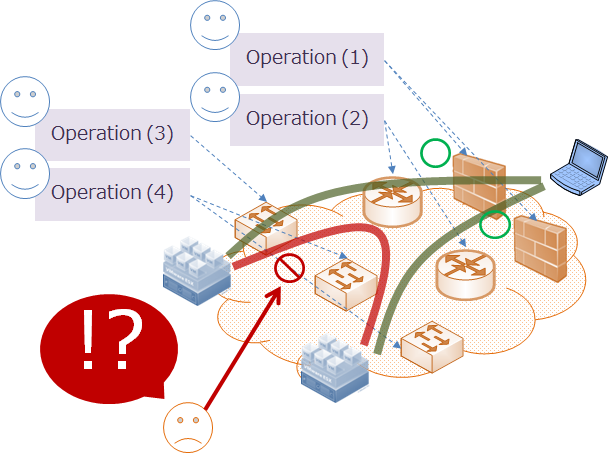
\includegraphics[scale=0.6]{img/difficulty-of-network-operation.png}
  \caption{ネットワーク全体の動作確認の難しさ}
  \label{fig:difficulty-of-network-operation}
 \end{figure}

ネットワーク全体としての動作保証の難しさは以下のような要素に起因すると考
えられる。
\begin{itemize}
 \item ネットワークでは機器それぞれが様々なポリシをもとにトラフィックを
       制御する。それらは周囲の機器と交換される制御情報、実際にながれて
       いるその時々のトラフィックなどにも影響される。
 \item ネットワーク全体の動作は隣接する機器間で相互に設定情報の整合性を
       とる必要があり、使用している機器や技術の数が増加するほど検討すべ
       き組み合わせのパターンが増大する。
\end{itemize}
こうした理由から、大規模なネットワークや、仮想化技術などをつかった複雑性・
共有度が高くかつ動的な構成変更がおこなわれるネットワークでは、ネットワー
クに対する設定変更・構成変更の影響範囲を正確に判断することは非常に難しく
なっている。

  \section{従来のネットワークテストとネットワークテストに着目する理由}

  % 運用の理想像や現状
  % TODO: ITHD技術交流会資料
  % \url{https://drive.google.com/drive/folders/0B2eRR_JxYJA5OFkzUFlveVlObWc}
  % p6-7 あたりとかの話をいれる

ここまで、\ref{sec:system-problem}節にあげたように、ネットワークの構築や
運用でどのような課題があるかをみてきた。こうした課題があることにより、従
来のネットワーク(特に高いサービスレベルが要求されるシステムのネットワー
ク)の構築・運用では以下のような状況がみられる。
\begin{itemize}
 \item ネットワークの構成変更などをおこなう際は、その物理構成操作の要求
       やトラブル発生時の現地対応リスクなどを加味して、特定の場所に人や
       端末を配置しながら人手でテストを実行していくという、人海戦術的オ
       ペレーションをとる。
 \item 特定の設定変更によってどの程度のサービス影響があるのか判断するこ
       とが難しいため、機器ごとやサービスごとなどの知見者をあつめて、変
       更した場合の影響検討をくりかえしおこなう。(複数回のレビューをおこ
       なう。)
\end{itemize}
いずれにせよ、これらは現地・現物・人海戦術的なやりかたとなる傾向があり、
システム(サービス)にもとめられる迅速性(agility)を落とすボトルネックにな
りがちである。

影響範囲予測の難しさへの対策として、検証環境を用意して、そこで実際に想定
されるオペレーションを実行することもおこなわれる。しかし、ネットワーク規
模や構成の大規模化・複雑化とそれによるテストパターン数の増大にともない、
テストパターンをすべて人手で網羅することは非常に難しい。そのため以下のよ
うな状況(リスク)を受け入れざるをえない状況がある。
\begin{description}
 \item[テスト作業用リソースの確保] 通常、テストをおこなうための人・機器
            の準備には制約がある。人手による作業の場合、作業コスト・時間
            や規模がどうしてもスケールさせられないため、小規模なオペレー
            ションで は十分なテストができないまま本番環境での作業になる
            傾向がある。
 \item[本番環境と検証環境の差分] リソース確保の都合、多くの場合では検証
            環境と本番環境では使用する機材や構成などに違いがある
            \footnote{同一製品ラインだがスペック・ライセンスのことなるも
            のをつかう、あるいは仮想アプライアンス版で検証をおこなう、な
            どが検証環境での選択肢としてあるが、特定の機器や機能の組み合
            わせ、特定のハードウェアやソフトウェアでのみ発生するトラブル
            などもある。}。また、実際にネットワーク内部を流れるトラフィッ
            クなどを再現するのは非常に難しい\footnote{特に非機能要件、性
            能や可用性要件などを検証環境で保証することはむずかしい。環境
            を段階的に拡張した結果として性能問題がおきる、特定の利用者に
            よる過負荷によりトラブルがおきるなど、事前・別環境での再現が
            難しい問題がある。}。そのため、検証環境では発生しなかった問
            題やトラブル、影響の見落としが本番環境の作業ではじめてあらわ
            れることがある。
 \item[代表パターンのみのテスト] 縮小したテストケースではどうしても一部
            の設定ミスや不整合などを見落とすリスクがある。
 \item[テスト結果判断のばらつき] 手順書の解釈、操作の実行や結果の取得・
            判断などがテスト実行者に依存するため、本来問題となる事象を見
            落としてしまうリスクがある。
\end{description}

%%% Local Variables:
%%% mode: yatex
%%% TeX-master: "main.tex"
%%% End:

%% -*- coding: utf-8-unix -*-

\chapter{課題に対するアプローチ}
\label{chap:approach}

% なぜ「テスト」が必要なのか? という話をいれるか?

大規模化・複雑化するネットワークでは、検証環境での手作業によるテストや人
による多重レビューによってサービス影響や問題点を完全に洗い出すのは、時間
的・リソース上の制約によって非常に困難である(\ref{chap:problem-setting}
章)。こうした課題に対して、本プロジェクトは以下のようなアプローチで対応
を試みる。
\begin{description}
 \item[テストを自動化する] 自動化することにより、人力ではできない速度で、
            人力では見きれない範囲(パターン)をテストする。
 \item[実機・実際のシステムをもとにテストをする] 本番環境をどこまで検証
            環境で再現するかというリソース問題は残るが、テスト対象ネット
            ワークとしては特定のソフトウェア/ハードウェアを区別しない。
            一般的かつ実際に使用しているネットワークを自動テスト可能にす
            る。
\end{description}


\section{自動テストの基礎知識}
\label{sec:latedge-test-automation}

 % NetTester機能拡張検討
 % \url{https://drive.google.com/file/d/0B2eRR_JxYJA5TmhaeWItNF93Um8/}
 % ITHD技術交流会資料
 % \url{https://drive.google.com/drive/folders/0B2eRR_JxYJA5OFkzUFlveVlObWc}
 % ool意見交換会1019
 % \url{https://drive.google.com/drive/folders/0B2eRR_JxYJA5NHcxX0ZuTm9ZTEk}

  \subsection{自動テストの一般的な動向}
  \label{sec:popular-test-automation}

ソフトウェア開発においては、システム(アプリケーション)の自動ビルド・自動
デプロイ・自動テストなどがおこなわれ、特に近年では CI/CD や DevOps といっ
た形でノウハウやベストプラクティスの蓄積・共有、ツールや環境の整備といっ
た取り組みをすることが一般的になった。

また、クラウドサービスへのシフトを背景に、アプリケーション(ソフトウェア)
だけでなくシステム基盤についても、ソフトウェアによる構築や制御が可能になっ
てきた。ソフトウェアによってシステム基盤全体を制御するという考え方は、
IaC (Infrastrucure as Code) や SDx(Software Defined Anything) /
SDI(Infrastructure) / SDDC(DataCenter) など様々なコンセプトで実現される
ようになってきている。

CI/CDやDevOpsなどの取り組みは、単なるソフトウェア開発の範囲だけでなく、
ソフトウェアによって制御可能な(クラウドサービスベースの)システム基盤を含
むシステム(あるいはサービス)全体で取り組まれるようになっている。こうした
取り組みでは、アプリケーションとシステム基盤全体の構築・運用を最適化し、
システムの利用者への価値提供 = サービス価値を最大化することをねらってい
る。

  \subsection{「ふるまい」のテスト}
  \label{sec:behavior-test}

  % サービスのテストとは? →二重の円の図
  % なぜトップダウンにやるべきなのか
  % (無駄なテストをさける/DHHのはなし:高宮さんTremaday沖縄資料, TDD/BDDまわりの話)
  % \url{https://3.basecamp.com/3088280/buckets/867009/uploads/317155391}

\ref{sec:popular-test-automation}節で取り上げたように、CI/CDといった開発・
運用プロセスのとりくみがソフトウェア開発分野を中心におこなわれている。本
プロジェクトではそうした考えかたをシステム基盤(ネットワーク)の構築・運用
に適用していくことを考える。ネットワークのテストを自動化するにあたって、
ソフトウェアの自動テストなどで確立されたベストプラクティスやツールなどを
応用するかたちになることが効果的だと言える。そこで、本プロジェクトでは、
ネットワークをBDD(Behavior Driven Development)の考えかたをもとにテストす
ることを考えた。

BDDはTDDから派生した開発手法で、開発するソフトウェアに期待される「ふるま
い」に対するテストである~\cite{wikipedia-bdd}。BDDではソフトウェアに期待
される「ふるまい(Behavior)」、つまり、ソフトウェアの複数の機能を連結した
end-to-end でのインテグレーションテストを行なう
(\figref{fig:test-difference})。

\begin{figure}[h]
 \centering
 \begin{minipage}[c]{0.45\columnwidth}
  \centering
  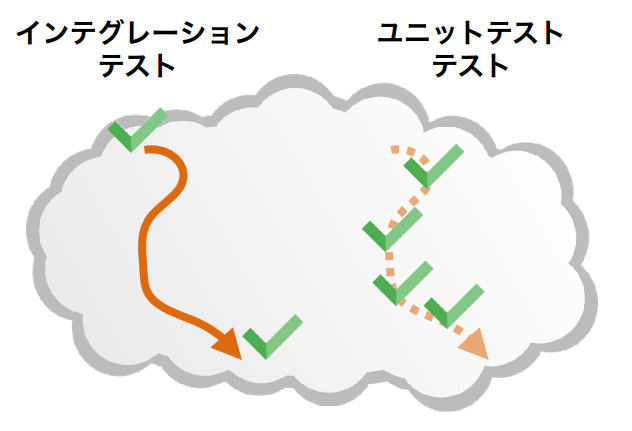
\includegraphics[width=\columnwidth]{img/test-difference.png}
  \caption{インテグレーションテストとユニットテスト}
  \label{fig:test-difference}
 \end{minipage}
 \begin{minipage}[c]{0.45\columnwidth}
  \centering
  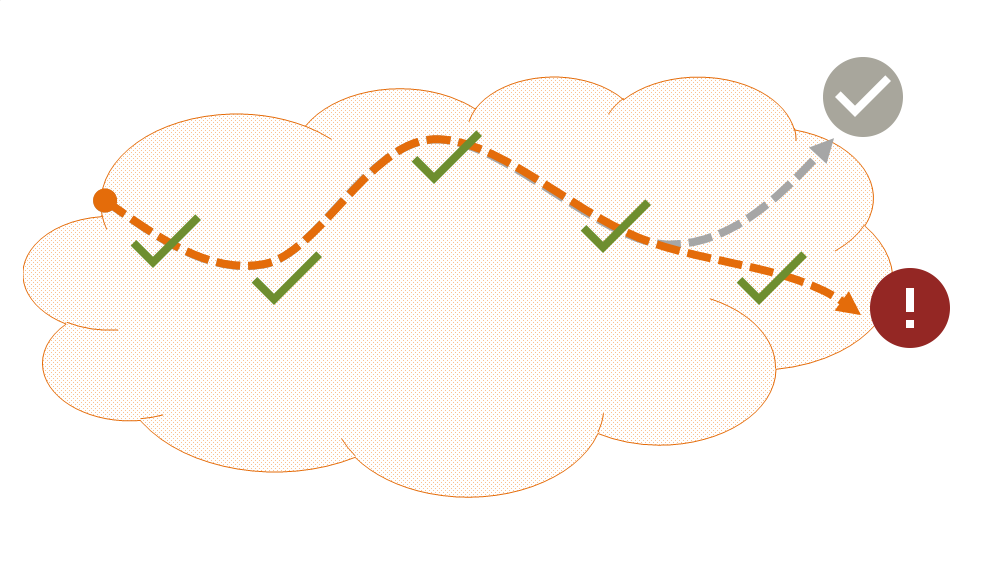
\includegraphics[width=\columnwidth]{img/test-difference2.png}
  \caption{ユニットテストの課題}
  \label{fig:test-difference2}
 \end{minipage}
\end{figure}

\begin{wrapfigure}{r}{16zw}
 \vspace*{-\intextsep}
 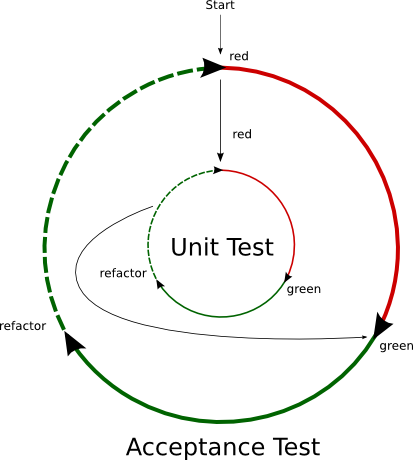
\includegraphics[width=16zw]{img/bdd-cycle.png}
 \caption{BDDサイクル\cite{bdd-cycle-figref}}
 \label{fig:bdd-cycle}
\end{wrapfigure}

仕様(spec)にもとづいたインテグレーションテストを最初におこなうようにする
ことで、以下のようなメリットがある。
\begin{itemize}
 \item テストの目的を明確にする
 \item 実際的なテストができる
 \item 無駄なテストをおこなわない
\end{itemize}

BDDでは、まずインテグレーションテスト(仕様上期待されるふるまい)について
のテストをおこない、問題があった場合に内部を詳細化したユニットテストに分
割して原因をきりわけるようにする(\figref{fig:bdd-cycle})。

インテグレーションテストがパスすれば詳細なテストを省略し、インテグレーショ
ンテストで失敗した場合にユニットテストを実施して原因の切り分け・修正をお
こなう。こうすることによって、不要なユニットテストの実装・実行にともなう
開発効率の低下を回避し、最終的にシステム(ソフトウェア)の利用者に対して価
値を提供しているか(期待される仕様を満たすか)どうかを基準にテストをおこな
う。インテグレーションテストでは、テスト対象とするシステム(ソフトウェア)
の最終的なふるまいをテストするため、仕様とテストシナリオがほぼ直接マッチ
する。したがって、BDDのテストシナリオを記述する作業は製品が満たすべき仕
様を具体的に定義したものとなる。

通常、テストコードは直接的に金銭的報酬を発生させるものではなく、開発にお
いてテストによる品質担保とテスト対象(プロダクト)とのバランスを適切に保つ
必要がある。ユニットテストなどの詳細化された機能単位のテストでは、個々の
機能としての動作は確認できるが、複数の機能を組合せ・連結して最終的にどの
ような動作をするか、というテストとの対応が結びつけにくい
(\figref{fig:test-difference2})。

こうした状況では、往々にして「ユニットテストをもれなく作成すること」「テ
ストカバレッジを100\%にすること」が目的化されがちである。しかしもちろん、
個々のユニットテストがパスしても、最終的にテスト対象となる製品が(利用者
が求める)仕様を満たさなければ価値がない。BDDでは最終的に製品が満たすべき
仕様に着目し、テスト対象が実現すべき価値の観点で無駄なテストを減らすこと
を想定している。

 \section{理想像とプロジェクトのターゲット}
 \label{sec:desired-and-target}

 % 理想的にはどうなってほしいのか
 % ここではどこらへんをおとしどころにするか

  \subsection{テストしたいネットワークの「ふるまい」}
  \label{sec:behavior-to-test}
  % ネットワークの「ふるまい」とは何か?
  % 動的なテスト, 静的なテストとは何か?

\ref{sec:behavior-test}に示したとおり、本プロジェクトではBDDの考えかたに
そって、ネットワークの「ふるまい」をテストする。ネットワークのふるまいと
して、大きく下記の2点を考える。
\begin{itemize}
 \item 静的なふるまい
 \item 動的なふるまい
\end{itemize}

    \paragraph{静的なふるまい}
ネットワークが定常状態にあるときに、end-to-end でどのような通信ができる
か(end-to-endの通信試験: \figref{fig:test-static})。ネットワークにもとめ
られ最も基本的なる機能要求は、必要なノード間/アプリケーション間で通信が
できることである。静的なふるまいとして、ネットワークの状態がかわらない
(一定のトポロジ/一定の状態、例えば、通常利用していて特にイベントが発生し
ていない状況)ときに、アプリケーションレベルでの通信が実現できる(できない)こ
とを確認する。
% 図をいれる: net_tester/examples readme にいれたやつ。
\begin{figure}[h]
 \centering
 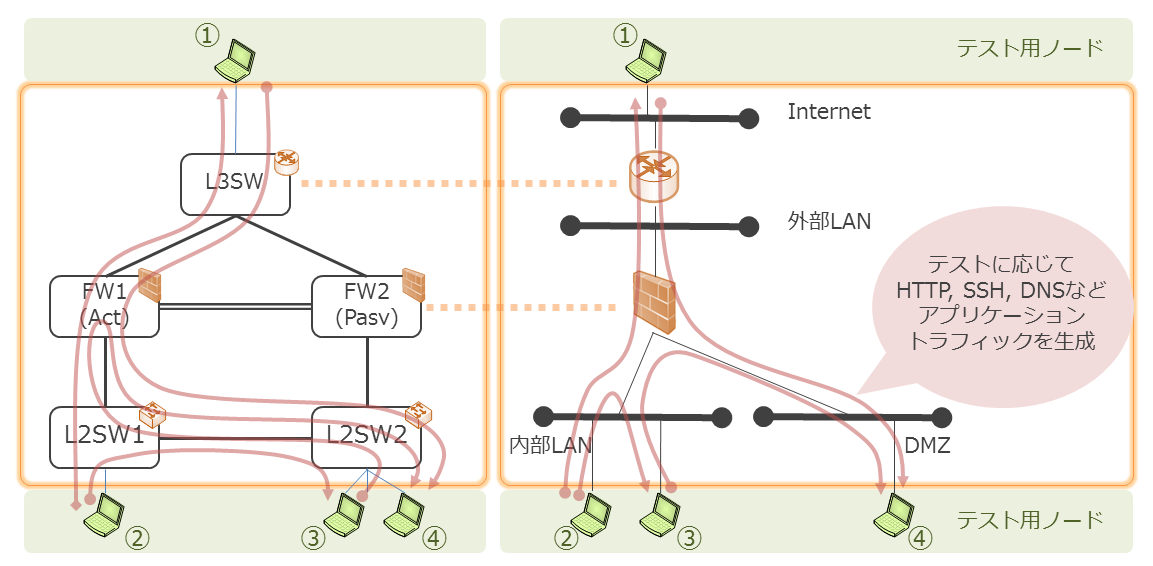
\includegraphics[scale=0.5]{img/test-static.png}
 \caption{ネットワークの静的なふるまいのテスト}
 \label{fig:test-static}
\end{figure}

このような通信試験においては、適切な場所(物理的・論理的な位置)にノードを
設置すること、なるべく実際的な(実際利用されたときに発生するトラフィック
に近い)テストトラフィックを発生させることがポイントとなる。

    \paragraph{動的なふるまい}
ネットワークは、耐障害性・拡張性を保証するために、ネットワーク機器間で相
互に制御情報を交換し、動的にネットワーク全体のトラフィック制御をおこなう。
\footnote{たとえば、ある機器に障害が発生し、その機器でトラフィックが中継
できないと(周囲の機器が)判断した場合、その機器を中継しないようにネットワー
クのトラフィック転送ルールが再構成される。}こうしたネットワーク自身の状
態変化がともなう状況を動的なふるまい、ととらえる。

定常状態にあったネットワークで、イベントに対して動的なふるまいが発生する
と、ネットワークの状態\footnote{トポロジ、あるいはNW機器の持つ状態(経路
情報, Acitve/Standbyなどの状態など)}が別の定常状態へと変化する。状態変化
の過程では、利用しているネットワーク機器の機能や仕様により、テストトラ
フィックパスが変更され、一時的に転送が中断/再開したりする。動的なふるま
いのテストは、こうした状態遷移中の通信状況を確認するものである
(\figref{fig:test-dynamic})。
% 図をいれる: net_tester/examples readme にいれたやつ。
\begin{figure}[h]
 \centering
 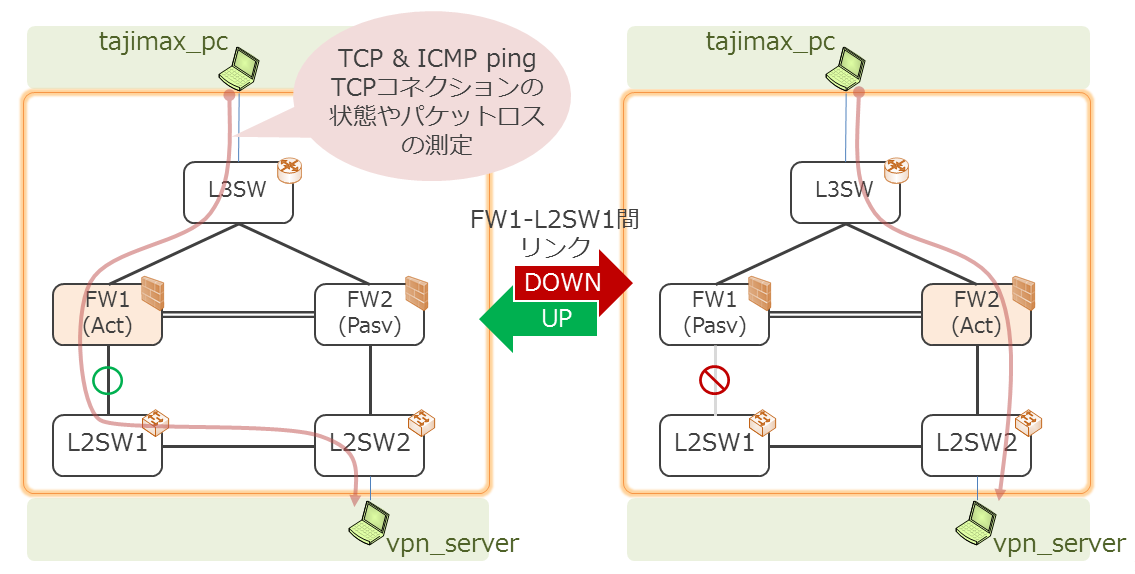
\includegraphics[scale=0.5]{img/test-dynamic.png}
 \caption{ネットワークの動的なふるまいのテスト}
 \label{fig:test-dynamic}
\end{figure}

動的なふるまいのテストでは、テスト対象ネットワークでの状態変化イベントの
発生、イベントをまたいだテストトラフィックの生成や通信状況の判断がポイン
トとなる。

  \subsection{ネットワークの自動テストと運用プロセス}
  \label{sec:network-test-and-process}

  % 既存の(ソフトウェア開発の)ツールや方法論が応用できること
  % だれに対して、どのようなメリットを提供するか?

\ref{chap:problem-setting}章で解説したように、現状ネットワークのテストは
人手によるところが多く、それがボトルネックになって網羅性やスケール性が低
い。ここでは、もし仮に、現状人手に頼らざるをえないネットワークの操作が機
械的に・自動実行できるとしたらどのような構築・運用プロセスをとることがで
きるかについて検討する。

ソフトウェアによってネットワークの操作が自由にできる(操作の自動化ができ
る)と仮定した場合、ネットワークに対する構築や運用についても、ソフトウェ
ア開発でおこなわれているベストプラクティスやノウハウがそのまま応用できる
形となることが理想的だと考える。これによって、
\figref{fig:desired-cicd-process}のようなかたちでシステムの自動構成・自
動テスト、本番システムデプロイというCI/CDプロセスを実現させることができ
る。
\begin{itemize}
 \item システム(ネットワーク)で実現すべき要求を定義する
 \item 要求をコード化する
       \begin{itemize}
        \item 要求を実現するためのコード(ネットワーク設計/実装)
        \item 要求を確認するためのコード(ネットワークが満たすべき「ふる
              まい」: ネットワーク上で実現されるべき通信やネットワーク自
              身の動作)
       \end{itemize}
 \item 検証環境で自動構築・自動テストをおこなう
       \begin{itemize}
        \item テストが失敗したら原因を分析し、コードを修正・再テストをおこなう
       \end{itemize}
 \item 自動テストがすべてパスしたら本番環境へのデプロイをおこなう
\end{itemize}

% 図をいれる: ぐるぐるまわす図
\begin{figure}[h]
 \centering
 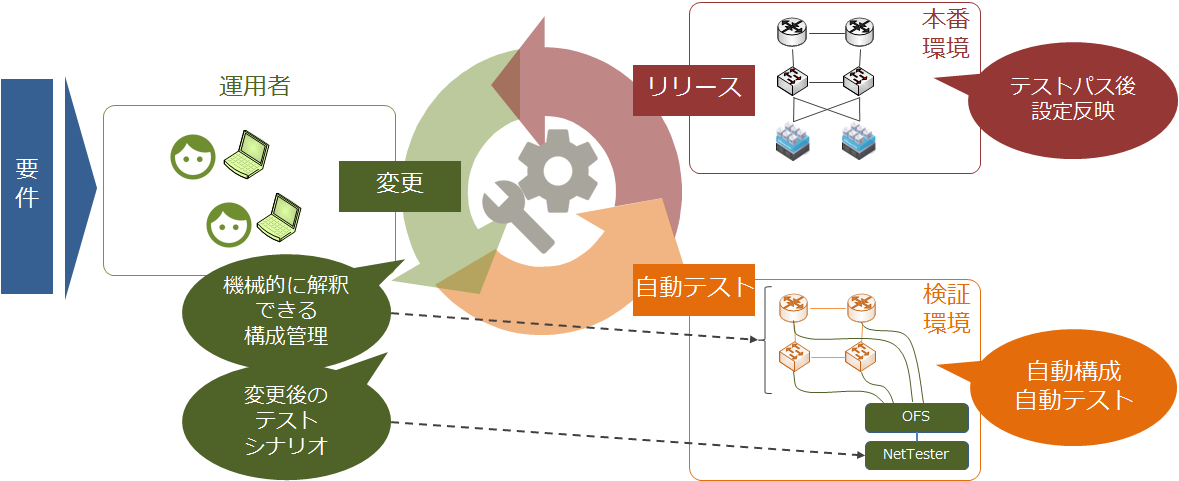
\includegraphics[scale=0.5]{img/desired-cicd-process.png}
 \caption{ネットワークのCI/CDプロセス}
 \label{fig:desired-cicd-process}
\end{figure}

ネットワーク(に限らずシステム基盤)では、ハードウェア製品を多様するため本
番環境とまったく同等の検証環境を整備することは通常難しい。しかし、性能面・
拡張性の問題などをある程度スコープ外とすることで、仮想アプライアンスなど
を利用して小規模でも機能的には同等の環境を整備することができるようになっ
ている。このように、仮想化技術の応用をふくめて、機器/環境をソフトウェア
で制御できる範囲がひろがり、自動化されるにともない、まず自動構築のための
技術・ツール・ノウハウが発展しつつある。

本プロジェクトは、そこに(ネットワークの)テストという構成要素を補い、上記
のようなシステム基盤のCI/CD実現を促進させることを狙っている。

 \section{ネットワークテストシステムの検討}
 \label{sec:discuss-network-test}

 % OOD発表資料p.4-5 「6個の構成要素」の話。ここでターゲットにするものは何か?
 % ネットワークの操作を自動化するために必要なことは?
 % テストの自動化のためにどういった機能コンポーネントが必要か?

ネットワークのテストを自動化するにあたって、現状手作業でおこなっている操
作を機械的に実行できるようにしなければならない。本プロジェクトでは、ネッ
トワークのテストのために必要な操作を
\figref{fig:features-of-network-testing}・\tabref{tab:test-functions}の
ように分類している。

\begin{figure}[h]
 \centering
 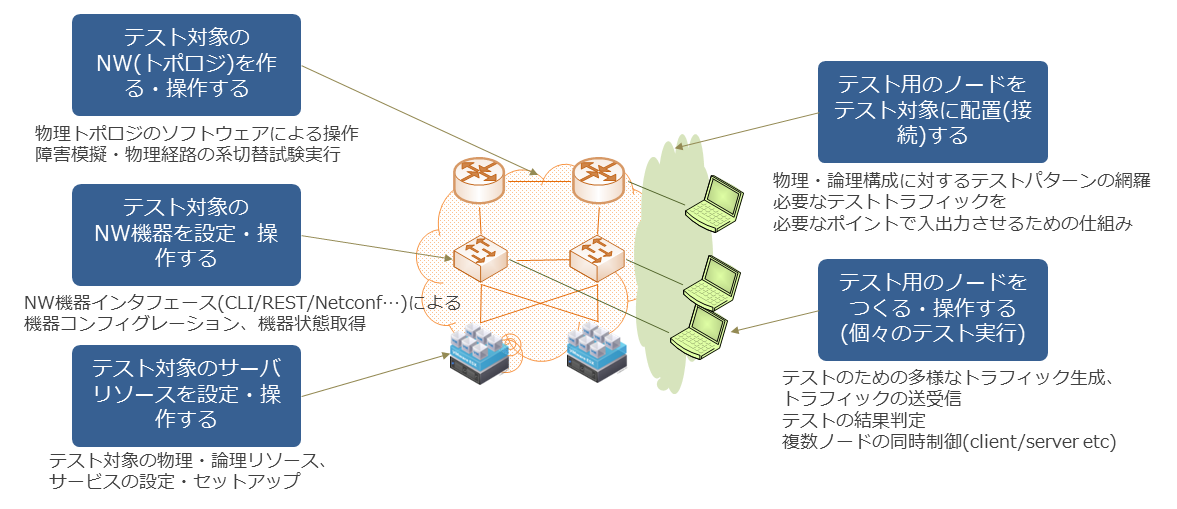
\includegraphics[scale=0.5]{img/features-of-network-testing.png}
 \caption{ネットワークテスト自動化のための機能要素}
 \label{fig:features-of-network-testing}
\end{figure}

\begin{table}[h]
 \caption{NWテスト自動化に必要な機能要素}
 \label{tab:test-functions}
 \begin{tabularx}{\linewidth}{l|l|X}
  \hline
  No. & 要素 & 役割 \\ \hline
  \hline
  1 & NW機器を設定・操作する & テスト対象ネットワークにあるNW機器の設定を変更する \\ \hline
  2 & サーバリソースを設定・操作する & テスト対象ネットワークにある物理サーバ・仮想サーバのリソース操作などをおこなう \\ \hline
  3 & トポロジを操作する & テスト対象ネットワークのトポロジをソフトウェアによって操作する \\ \hline
  4 & テスト用ノードを配置する & テスト用のノードを生成し、テスト対象ネットワークの指定した箇所に配置(接続)する \\ \hline
  5 &テスト用ノードを操作する & テスト用のノードを操作し、テストトラフィックの生成をおこなう\\ \hline
 \end{tabularx}
\end{table}

    \paragraph{テスト対象NW内ノード操作}
\tabref{tab:test-functions} No.1-2 はテスト対象ネットワークを構成する機
器(ハイパーバイザなど仮想化基盤管理・操作を含む)である。こうした機器操作
のための技術・ツールなどは既に多数存在しているため、本プロジェクトではこ
こには注力しない。(既存の技術やツールを応用する;
\ref{sec:related-research}節参照。)

    \paragraph{トポロジ操作}
\tabref{tab:test-functions} No.3 はテスト対象ネットワークのトポロジ(物理
結線を含む)の操作である。障害試験(リンクダウンなど)や環境の構成拡張・縮
小(ノードの追加・削除などトポロジ変更)といった、ネットワークトポロジその
ものの変更が発生する際のネットワークのふるまいをテストするために必要とな
る。

\ref{sec:difficulty} で示したように、特に物理構成要素の操作は自動化がむ
ずかしい。\lopjc では、OpenFlow スイッチを応用したテスト対象ネットワーク
の物理トポロジ構成・操作についての実証実験を行なった。本プロジェクトでは
そこで実証した技術を応用してテスト対象ネットワークの物理トポロジ操作をお
こなう。

    \paragraph{テスト用ノード操作}
\tabref{tab:test-functions} No.4-5 はテスト用ノードの操作である。一般的
に、ネットワークのテストではテスト用のトラフィックの生成・受信をおこなう
ことによって、テスト対象ネットワークが問題なく動作しているかどうかを確認
する。テストトラフィックの送受信はテスト対象ネットワークを構成する機器
(NW機器やサーバ)を利用場合もあるが、ログ取得やテスト用ツール準備などの都
合から、何らかのテスト用ノード(PCなど)を別途用意することが多い
\footnote{特に新規構築の場合は、サーバ等テスト対象とするノードが利用でき
ない(存在しない)状態でネットワークのテストをおこなうこともある。}。こう
したテスト用ノードを利用したテストには以下のような問題がある。
\begin{itemize}
 \item テスト用ノード(機器台数)の上限
 \item テスト用ノードを操作する人(担当者人数)の上限
 \item 分散作業によるテスト全体での状況把握の難しさ
 \item テスト用ノードのセットアップ(IPなど)の手間
 \item テスト用ノードの配置(テスト対象NWへの接続)の手間
\end{itemize}

トポロジ操作同様に、\lopjc では、Linux Namespace を利用したテスト用ノー
ドの生成・集中制御とOpenFlow スイッチを応用したテスト用ノード配置につい
ての実証実験を行なった。本プロジェクトではそこで実証した技術を応用して、
より実用的なテストユースケース(テストシナリオ)の実現をおこなう。

 \section{基本的なアイディア}
 \label{sec:basic-tester-idea}

  % このプロジェクトでは、
  % 「ネットワークテストシステム」としてどういったシステムを作ろうとしたのか?
  % NetTester の基本的なアイディアというか、
  % そもそものパッチパネルベースにテストをやるっていう話

  % https://drive.google.com/file/d/0B2eRR_JxYJA5TmhaeWItNF93Um8/view
  % にある「もうちょっと一般化」くらいの粒度でいれてもいいかもしれない。

\ref{sec:discuss-network-test}節でネットワークのテスト自動化のために必要
な機能要素について解説したが、それらをもとにネットワーク「テスタ」に求め
られる機能要求について解説する。要求については \lopjtech も参照のこと。

ネットワークのテスト自動化では、従来手作業でおこなっていたのと同等の操作
を、ソフトウェアにより自動的かつプログラマブルに実現したい。そのために、
テスト対象ネットワークの物理トポロジを、テストシナリオに応じて動的に再構
成したり、テスト用のノードを動的に接続したりする
(\figref{fig:basic-idea})。そこで、様々なノード間をつなぎ合わせる機能を
準備する(\tabref{tab:test-functions} No.3-4)。

% patch model の基本的な概念図をいれる
% net-tester readme にある最初の図くらいのやつでよい。
\begin{figure}[h]
 \centering
 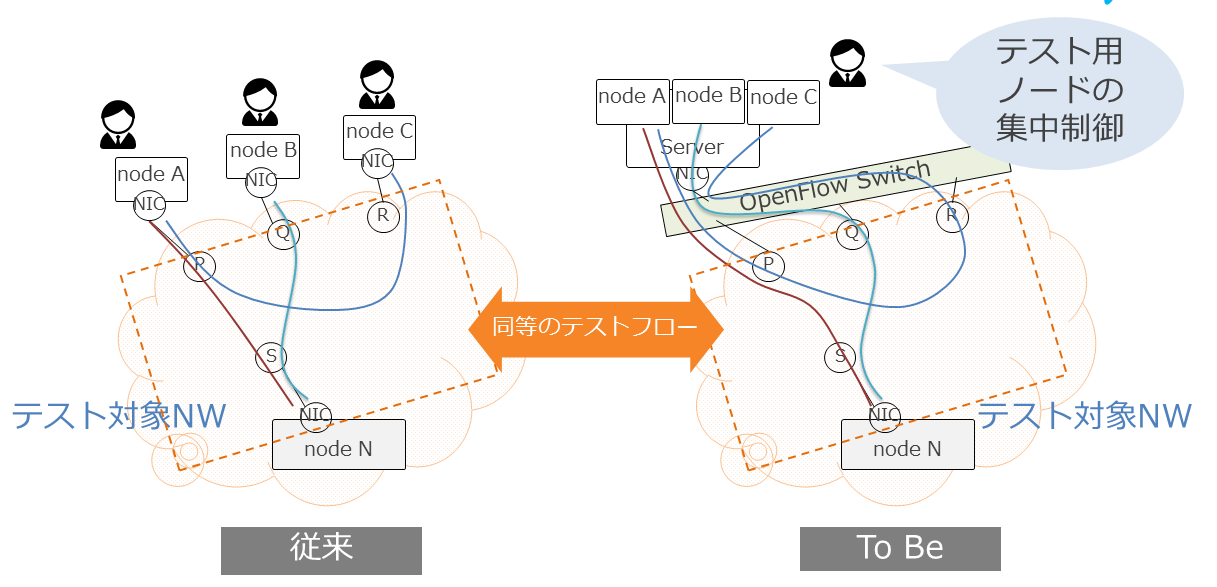
\includegraphics[scale=0.5]{img/basic-idea.png}
 \caption{テスターの基本アイディア}
 \label{fig:basic-idea}
\end{figure}

\lopjc では、安価かつトラフィック制御を自分で操作(プログラミング)可能な
OpenFlowスイッチを利用して、物理配線操作をするパッチパネルと同等のものを
実現し(\figref{fig:poc-l1patchpj}: \tabref{tab:test-functions}参照)、簡
単なテストユースケースのもとで有効性を確認した。

\begin{figure}[h]
 \centering
 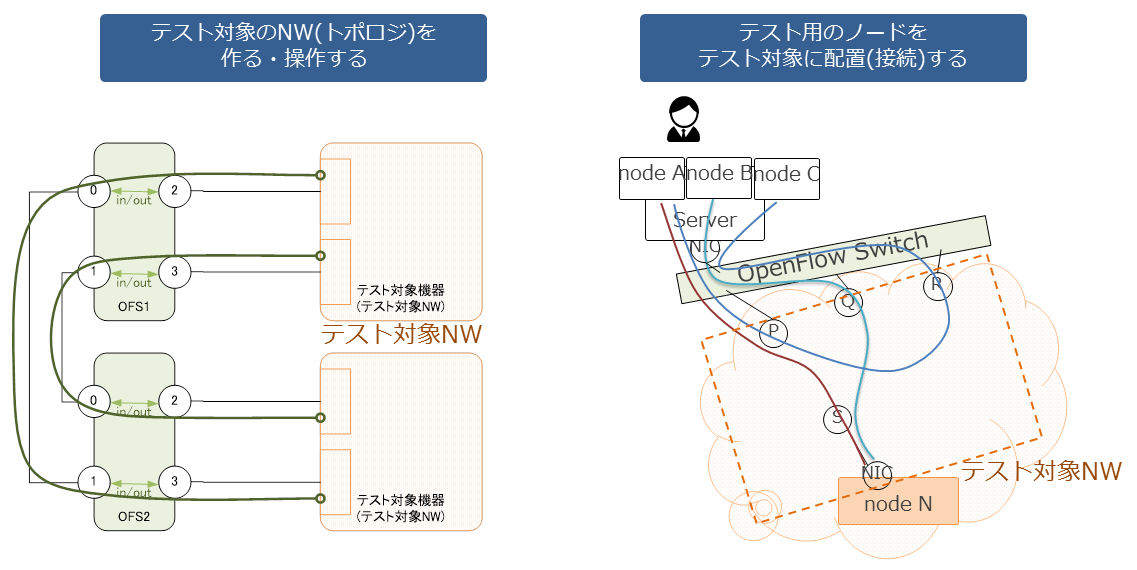
\includegraphics[scale=0.5]{img/poc-l1patchpj.png}
 \caption{\lopj PoCで実装・実証した機能要素}
 \label{fig:poc-l1patchpj}
\end{figure}


   % 「テスタ」に求められることは何か?
   % "patch panel" model – NetTester
   % \url{https://3.basecamp.com/3088280/buckets/867009/documents/208275139}
   % いるか??

 本プロジェクトは、\lopj の結果をもとに、NetTester~\cite{nettester} とい
 うテストツールを開発した。NetTester について
 は~\ref{chap:nettester-design}章・\ref{chap:nettester-usage}で解説する。
 また、NetTesterをつかったネットワークテストのユースケース実証について
 は~\ref{chap:poc-target-design}章・\ref{chap:poc-scenario-dev}で解説する。


%%% Local Variables:
%%% mode: yatex
%%% TeX-master: "main.tex"
%%% End:

%% -*- coding: utf-8-unix -*-

\chapter{NetTesterの技術仕様}

\section{モデル}

NetTester の構成(モデル)

つかっている技術:
\begin{itemize}
 \item network namespaceとその操作, trema/phut
       \begin{itemize}
        \item Phut Memo – NetTester \url{https://3.basecamp.com/3088280/buckets/867009/documents/238439817}
       \end{itemize}
 \item patch panel 実装, ActiveFlow
       \begin{itemize}
        \item パッチの概要 → パッチ – NetTester \url{https://3.basecamp.com/3088280/buckets/867009/documents/213266851}
        \item "patch panel" model – NetTester \url{https://3.basecamp.com/3088280/buckets/867009/documents/208275139}
       \end{itemize}
\end{itemize}

phut, activeflowなどの実装寄りのはなしは付録とかにするか。

\section{フロールール設計}

2015年度実装に対してあるていど簡略化した実装になっているのでそのへんのはなし。

flowの優先度
\begin{itemize}
 \item テスト対象NW→Host(テストノード)へのbroadcastのコントロール – NetTester \url{https://3.basecamp.com/3088280/buckets/867009/todos/198950295}
 \item NetTester機能拡張検討
       \url{https://drive.google.com/file/d/0B2eRR_JxYJA5TmhaeWItNF93Um8/view}
       いくつのフロー案とどれを、なぜ選択したのか、という話
 \item Table \& Rule Priority Design (2015 ool-l1patch) – NetTester \url{https://3.basecamp.com/3088280/buckets/867009/documents/211290387}
 \item Table \& Rule Priority Design (NetTester) – NetTester \url{https://3.basecamp.com/3088280/buckets/867009/documents/217426690}
       \begin{itemize}
        \item default deny の要否: packet-in をいれるかどうか → デバッグ用途のはなし?
        \item packet-in による trema の trouble/trouble shoot → 補足とかでいれる?
              \begin{itemize}
               \item 謎PacketInで死なずにログを出す – NetTester \url{https://3.basecamp.com/3088280/buckets/867009/todos/221324759}
               \item 調査: テスト環境でOFS(Pica8)-OFC(NetTester/Trema)の接続が切れる – NetTester \url{https://3.basecamp.com/3088280/buckets/867009/todos/218484578}
              \end{itemize}
       \end{itemize}
 \item VLAN Trunk Portを使ったテストシナリオを作る – NetTester \url{https://3.basecamp.com/3088280/buckets/867009/todos/238166429}
 \item テスト対象NW機器間接続patch機能を作る – NetTester \url{https://3.basecamp.com/3088280/buckets/867009/todos/238169839}
\end{itemize}

\section{リンク操作方式}

\begin{itemize}
 \item テスト対象NW機器間接続のup/down方式を決める – NetTester \url{https://3.basecamp.com/3088280/buckets/867009/todos/238171702}
 \item リンクダウン・リンクアップ機能用のスクリプト実装 – NetTester \url{https://3.basecamp.com/3088280/buckets/867009/todos/247379766}
\end{itemize}

\section{制限・制約}

モデルから: 拡張性に関するはなし

フロールールから: arp があるていどみえてしまうこと → セキュリティについて?

DPIDや一部のポート番号の固定について
\begin{itemize}
 \item NetTesterの実装で気になるところ – NetTester \url{https://3.basecamp.com/3088280/buckets/867009/todos/196940380}
\end{itemize}

NetTester 自体の通信要件?
\begin{itemize}
 \item openflow, ssh, syslog 等
\end{itemize}


%%% Local Variables:
%%% mode: yatex
%%% TeX-master: main.tex
%%% End:

%% -*- coding: utf-8-unix -*-

\chapter{NetTesterの使いかた}
\label{chap:nettester-usage}

NetTesterによるテスト環境の構築方法やシステム要求、本PoCでの実際に使用し
た構成や機器・ソフトウェアの情報、基本的な使用方法について解説する。

 \section{NetTesterのデプロイ}
 \label{sec:nettester-deployment}

  \subsection{物理OpenFlowスイッチ}
  \label{sec:nettester-deploy-psw}

  % 物理OFSのデプロイ
  % - pica8 (OVS) の設定について
  %   - Portの設定(VLAN) : [L1PJTECH] 参照
  %   - \code{fail\_mode} の設定
  %     \url{https://docs.google.com/document/d/1yBn8S3DOhkuaVuVtUmwOeyvQxWm1v6_PfWTj3iDcx0U/}
  %   - inactivity probe の設定:
  %     調査: テスト環境でOFS(Pica8)-OFC(NetTester/Trema)の接続が切れる – NetTester
  %     \url{https://3.basecamp.com/3088280/buckets/867009/todos/218484578}
  %     \url{https://docs.google.com/document/d/1_-pLOXSOLutRb1_-tlcb_FwLCHq3Y7zQxp79_qXjDiM/}
  %     (そんなに重要じゃないけど一応)
  %   - 毎回ofsがcontrollerに繋いでくるのを待つ(10秒)のをどうにかしたい – NetTester
  %     https://3.basecamp.com/3088280/buckets/867009/todos/211396447

\ref{sec:nettester-model}節に示したとおり、NetTester は1台の物理OpenFlow
スイッチを利用して、テスト対象ネットワークへの接続をおこなう(物理
OpenFlowスイッチを使用してテストトラフィックを''distribute''する)。本節
では物理OpenFlowスイッチの選択と設定について解説する。

    \paragraph{物理OpenFlowスイッチの要件と選択}
NetTesterが使用する物理OpenFlowスイッチには\tabref{tab:ofs-requirement}
の要件~\cite{l1pjpoc}が求められる。

\begin{table}[h]
 \centering
 \caption{OpenFlowスイッチ要件(OpenFlow/1.0)}
 \label{tab:ofs-requirement}
 \begin{tabular}{l|l}
  \hline
  分類 & 項目 \\
  \hline
  \hline
  Match  & In-Port \\ \cline{2-2}
         & VLAN ID \\ \cline{2-2}
         & Source/Destination MAC Address \\ \hline
  Action & Out-Port \\ \cline{2-2}
         & Push/Pop VLAN ID \\ \hline
  Other & Priority \\
  \hline
 \end{tabular}
\end{table}

本プロジェクトでは昨年度実施した \lopj の環境を継続しており、
\tabref{tab:psw-list}に示すOpenFlowスイッチを使用している~\cite{l1pjpoc}。
(2台のOpenFlowスイッチを使用して Tester
set\footnote{\ref{sec:mgmt-and-tester-nw}節参照。} を2セット構築している。)
% TODO: Tester set の説明

\begin{table}[h]
 \centering
 \caption{物理OpenFlowスイッチ}
 \label{tab:psw-list}
  \begin{tabular}{l|l|l}
   \hline
   Host name & Hardware & OS/Version \\
   \hline
   \hline
   OFS1 & Quanta T1048-LB9 & PicOS 2.5.2 / Revision 19975 \\
   OFS2 & Pica8 P-3290 & PicOS 2.2.1S3 / Revision 14775 \\
   \hline
 \end{tabular}
\end{table}
% TODO: 昨年度ドキュメントそのまま。現物確認すること
% TODO: OVS version を追記すること。

    \paragraph{物理OpenFlowスイッチの設定}
PicOSはOVS Mode (Open vSwitch)で使用する。物理スイッチ(PicOS OVS)では以
下の設定をおこなう。下記設定事項についてはPicOSマニュアルおよびOpen
vSwitchドキュメント~\cite{ovs-vswitchd-doc}も参照すること。
\begin{itemize}
 \item パッチとして使用するすべてのポートの設定~\cite{l1pjtech}
       \begin{itemize}
        \item VLANの操作をおこなうため、VLAN Mode を trunk として設定
              (\verb|vlan_mode=trunk|)する:
        \item テスト対象ネットワークで発生するブロードキャスト転送の抑制・
              STPへの干渉をさけるため、フラッディングの無効化
              (\verb|no-flood|)およびSTPの無効化(\verb|no-stp|)を設定す
              る。
       \end{itemize}
 \item 物理OpenFlowスイッチ(OVS Bridge)全体の設定
       \begin{itemize}
        \item BridgeでSTPを処理しない(\verb|stp_enable=false|)。
        \item OFCとの接続が切断された際にテスト対象ネットワークから届く
              トラフィックを処理しない
              (\verb|fail_mode=secure|)\footnote{\code{fail\_mode}には
              secureとstandaloneの2種類がある。Standaloneを指定した場合、
              OFS(OVS Bridge)はOFCとの接続がきれた際に独立したL2スイッチ
              (Learning Switch)として動作する。テスト対象ネットワークと
              の物理結線がある状態でL2スイッチとして動作してしまうと、テ
              スト対象ネットワークをまきこんでL2ループが発生してしまうた
              め注意が必要である。}\footnote{PicOSでは、PicOSバージョン
              が異なると(PicOS上のOVSのバージョンが同一でも)OVSの
              \code{fail\_mode}デフォルト設定が異なっているため注意が必
              要である。利用する場合は明示的に\code{fail\_mode=secure}を
              設定すること。}。
        \item NetTesterでは、利用する物理OpenFlowスイッチのDPIDを指定で
              きる(\ref{sec:nettester-envvar}参照)。PicOSでは
              \lstref{lst:psw-openflow-config}のようにOFC(NetTester
              Controller)情報およびDPIDの設定をおこなう\footnote{PoCでは
              物理OpenFlowスイッチのDPIDを\code{0x1}としている。}。
        \item (Optional) OFSとOFCの接続に時間がかかる場合、OVSの
              \verb|max_backoff|\footnote{OFSがOFCに接続を試みる際のイン
              ターバルの指定。ミリ秒単位で指定でき、最小は1秒(
              \code{max\_backoff=1000})である。}値を調整する
              \cite{ovs-backoff-doc}。
        \item (Optional) OFSとOFCとの接続がタイミングにより切断されるな
              どの現象がある場合には、
              \verb|inactivity_probe|\footnote{OFS-OFC間接続の中断時間
              (idle time)の最大値。Inactivity probe で設定した時間
              OFS-OFC間での通信が発生していない場合、OFSはOFCへprobeを送
              信する(OFCがprobeに応答しない場合はコネクション切断と見な
              して再接続をおこなう)。ミリ秒単位で指定する。0を指定するこ
              とで設定が無効化される。} の値を調整する。
       \end{itemize}
\end{itemize}

\begin{lstlisting}[language=sh,caption=物理スイッチのOpenFlow設定,label=lst:psw-openflow-config]
ovs-vsctl set bridge br0 other-config:datapath-id=0000000000000001
ovs-vsctl set-controller br0 tcp:[NetTester Server Mgmt IP]:6653
\end{lstlisting}

  \subsection{NetTester Server の構成選択}
  \label{sec:nettester-server-deploy-pattern}

  % NetTesterモデルの制約とサーバ構成の選択肢
  % - 必要なNIC
  % - ベアメタル
  % - KVM による仮想化, その場合のNIC設定

NetTesterサーバは物理OpenFlowと物理リンクで直結される必要がある。サーバ
の構成方法として、ベアメタル構築する場合と仮想マシンで構築する場合の注意
事項について解説する。

\paragraph{ベアメタル構成}
NetTesterサーバをベアメタルで構成する場合は
\figref{fig:nettester-deploy-baremetal}のようになる。
\ref{sec:nettester-model}節に示したとおり、NetTesterサーバと物理スイッチ
(PSW)間は物理リンクで直結される必要がある。また、OpenFlowチャネルや
NetTester-PSW間の制御・管理通信のために、NetTesterサーバとPSWは管理ネッ
トワークを介して通信をおこなう。
\begin{figure}[h]
 \centering
 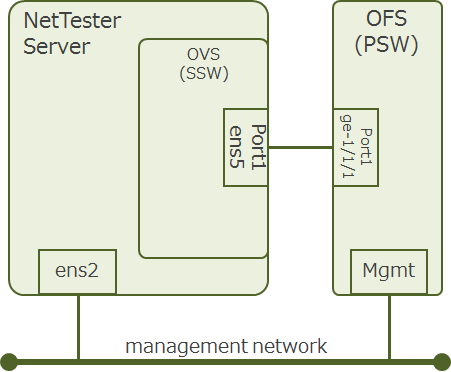
\includegraphics[scale=0.6]{img/nettester-deploy-baremetal.png}
 \caption{ベアメタル構成}
 \label{fig:nettester-deploy-baremetal}
\end{figure}

\paragraph{仮想マシン構成}
NetTesterサーバを仮想マシンとして構成する場合は
\figref{fig:nettester-deploy-vm}のようになる。管理ネットワークについては
ベアメタル構成の場合と同様にL2/L3でPSWとのコネクティビティがとれればよい。
NetTester(SSW)-PSW間の接続については、ホストOS側で物理ポート(リンク)を
NetTesterサーバ(VM)へ直結させる必要がある。SSW-PSW間はOFC(NetTester)によっ
て制御するため、ハイパーバイザ側ではL2以上の制御はおこなわない。パススルー
あるいはプロミスキャスモードで接続する。

\begin{figure}[h]
 \centering
 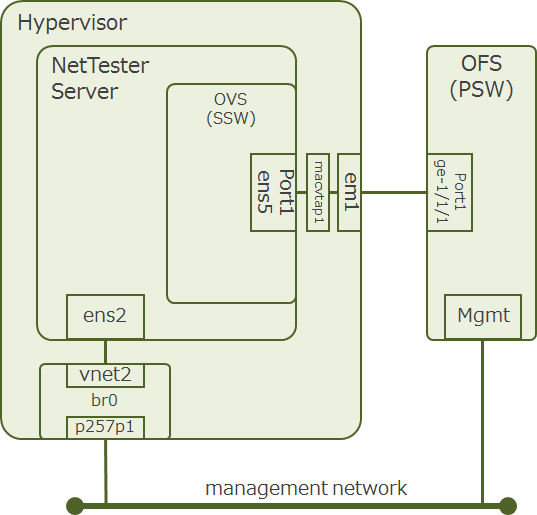
\includegraphics[scale=0.6]{img/nettester-deploy-vm.png}
 \caption{仮想マシン構成}
 \label{fig:nettester-deploy-vm}
\end{figure}

本プロジェクトは仮想マシン構成を採用した。PoCでは
\tabref{tab:server-spec}に示すサーバを使用している。SSW-PSW間接続では、
ハイパーバイザ(KVM Host)が持つ物理NICを直接仮想マシンに接続
(\code{macvtap/passthrough})させる(\lstref{lst:kvmconf-psw-port})。管理
ネットワークについては bridge 接続でよい(他のVMやハイパーバイザとL2で接
続する, \lstref{lst:kvmconf-mgmt-port})。

\begin{table}[hb]
 \centering
 \caption{NetTesterサーバ情報}
 \label{tab:server-spec}
 \begin{tabularx}{\linewidth}{l|X|X}
  \hline
  Host & OS & Virtualization \\
  \hline
  \hline
  \shortstack[l]{Hypervisor\\(KVM Host)}
    & \shortstack[l]{Ubuntu 14.04.5 LTS\\(GNU/Linux 3.16.0-30-generic x86\_64)}
    & \shortstack[l]{qemu-kvm/2.0.0+dfsg-2ubuntu1.25,\\libvirt/1.2.2-0ubuntu13.1.17} \\
  \hline
  \shortstack[l]{NetTester Server\\(VM)}
    & \shortstack[l]{Ubuntu 16.04.1 LTS\\(GNU/Linux 4.4.0-31-generic x86\_64)}
    & \\
  \hline
 \end{tabularx}
\end{table}

\begin{lstlisting}[language=xml,caption=PSW接続用ポート設定,label=lst:kvmconf-psw-port]
<interface type='direct'>
  <mac address='52:54:00:12:56:0e'/>
  <source dev='em1' mode='passthrough'/>
  <target dev='macvtap1'/>
  <model type='virtio'/>
  <alias name='net1'/>
  <address type='pci' domain='0x0000' bus='0x00' slot='0x05' function='0x0'/>
</interface>
\end{lstlisting}
\begin{lstlisting}[language=xml,caption=管理ポート設定,label=lst:kvmconf-mgmt-port]
<interface type='bridge'>
  <mac address='52:54:00:64:ee:38'/>
  <source bridge='br0'/>
  <target dev='vnet2'/>
  <model type='virtio'/>
  <alias name='net0'/>
  <address type='pci' domain='0x0000' bus='0x00' slot='0x02' function='0x0'/>
</interface>
\end{lstlisting}


  \subsection{NetTester Server のソフトウェア構成}
  \label{sec:nettester-server-software}

  % 必要なソフトウェア(package)とインストール
  % - 基本的なパッケージ
  %   - open vswitch
  %   - ruby, rubyenv
  %   - Git
  %   - Build-Essentials
  % - OSの設定
  %   - sudoers secure\_path

    \paragraph{NetTesterを使用するために必要なソフトウェア}
\nettester を使用するための必須ソフトウェアとPoCで使用したバージョンにつ
いて\tabref{tab:nettester-software-stack}に示す。使用するソフトウェアの
導入にあたっての注意事項を以下に示す。
\begin{itemize}
 \item \tabref{tab:nettester-software-stack}以外に必要な一般的な開発ツー
       ル等については Build Essential~\cite{build-essential-doc}などで導
       入しておく\footnote{\code{sudo apt install build-essential}}こと。
 \item NetTesterで使用するRuby package(gem)はbundlerで自動的にインストー
       ルされる。GemについてはNetTesterリポジトリ内 \code{Gemfile}等を参
       照すること。
 \item Rubyについてはrbenv~\cite{rbenv}などで複数のrubyバージョンを管理
       する環境でもよい。
 \item NetTesterはバックエンドで\code{ip}コマンドを使用してNetwork
       Namespaceの操作をおこなっている\footnote{正確にはNetTesterが利用
       しているTrema/Phutが\code{ip}コマンドを使用している。
       \ref{sec:phut_basics}節参照。}。このときroot権限が必要になり
       \code{sudo}を使用して実行する。\code{sudo}利用にあたって
       \code{PATH}まわりのエラーが発生する場合は\code{sudo}設定ファイル
       (\code{/etc/sudoers})の\code{secure\_path}設定を修正すること。
\end{itemize}

  \begin{table}[H]
   \centering
   \caption{NetTester Serverのソフトウェア構成}
   \label{tab:nettester-software-stack}
   \begin{tabularx}{\linewidth}{l|l|X}
    \hline
    Software & Version (PoC) & Notes \\
    \hline
    \hline
    OS (Linux) & \shortstack[l]{Ubuntu 16.04 (GNU/Linux 4.4.0),\\ \tabref{tab:server-spec}参照} & Linux Network Namespace が使用できること。 \\
    \cline{1-2}
    iproute2 & 4.3.0 & \\
    \hline
    ethtool & 4.5 & NIC オフロード機能操作 \\
    \hline
    Git & 2.7.4 & \\
    \hline
    Open vSwitch & 2.5.0 & SSWとして使用する。\tabref{tab:ofs-requirement}満たすこと。 \\
    \hline
    Ruby & 2.3.1p112 & 2.0以上が必要。2.3以上を推奨。\\
    \hline
   \end{tabularx}
  \end{table}

    \paragraph{Open vSwitch(SSW)の設定}
NetTesterサーバ上のソフトウェアスイッチは、NetTester起動時に都度
NetTesterが設定をおこなうため、事前に設定等をおこなう必要はない。
NetTesterを起動すると、\ref{sec:nettester-model-restriction}節に示した
DPIDでOpen vSwitchのブリッジが作成され、OFCとの接続設定がおこなわれる。

    \paragraph{NICのハードウェアオフロード機能操作}
    % trunkを使ってTCP通信するとおかしくなる – NetTester
    % https://3.basecamp.com/3088280/buckets/867009/todos/368843648
    % Netns Checksum Offload 機能実装 – NetTester
    % https://3.basecamp.com/3088280/buckets/867009/todos/370752297
NetTesterをつかったテストシナリオの実装・テスト実行にあたって、以下の条
件でテスト用ノードが生成しているTCPパケットのチェックサムが incorrect と
なり、正しく通信がおこなえないという事象がおきた。
\begin{itemize}
 \item テスト用ノードをテスト対象ネットワークに trunk port で接続させる
       (OVSでVLAN Tagの操作をおこなう)
 \item テストトラフィックとしてTCP通信をおこなう。
       \begin{itemize}
        \item SYN/FINフラグがついたトラフィックについては問題が発生しな
              い。(TCPの特定のフラグがついたパケットで問題がおきる。)
        \item ICMP通信については問題が発生しない。
       \end{itemize}
\end{itemize}

根本的な原因究明はできていないが、ワークアラウンドとして、NetTesterでテ
スト用ノード(Netns)を生成した際に、テスト用ノードへ接続するNIC(veth)で
チェックサム計算のハードウェアオフロードをオフにしてい
る~\cite{net-tester-pr7}。

  \subsection{テストシナリオ (net-tester/examples) のインストール}
  \label{sec:deploy-test-cenario}
  % 必要なソフトウェア(package)とインストール
  % - 基本的なパッケージ
  %   - テストシナリオでつかうもの (nc, dnsmasqなど)

  % テストシナリオで使うツール(package)の解決 – NetTester
  % https://3.basecamp.com/3088280/buckets/867009/todos/327898933

本プロジェクトでは、NetTester を使用したネットワークのテストシナリオを
\nettesterex として整備している。

テストシナリオをインストールする場合は\lstref{lst:install-scenario}の手
順を実行する。テストシナリオの中でNetTesterはテスト用ノード操作をおこな
う際に使用するツールのひとつとなるため、bundlerにより自動的にインストー
ルがおこなわれる。NetTester以外にテストシナリオ(Cucumberで記述)内で使用
するruby gemsについても、リポジトリ内\code{Gemfile}等で管理される。

\begin{lstlisting}[language=sh,caption=テストシナリオのインストール,label=lst:install-scenario]
git clone https://github.com/net-tester/examples.git
cd examples
bundle install --binstubs --path=vendor/bundle
\end{lstlisting}

このほかに、テストシナリオでは、NetTesterを使って生成・配置したテスト用
ノードの上で、さらにテストトラフィックを生成し end-to-end の通信状況を見
ていくためのツールが必要になる。PoCテストシナリオでは
\tabref{tab:tools-for-scenario}に示すツールを使用している。2017年1月時点
で、テストシナリオ内で使用する(bundlerで管理できるruby packageではない)
ツールについては統一して管理することはできておらず、別途手動で必要なツー
ルをインストールする必要がある。

\begin{table}[h]
 \centering
 \caption{PoCテストシナリオ内で使用するツール}
 \label{tab:tools-for-scenario}
 \begin{tabular}{l|l|l}
  \hline
  Tool(package) & Version(PoC) & テストシナリオ内での使いかた \\
  \hline
  \hline
  netcat(\code{nc}) & 1.105 & 汎用/簡易TCPサーバとして使用 \\
  dnsmasq & 2.75 & DNS通信テスト用の軽量DNSサーバとして使用 \\
  \hline
 \end{tabular}
\end{table}

  \subsection{NetTesterのインストール}

テストシナリオを中心にネットワークのテストを開発する場合は
\ref{sec:deploy-test-cenario}節のとおり、テスト・プロジェクト(リポジトリ)が
使用するツールのひとつとしてNetTesterが含まれる。

NetTesterを直接(単体で)使用して簡単なテスト操作を行なうこともできる。そ
うした場合には\lstref{lst:install-nettester}の手順でNetTester単体でのイ
ンストールをおこなう。

\begin{lstlisting}[language=sh,caption=NetTesterのインストール,label=lst:install-nettester]
git clone https://github.com/net-tester/net-tester.git
cd net-tester
bundle install --binstubs --path=vendor/bundle
\end{lstlisting}

 \section{基本的な使い方}
 \label{sec:basic-usage}

  \subsection{NetTesterが使用する環境変数}
  \label{sec:nettester-envvar}
  % 環境変数の設定
  % - ``DEVICE``
  %   - 調査:セグメントローカルの試験がとおらない – NetTester
  %     \url{https://3.basecamp.com/3088280/buckets/867009/todos/259184454}
  %   - ネットワークデバイスと dpid を rake に渡せるようにする – NetTester
  %     \url{https://3.basecamp.com/3088280/buckets/867009/todos/214833956}
  % - expectacle 関連についてはappendixにうつすか。

NetTesterは以下の2つの環境変数を使用する。
\begin{description}
 \item[\code{DEVICE}] NetTesterサーバ上で、SSW-PSW間を接続するために使用
            するNICを指定する。
 \item[\code{DPID}] 物理OpenFlowスイッチ(PSW)のDatapath IDを指定する。
\end{description}

\figref{fig:nettester-deploy-vm}の場合は\code{DEVICE=ens5}、
\code{DPID=0x1}となる。テストシナリオ(NetTester Examples)では\code{rake}
により複数のテストシナリオの一括実行(回帰テスト)を実行できる。
\code{rake}実行時には次のように環境変数を指定して回帰テストを実行する。
\begin{lstlisting}
rake DEVICE=ens5 DPID=0x1 cucumber
\end{lstlisting}

この他にも、実際のテストシナリオ実行の際に、テスト対象ネットワーク機器操
作のために使うツール(\ref{sec:expectacle}節)でも環境変数を使用するので注
意すること。

  \subsection{NetTester APIの基礎}
  \label{sec:nettester-api-basics}
  % NetTesterでad-hocなテスト作業を拡張する - Qiita
  % \url{http://qiita.com/corestate55/items/d6a8cdc03de09a46877c}

NetTesterを使った処理の基本的な流れと、APIの基本的な使用方法を例をもとに
解説する。

\paragraph{サンプル環境構成}

いま\figref{fig:nettester-basic-example}のように、テスト対象ネットワーク
にあるふたつのL2スイッチ(L2SW)に、それぞれ1台ずつテスト用ノードを接続し
てテスト作業をおこなうことを想定する。このとき、テスト用ノードの生成およ
び配置・接続はNetTesterを使用しておこなう。また、テスト用ノードで実施す
るテスト作業はPry~\cite{pry}を使用してad-hocに(手動で)実施する。

これをNetTester APIを用いて実装すると
\lstref{lst:nettester_basic_example}のようになる\footnote{このスクリプト
は解説用にパラメタ設定などを冗長に記載している。実際にテストシナリオ等を
実装する場合は、より無駄のない形で記述することができる
(\ref{sec:test-parameter-management}節参照)。}。
% TODO: FactoryGirlの話とかへの参照をいれたい

\begin{figure}[h]
 \centering
 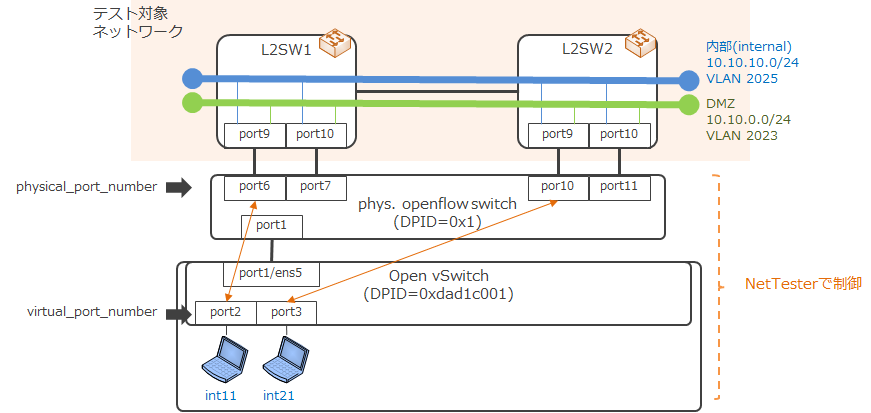
\includegraphics[scale=0.75]{img/nettester-basic-example.png}
 \caption{NetTester利用例(構成図)}
 \label{fig:nettester-basic-example}
\end{figure}

\begin{lstlisting}[caption=NetTester基礎,label=lst:nettester_basic_example]
#!/usr/bin/env ruby
# frozen_string_literal: true

require 'net_tester'
require 'pry'

# parameter definition
nwdev = 'ens5'
pss_dpid = 0x1
mac_base = '00:ba:dc:ab:1e:'

p '# run net_tester'
NetTester.run(network_device: nwdev,
              physical_switch_dpid: pss_dpid)
p '# wait ssw/psw connection'
sleep 10

p '# Create host11 in internal segment (ip:10.10.10.7, vlan:2025)'
host11 = NetTester::Netns.new(name: 'host11',
                              mac_address: mac_base + '01',
                              ip_address: '10.10.10.7',
                              netmask: 24,
                              gateway: '10.10.10.254',
                              virtual_port_number: 2,
                              physical_port_number: 6,
                              vlan_id: 2025)

p '# Create host21 in internal segment (ip:10.10.10.9, vlan:2025)'
host21 = NetTester::Netns.new(name: 'host21',
                              mac_address: mac_base + '02',
                              ip_address: '10.10.10.9',
                              netmask: 24,
                              gateway: '10.10.10.254',
                              virtual_port_number: 3,
                              physical_port_number: 10,
                              vlan_id: 2025)

# into pry console
binding.pry

# cleanup
NetTester.kill
\end{lstlisting}

    \paragraph{NetTesterによるテスト操作の流れ}
NetTesterを使ったネットワークのテスト操作は次のステップで実装される。
\begin{enumerate}
 \item NetTesterを起動する
       \begin{itemize}
        \item \verb|NetTester.run| (引数については
              \ref{sec:nettester-envvar}節参照)
        \item 起動すると、SSWの設定とOFCの起動をおこなう。
              \lstref{lst:nettester_basic_example}ではOFC起動後にSSW/PSW
              の接続を待つために\code{sleep}を設定している。
       \end{itemize}
 \item NetTesterでテスト用ノードを生成する
       \begin{itemize}
        \item \verb|NetTester::Netns.new| によって Network Namespace を
              使ったテスト用ノードを生成する。(詳細については
              \ref{sec:phut_basics}節参照)
        \item 生成と同時にテスト対象ネットワークへの配置(パッチ接続)をお
              こなう。引数\verb|virtual_port_number|および
              \verb|physical_port_number|は「パッチ」の両端点となるポー
              ト番号をあらわしている。ここで指定された端点情報をもとに、
              NetTesterはOpenFlowスイッチ(PSW, SSW)にフロールールを設定
              する。
        \item \figref{fig:nettester-basic-example}で、L2SW側のテスト用ノー
              ド接続ポートはTrunk Port (vlan tagged port)になっている。
              そのため、\code{vlan}オプションを指定して、テスト用ノード
              が生成するトラフィックにVLAN Tagを追加することを指定してい
              る。
       \end{itemize}
 \item 生成したテスト用ノード上で作業をおこなう
       \begin{itemize}
        \item \verb|NetTester::Netns#exec| (後述)
       \end{itemize}
 \item NetTesterを終了する
       \begin{itemize}
        \item \verb|NetTester.kill|
        \item NetTesterが生成したSSW, テスト用ノードなどを削除する。テス
              ト用ノード(\verb|NetTester::Netns|)の実態は network
              namespace であるため、NetTsterプロセスが消去されてもOS上に
              設定が残る。適切な終了(削除)処理がおこなわれない場合、OS上
              にこれらの設定が残りつづけてしまう(他のテストシナリオ実行
              時に同名のnamespaceを作成しようとするとエラーになる)ため注
              意が必要である。
       \end{itemize}
\end{enumerate}

テスト用ノード上での操作については、このスクリプトではpryによるインタラ
クティブシェル上での操作となる。生成したテスト用ノード上(テスト用ノード
のnamespace上)でコマンドを実行することでテスト作業をおこなう。テスト用ノー
ド上でのコマンド実行には\verb|NetTester::Netns#exec|を使用する。たとえば
次のような操作を実施することができる。
\begin{lstlisting}[language=sh,title=テスト作業例]
[31] pry(main)> puts host11.exec("ping -c3 #{host21.ip_address}")
PING 10.10.10.9 (10.10.10.9) 56(84) bytes of data.
64 bytes from 10.10.10.9: icmp_seq=1 ttl=64 time=0.514 ms
64 bytes from 10.10.10.9: icmp_seq=2 ttl=64 time=0.336 ms
64 bytes from 10.10.10.9: icmp_seq=3 ttl=64 time=0.311 ms


--- 10.10.10.9 ping statistics ---
3 packets transmitted, 3 received, 0% packet loss, time 1998ms
rtt min/avg/max/mdev = 0.311/0.387/0.514/0.090 ms
=> nil
[32] pry(main)>
\end{lstlisting}

    \paragraph{Pry応用}
\lstref{lst:nettester_basic_example}を拡張してテスト用ノードを多数配置し、
PryとNetTesterを併用してインタラクティブにテスト作業をおこなうといった応
用もできる。このような応用については本書では扱わない。別途資
料~\cite{nettester-pry}を参照すること。

% TODO: ここで含めるか?
% - コマンド実行/並列コマンド実行?

%%% Local Variables:
%%% mode: yatex
%%% TeX-master: "main.tex"
%%% End:

%% -*- coding: utf-8-unix -*-

\chapter{PoCターゲット設計}
\label{chap:poc-target-design}

PoCとしてユースケース実証実験をおこなう際に設定したPoCシナリオ(状況設定)、
PoC環境について解説する。

% TODO: ここにたどりつく前段階の検討のはなしをいれるか?
% アーキテクチャ検討_20160617.pptx
% https://drive.google.com/open?id=0B2eRR_JxYJA5RXdPTzVLU1M4RzQ

 \section{PoCの概要}
 \label{sec:poc-overview}

 % なんのために、どういったテストをおこなうのか。
 % そもそものPoCの考え方のまとめ・整理

 % 障害報告ストーリー – NetTester
 % \url{https://3.basecamp.com/3088280/buckets/867009/documents/151143879}
 % どういったサービス上のトラブルを検出したいとおもったのか? (ユースケース例)
 % 技術的にやりたいこと:  静的なテスト/動的なテスト

 \subsection{PoCの目的}
 \label{sec:poc-purpose}

\lopjc では network namespace によるテスト用ノード生成とOpenFlowスイッチ
による配置(パッチ)という、\tabref{tab:test-functions}のNo.3,4に相当する
技術の基礎検証を実施した。本プロジェクトでは、それらの基礎技術をもとに
NetTesterを実装し、実際のテスト(ユースケース)としてどういったテストが自
動化可能か(\tabref{tab:test-functions}, No.5)を中心に実証していく。テス
トのユースケースとして、静的なふるまい・動的なふるまいのふたつの観点でテ
ストシナリオの実装を進める(\ref{sec:behavior-test}節)。

  \subsection{PoCターゲットユースケース検討}
  \label{sec:poc-usecase-discuss}

ネットワークテストのユースケースとしてとして\tabref{tab:test-usecases}の
ような事例について検討した。

\tabref{tab:test-usecases}の事例をもとに、汎用性があり、かつ「テストの自
動化」という観点で技術的に基礎となる機能を盛り込めるユースケースとして、
以下の2ケースを選択した。いずれもテスト自動化の有効性を出しやすい条件を
満たす(頻繁にくりかえしおこなう・複雑度が高く人によるレビュー等でのミス
の発見が難しい・従来は人力にたよっており自動化が難しい)という観点で選択
している。
\begin{itemize}
 \item FWのパケットフィルタポリシ運用
       \begin{itemize}
        \item 「静的なふるまい」の代表例として選択。
        \item FWポリシ管理(通信制御ポリシ管理)は、パターン数(ルール)が多
              く、順序の依存関係など複雑度の高い操作が求められるため。ま
              た日々の変更頻度が高く、運用管理コストの高い事例であるため。
        \item 特にアプリケーションレイヤ(L7)を検査するDPI機能を持つFWの
              テストは単純なL3/L4のツールでは自動化が難しい動作であるた
              め。
       \end{itemize}
 \item 冗長化構成FWのリンク障害試験
       \begin{itemize}
        \item 「動的なふるまい」の代表例として選択。(最も基本的な「動的
              なふるまい」の例としての物理トポロジ(物理リンク)操作。)
        \item 一般的に、FW(ハードウェアアプライアンス)はその機能や性能上
              の理由から製品ごとに固有のアーキテクチャを持つ。製品機能や
              性能を維持しつつ、FWを経由するセッションなどの情報(状態)を
              クラスタとして保持するために、FWのクラスタ化では製品ごと固
              有の機能実装を持つ。そのため、製品ごとに固有の機能やバグが
              あり、実際本番環境で使用する実機(ハードウェア)を使用したテ
              ストが重要になる。
        \item クラスタ化されたFWのフェイルオーバー/フェイルバックはステー
              トフルな動作となり、初期状態の設定、指定された手順を実行し
              てネットワークの状態を遷移させていくオペレーションが必要と
              なる。また、状態遷移中の動作を複数並列してチェックしていく
              必要がある。いずれも従来は複数人で作業することでおこなって
              いたものだが、複数人による作業は全体の動作などが掴みにくい
              という問題があった。
       \end{itemize}
\end{itemize}

\begin{table}[hb]
 \centering
 \caption{テストユースケース案}
 \label{tab:test-usecases}
 \begin{tabularx}{\linewidth}{p{10em}|X}
  \hline
  ユースケース & 詳細(事例) \\
  \hline
  \hline
  ネットワーク移設時の通信不能 & ある拠点から他のDCへのシステム移設の際、現行システムのIPを継続するためにL2延伸をおこなっていたが、上流側ネットワークでの経路消失により通信ができなくなった。 \\ \hline
  FW通信誤許可 & 外部からhttpでアクセス不能なはずのシステムについて、実際には外部からのhttpでのアクセスが許可されていた。 \\ \hline
  システム拡張時の通信不安定 & システムの拡張時にL2ループが発生し通信が不安定になった。 \\ \hline
  FWの再起動による通信障害 & Active/Standby構成のFWでStandby側が再起動したときに、Active側が機能停止・冗長構成の情報交換ができず通信が停止した。\\ \hline
  通信遅延の発生、ネットワークのスローダウン & L3スイッチのリソース(メモリ・TCAM)枯渇による重大なネットワーク性能低下、通信遅延が発生した。 \\ \hline
  経路制御設定ミスによるアクセス不能 & サーバリプレースによりシステム側のIPアドレスが変更となった際、一部機器でルーティング追加作業が漏れていたためにシステムへアクセス不能となった。 \\ \hline
  FW のリプレース & 古いFW機器(ハードウェア)を新しい世代の機器にリプレースする際、既存のルールのコンバートやインポートに問題があり一部の通信が停止した。 \\ \hline
  FW フィルタ(ポリシ)のミスチェック & パケットフィルタはルール(ポリシ)としては設定されているが、ルール作成者の認識違いやミスなどで最終的に実現したいポリシになっておらず、必要な通信の遮断・不要な通信の透過が発生してしまった。 \\
  \hline
 \end{tabularx}
\end{table}

  \subsection{PoC方針}

  % TODO みなおし -> https://drive.google.com/open?id=0B2eRR_JxYJA5Vm1Dd0dJRGdjWU0
ここまでで既にいくつか方針をあげているが、あらためてPoCの実施方針をまとめる。
\begin{itemize}
 \item 本PoCで実施すること
       \begin{itemize}
        \item テストシステムの機能・特定の自動化実装ではなく、「テストと
              して実行可能なユースケース」に注目する。
        \item ネットワークテストの基本的な考えかたとして「静的なふるまい
              のテスト」「動的なふるまいのテスト」の観点で実際のテストシ
              ナリオを実装する。
        \item 「ネットワークのふるまい」として、end-to-endの通信の実現可
              否に着目する。ネットワークの設計・内部構造・使用している機
              材に関わらず、ネットワークとしてどういった通信が実現される
              べきか、という要求とそのテストに注目する。これは、ネットワー
              クの利用者から見たネットワークに対する期待(要求)、あるいは
              ネットワーク(サービス)提供者の視点から見たネットワークに対
              する期待\footnote{サービス提供者として、ネットワーク利用者
              にどういったサービスが提供できなければいけないか。}を確認
              することである。
       \end{itemize}
 \item 本PoCで実施しないこと
       \begin{itemize}
        \item 「できないこと」のテスト: 利用者あるいはサービス提供者の視
              点では、ネットワーク上「できてはいけないこと」の要求がある。
              例えば、隣接する他者顧客環境と通信ができてはいけない、など。
              本PoCはまず利用者に対して最低限提供すべきサービス(「できな
              ければいけないこと」)についてのテストに焦点をあてる。
        \item 非機能要件のテスト(性能・拡張性・冗長性): 上記のとおり、本
              PoCではネットワークテスト(ユースケース)の実現可否、機能的
              な実現性に注目する。そのため、性能や拡張性などについては考
              慮せず、ユースケースを実現可能な最低限のシステム構成・実装
              をとることを方針としている。
       \end{itemize}
\end{itemize}

 \section{PoCターゲットの設定}

  \subsection{登場人物}
  \label{sec:poc-casting}

PoCにあたって\figref{fig:poc-situation}のように登場人物を設定した。
\begin{itemize}
 \item ヨーヨーダイン社\footnote{架空の企業名\cite{yoyodyne}}
       \begin{itemize}
        \item タジマックス通信工業社と共同でソフトウェア開発をおこなって
              いる。
        \item 社内ネットワークの新規構築をおこなうにあたり、ネットワーク
              の設計・構築についてもタジマックス通信工業社に発注すること
              になった。
       \end{itemize}
 \item タジマックス通信工業社\footnote{架空の企業名, プロジェクトメンバ
       の氏名から。}(以降 \tj )
       \begin{itemize}
        \item ソフトウェア開発および情報システム基盤の設計・構築などをお
              こなっている。
        \item ヨーヨーダイン社の社内ネットワーク設計構築を受注している。
       \end{itemize}
\end{itemize}

\begin{figure}[h]
 \centering
 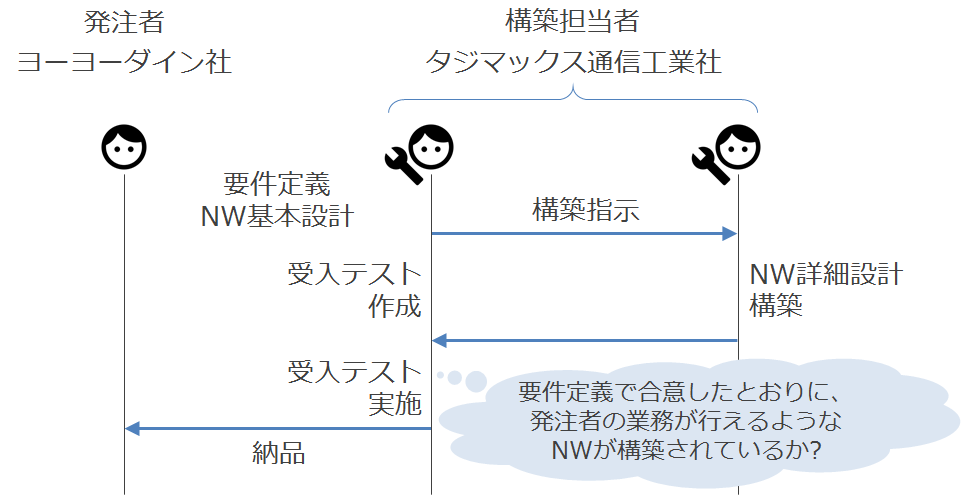
\includegraphics[scale=0.5]{img/poc-situation.png}
 \caption{PoC設定: 登場人物の位置付け}
 \label{fig:poc-situation}
\end{figure}

以降、ネットワークのテストシナリオについては、\tj 社員がテストをする視点
をとる。(\tj 社員がネットワークの設計・構築をおこない、\yo へ納入する前
に、\yo が業務をおこなう上で実現したいこと、\yo の要求すべてが問題なく実
現できているかどうかをテストする。)

\ref{chap:poc-scenario-dev}章で実際のテストシナリオ実装について解説する
が、PoCでは \tj 社員に相当するメンバとして次のように設定した。
\begin{itemize}
 \item ネットワークの要件定義・基本設計を行なうネットワークエンジニア
 \item 決められたネットワーク要求に基づいてネットワークの構築をおこなう
       ネットワークエンジニア
 \item 決められたネットワーク要求に基づいてテストシナリオの実装・実行を
       おこなうソフトウェアエンジニア
\end{itemize}

ネットワークエンジニア担当のPoCメンバは、プログラミングの知識があり、テ
ストシナリオの実装やテストシナリオ実行時に発生した問題のトラブルシュート
が可能なスキルを持つ。テストシナリオ実装をおこなうソフトウェアエンジニア
については、ネットワーク(TCP/IP, Ethernet)の基本的な知識はあり、ネットワー
ク要件やそれに応じてどのようなテストを実行すればよいかを考えることができ
るが、ネットワーク機器の設定などを実際には(ほとんど)おこなったことのない
メンバを設定している。

  \subsection{サービス要件定義}

以下、PoC上の状況設定をおこなう。なお、PoCを複雑化させないため、原則
L1-L4までの機能的な要件設定とし、(可用性を除く)非機能要件や主要な要件に
付随する業務上の要求(アクセスログ取得等セキュリティ観点の要求など)は設定
していない。

    \paragraph{機能要件}
\yo および \tj が共同開発をおこなうための機能要件は次のようになる
\footnote{平成25年度のネットワークスペシャリスト試験の問題\cite{h25nwsp}
をもとに、架空の中小企業ネットワークとして設定している。}。
\begin{itemize}
 \item \yo は社内に開発環境を持つ。開発環境は社内からのみアクセス可能と
       する。
 \item \tj はインターネット経由で \yo 社内にアクセスし、開発環境を共用し
       て \yo との開発業務をおこなう。
       \begin{itemize}
        \item \tj からのアクセスはセキュアな通信方法をとること(通信を暗
              号化すること)
        \item \tj からのアクセスについて個人単位での認証・アクセスコント
              ロールができること。
       \end{itemize}
 \item \yo が社内外に提供するサービスは、インターネット環境に直接は設置
       せず、上流ネットワークで \yo によるL4(以上)のアクセス制御を行なう
       こと。
 \item インターネット側から \yo 社内への通信を許可しない。(\yo がインター
       ネット側に提供するサービスを除く。)
\end{itemize}

    \paragraph{可用性}

ネットワークの可用性については次のように設定する。
\begin{itemize}
 \item インターネット回線の冗長化はおこなわない\footnote{PoC設定上の都合。
       障害試験ポイントとしてNW機器(FW)にのみ注目する。}。
 \item 社内では中核をなすNW機器の冗長化をおこなう。(機器メンテナンス作業
       や障害発生時の \tj 開発業務継続のため。)
\end{itemize}

 \section{環境構成(Target Network)}
 % - L2/L3, Management network (VR/VRFとout-of-band設定)
 % - FWの冗長化設定:
 %        - active/passive, passiveはパケット転送しない
 %        - tcp session state を同期する
 %        - 状態監視するインタフェースの設定、自動復旧設定とする
 % - FWのフィルタ設定:
 %        - 原則L3/L4でのフィルタ
 %        - tcp state をみる
 %        - DNSについてはL7(DPI)でフィルタする

 % - IPアドレス表 \url{https://drive.google.com/open?id=1v0ecUjUql3cxVMP8gvLyq4T9PEIeUeyMT_-9YrR4l0A}

  \subsection{論理ネットワーク設計}
  \label{sec:logical-nw-design}

  \paragraph{利用者要件}
\tj は \yo とのネットワーク要件検討をもとに、
\figref{fig:poc-env-logical}・\tabref{tab:ip-list}のようなネットワークを
構築することとした。

\begin{itemize}
 \item \yo ネットワークは、外部(社外/インターネット)・DMZ・内部(社内)の
       セキュリティゾーンに分割する。
 \item 外部(external)ゾーン: インターネット接続用の固定IPセグメントをひとつ持ち、
       インターネット経由で外部へのサービスを提供できるようにする。
       \begin{itemize}
        \item グローバルIPアドレスは外部ゾーンのみで使用する。DMZおよび
              内部ゾーンではプライベートIPアドレスを使用する。社外(イン
              ターネット)との必要な通信についてのみ、外部ゾーン境界(FW)
              でNATをおこなう。
       \end{itemize}
 \item DMZゾーン: 外部に公開するサービスと内部に公開するサービスの中継を
       おこなう。
       \begin{itemize}
        \item SSL VPNサーバ: \tj との共同開発業務のために、インターネッ
              ト経由で \tj からのリモートアクセスを受け付ける。\tj VPNク
              ライアントはVPN接続後、VPNサーバから割り当てられたDMZ内IP
              を使用して内部ゾーンの開発環境にアクセスする。
        \item DNSサーバ: \yo 内部向けに提供する名前解決・サービス
       \end{itemize}
 \item 内部(internal)ゾーン: 社内のみ利用可能な開発系サーバおよび社員(開
       発用PC等)を設置する。
       \begin{itemize}
        \item 開発環境として、資産管理サーバ(Git)・内部テストサーバ
              (Telnet/Jenkins)を起く。
       \end{itemize}
 \item アクセスポリシとして、原則、内部--外部ゾーン間の通信はおこなえな
       いものとする。ただし、現状は内部ゾーン内機器からのNTPおよび
       HTTP/HTTPS通信に関しては直接外部ゾーンへ通すことを許可する
       \footnote{\tj は、\yo NW規模およびセキュリティポリシを検討した結
       果、現時点ではProxyサーバ導入をおこなわないものとした。}。
\end{itemize}

なお、\tj の設計・構築範囲は \yo ネットワークである。\tj ネットワークに
ついてはPoCの対象には含まれない。

\begin{figure}[h]
 \centering
 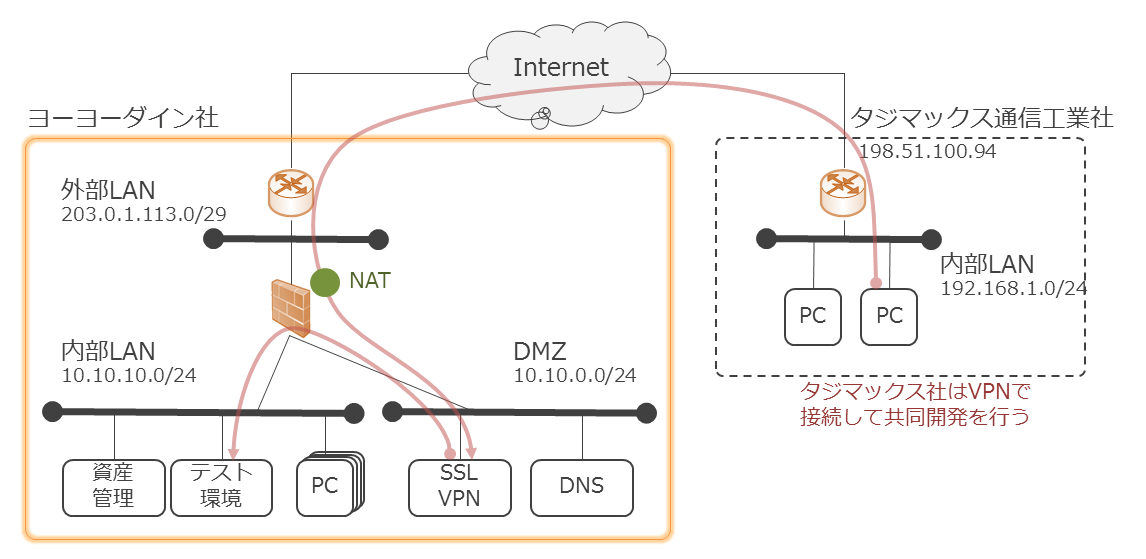
\includegraphics[scale=0.5]{img/poc-env-logical.png}
 \caption{PoC環境: 論理構成図}
 \label{fig:poc-env-logical}
\end{figure}

\begin{table}[h]
 \centering
 \caption{セグメント/IPアドレス一覧}
 \label{tab:ip-list}
 \begin{threeparttable}
  \begin{tabular}[t]{l|l|r|l}
   \hline
   Zone/Segment & IP Subnet & Local Host\tnote{1} & Host \\
   \hline
   \hline
   外部 & 203.0.113.0/29 & 0 & [Network] \\ \cline{3-4}
   & & 1 & Router \\ \cline{3-4}
   & & 2 & Firewall \\ \cline{3-4}
   & & 5 & SSLVPN ( \tj 社VPNアクセス) \\ \cline{3-4}
   & & 6 & NAPT (内部/DMZからInternetへのアクセス) \\ \cline{3-4}
   & & 7 & [Broadcast] \\ \hline
   DMZ & 10.10.0.0/24 & 0 & [Network] \\  \cline{3-4}
   & & 1 & Firewall (default gateway) \\ \cline{3-4}
   & & 10 & DNSサーバ \\ \cline{3-4}
   & & 11 & SSLVPNサーバ \\ \cline{3-4}
   & & 128-254 & SSLVPN Client IP Pool \\ \cline{3-4}
   & & 255 & [Broadcast] \\ \hline
   内部 & 10.10.10.0/24 & 0 & [Network] \\ \cline{3-4}
   & & 1 & 資産管理サーバ \\ \cline{3-4}
   & & 2 & テスト環境サーバ \\ \cline{3-4}
   & &  & 開発用PC \\ \cline{3-4}
   & & 254 & Firewall (default gateway) \\ \cline{3-4}
   & & 255 & [Broadcast] \\
   \hline
  \end{tabular}
  \begin{tablenotes}
   \footnotesize
   \item[1] 第4オクテット
  \end{tablenotes}
 \end{threeparttable}
\end{table}

    \paragraph{管理者要件}
ネットワークや各種サービスを運用・管理するための要求を以下のように設定する。
\begin{itemize}
 \item サーバ管理アクセス: 内部/DMZゾーンにおかれるサーバについては、\yo
       開発者が管理者を兼任しており、内部ゾーンから直接リモートアクセス
       することで運用・管理作業をおこなう。(in-band management)
 \item ネットワーク管理アクセス: ネットワーク機器の運用管理については、
       構築した \tj 社員をおくことを想定し、\yo ネットワークとは分離した
       設計とする。詳細については\ref{sec:mgmt-and-tester-nw}節参照。
\end{itemize}

  \subsection{通信要件}
  \label{sec:network-requirements}

利用者要件および管理者要件をふまえて、ネットワークで提供する通信要件は
\tabref{tab:poc-requires-yo-int}・\tabref{tab:poc-requires-yo-dmz}・
\tabref{tab:poc-requires-etc} のようになる。

\begin{landscape}
 \begin{table}[h]
  \centering
  \caption{PoC 通信要件(ヨーヨーダイン社内部セグメント起点)}
  % No.1-12
  \label{tab:poc-requires-yo-int}
  \begin{threeparttable}
   \begin{tabularx}{\linewidth}{c|X|X|X|X|X|X|X}
\hline
No. & ポリシ & アプリケーション & \multicolumn{2}{|l|}{Source IP} & \multicolumn{2}{l|}{Destination IP} & Destination Port \\
\hline
\hline
1 & PC→開発環境 & Git & PC & 10.10.10.0/24 & 資産管理サーバ & 10.10.10.1 & tcp/11000 \\ \hline
2 & PC→開発環境 & Telnet & PC & 10.10.10.0/24 & テスト環境サーバ & 10.10.10.2 & tcp/23 \\ \hline
3 & PC→開発環境 & Jenkins & PC & 10.10.10.0/24 & テスト環境サーバ & 10.10.10.2 & tcp/13000 \\ \hline
4 & PC→開発環境 & サーバ管理: ssh & PC & 10.10.10.0/24 & 資産管理サーバ & 10.10.10.1 & tcp/22,80,443 \\ \hline
5 & PC→開発環境 & サーバ管理: ssh & PC & 10.10.10.0/24 & テスト環境サーバ & 10.10.10.2 & tcp/22,80,443 \\ \hline
6 & PC→DNSサーバ & DNS Query & PC & 10.10.10.0/24 & DNSサーバ & 10.10.0.10 & tcp,udp/53 \\ \hline
7 & PC→Internet & Web browsing & PC & 10.10.10.0/24 & Internet & ANY & tcp 80,443 \\ \hline
8 & PC→Internet & NTP Query & PC & 10.10.10.0/24 & Internet & ANY & udp/123 \\ \hline
9 & PC→DNSサーバ & 応答確認: ping/traceroute & PC & 10.10.10.0/24 & DMZ & 10.10.0/24 & icmp \\ \hline
10 & PC→Internet & 応答確認: ping/traceroute & PC & 10.10.10.0/24 & Internet & ANY & icmp \\ \hline
11 & PC→DNSサーバ & サーバ管理: ssh & PC & 10.10.10.0/24 & DNSサーバ & 10.10.0.10 & tcp/22 \\ \hline
12 & PC→SSLVPNサーバ & サーバ管理: ssh, webui & PC & 10.10.10.0/24 & SSLVPNサーバ & 10.10.0.11 & tcp/22,80,443 \\ \hline
   \end{tabularx}
   \begin{tablenotes}
    \footnotesize
    \item ヨ社: ヨーヨーダイン社
    \item タ社: タジマックス通信工業社
   \end{tablenotes}
  \end{threeparttable}
 \end{table}
\end{landscape}

% AP1 : Git
% AP2 : Telnet
% AP3 : Jenkins

\begin{landscape}
 \begin{table}[h]
  \centering
  \caption{PoC 通信要件(ヨーヨーダイン社DMZセグメント起点)}
  % No.13-24
  \label{tab:poc-requires-yo-dmz}
  \begin{threeparttable}
   \begin{tabularx}{\linewidth}{c|X|X|X|X|X|X|X}
\hline
No. & ポリシ & アプリケーション & \multicolumn{2}{|l|}{Source IP} & \multicolumn{2}{l|}{Destination IP} & Destination Port \\
\hline
\hline
13 & DMZ→Internet & package update (web) & DMZ内サーバ & 10.10.0.0/25 & Internet & ANY & tcp/80,443 \\ \hline
14 & DNSサーバ→DNS Query & 上位DNSへのクエリ & DNSサーバ & 10.10.0.10 & Internet & ANY & tcp,udp/53 \\ \hline
15 & DMZ→DNSサーバ & DNS Query & DMZ内サーバ & 10.10.0.0/25 & DNSサーバ & 10.10.0.10 & tcp,udp/53 \\ \hline
16 & DMZ→NTP & NTP Query & DMZ内サーバ & 10.10.0.0/25 & Internet & ANY & udp/123 \\ \hline
17 & PC→DNSサーバ & ヨ社内部 & PC & 10.10.10.0/24 & DNSサーバ & 10.10.0.10 & tcp,udp/53 \\ \hline
18 & PC→DMZ & サーバ管理: ssh & PC & 10.10.10.0/24 & DMZ内サーバ & 10.10.0.0/25 & tcp/22,80,443 \\ \hline
19 & VPNPOOL→開発環境 & Git & DMZ VPN Pool & 10.10.0.128/25 & 資産管理サーバ & 10.10.10.1 & tcp/11000 \\ \hline
20 & VPNPOOL→開発環境 & Telnet & DMZ VPN Pool & 10.10.0.128/25 & テスト環境サーバ & 10.10.10.2 & tcp/23 \\ \hline
21 & VPNPOOL→開発環境 & Jenkins & DMZ VPN Pool & 10.10.0.128/25 & テスト環境サーバ & 10.10.10.2 & tcp/13000 \\ \hline
22 & DMZ→Internet & 応答確認: ping/traceroute & DMZ内サーバ & 10.10.0.0/25 & Internet & ANY & icmp \\ \hline
23 & DMZ→ヨ社内部 & 応答確認: ping/traceroute & ヨ社内部 & 10.10.10.0/24 & DMZ内サーバ & 10.10.0.0/25 & icmp \\ \hline
24 & ヨ社内部→DMZ & 応答確認: ping/traceroute & DMZ内サーバ & 10.10.0.0/25 & ヨ社内部 & 10.10.10.0/24 & icmp \\ \hline
   \end{tabularx}
   \begin{tablenotes}
    \footnotesize
    \item ヨ社: ヨーヨーダイン社
    \item タ社: タジマックス通信工業社
   \end{tablenotes}
  \end{threeparttable}
 \end{table}
\end{landscape}

\begin{landscape}
 \begin{table}[h]
  \centering
  \caption{PoC 通信要件(Internet/タジマックス社セグメント起点)}
  % No.25-28(Internet), No.29-30(タ社)
  \label{tab:poc-requires-etc}
  \begin{threeparttable}
   \begin{tabularx}{\linewidth}{c|X|X|X|X|X|X|X}
\hline
No. & ポリシ & アプリケーション & \multicolumn{2}{|l|}{Source IP} & \multicolumn{2}{l|}{Destination IP} & Destination Port \\
\hline
\hline
26 & Internet→外部 & 応答確認: ping/traceroute & Internet & ANY & Router & 203.0.113.1 & icmp \\ \hline
27 & Internet→外部 & 応答確認: ping/traceroute & Internet & ANY & Firewall & 203.0.113.2 & icmp \\ \hline
28 & 外部→Internet & 応答確認: ping/traceroute & ヨ社外部 & 203.0.113.0/29 & Internet & ANY & icmp \\ \hline
29 & PC→ヨ社VPN & SSLVPN & タ社(Global) & 198.51.100.94 & SSLVPNサーバ & 203.0.113.5 & tcp/80,443 \\ \hline
30 & PC→ヨ社VPN & 応答確認: ping/traceroute & タ社(Global) & 198.51.100.94 & SSLVPNサーバ & 203.0.113.5 & icmp \\ \hline
   \end{tabularx}
   \begin{tablenotes}
    \footnotesize
    \item ヨ社: ヨーヨーダイン社
    \item タ社: タジマックス通信工業社
   \end{tablenotes}
  \end{threeparttable}
 \end{table}
\end{landscape}

  \subsection{物理ネットワーク設計}
  \label{sec:physical_nw_design}

    \paragraph{物理設計の基本的な考えかた}
論理ネットワーク設計(\ref{sec:logical-nw-design}節)をもとに、物理ネット
ワーク設計を\figref{fig:poc-env-physical}のようにした。使用した機器の詳
細については\tabref{tbl:device-list}参照。
\begin{itemize}
 \item セキュリティゾーンおよびゾーン間通信ポリシはFirewallによっておこ
       なう。
       \begin{itemize}
        \item 外部: WAN/Untrust Zone
        \item DMZ: DMZ Zone
        \item 内部: LAN/Trust Zone
       \end{itemize}
 \item 外部ゾーンはFW上流側L3SWで収容する。L3SWはinternet境界(キャリア回
       線終端)である。
 \item 内部ゾーンおよびDMZはL2SW1/L2SW2で収容する。物理リンクは共有し、
       VLANによって論理的に分離する。
\end{itemize}

管理系ネットワークについてはサービス系ネットワークと分離する
(\ref{sec:mgmt-and-tester-nw}節)。

    \paragraph{冗長性}

社内ネットワーク冗長化の要求からFirewallを冗長化する。
\begin{itemize}
 \item FirewallはActive/Passive方式とする。障害が発生していない場合はFW1
       が通常Activeとなり、トラフィックの転送をおこなうものとする。
 \item Active側FW(FW1)のもつすべてのリンクについて、いずれかひとつでもリ
       ンクダウンが発生した場合に自動的に処理をPassive側(FW2)へ切り替え
       る。
 \item 切替のトリガとなったリンクダウンが復旧し、FW1のすべてのリンクが正
       常になった場合は、トラフィック処理をFW1へ切り戻す。
 \item ステートフルフェイルオーバー: FW1/FW2は常に処理しているセッション
       の情報を同期し、切替・切り戻しが発生した際でも処理中のトラフィッ
       ク(セッション)を維持する。
\end{itemize}

    % \paragraph{パケットフィルタ}
    % DNSのテスト作る – NetTester
    % https://3.basecamp.com/3088280/buckets/867009/todos/301325453
    % SSGでDNS DPIするみたいな記述はみあたらない。
    % どう書くか...

% Firewall では基本的にL3/L4のパケットフィルタをおこなう(ステートフルイン
% スペクション可能)。

\begin{figure}[h]
 \centering
 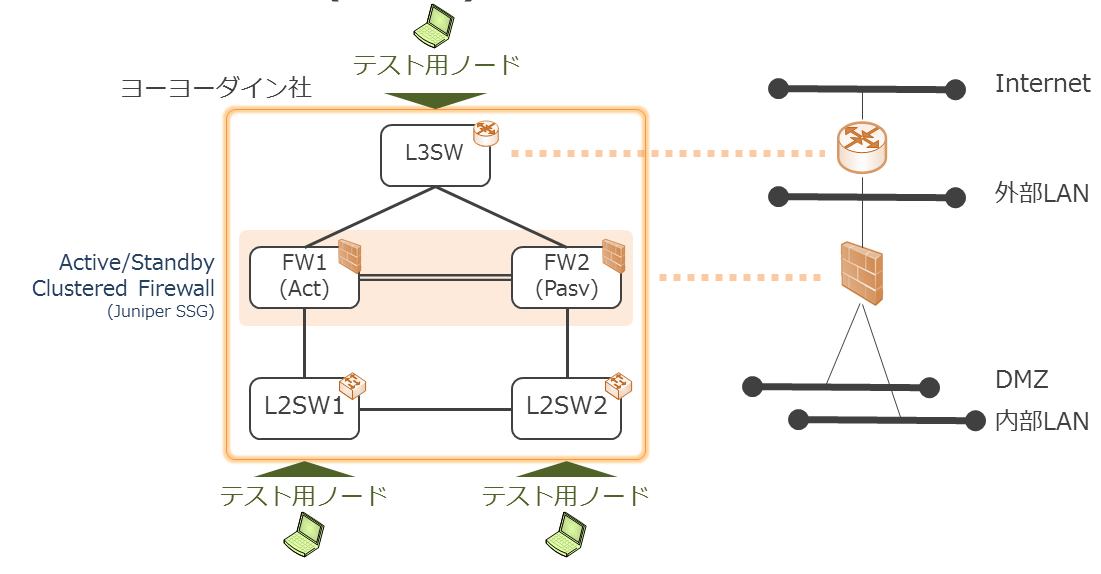
\includegraphics[scale=0.55]{img/poc-env-physical.png}
 \caption{PoC環境: 物理構成図(概要)}
 \label{fig:poc-env-physical}
\end{figure}

\begin{table}[h]
 \centering
 \caption{機器一覧}
 \label{tbl:device-list}
 \begin{tabular}[t]{l|l|l|l}
  \hline
  Host & Vendor & Device & Version \\
  \hline
  \hline
  FW1/2 & Juniper & SSG20 & ScreenOS 6.3.0r22.0 \\ \hline
  L3SW, L2SW1/2 & Cisco & Catalyst3750G-24TS & IOS 12.2(50)SE5 (ipservicesk9) \\ \hline
 \end{tabular}
\end{table}

% SSG, 当初使用していたのは 6.3.0r5.0

 \section{環境構成(管理系およびテストシステム)}
 \label{sec:mgmt-and-tester-nw}
 % - Tester Set について
 % - 構成図 \url{https://drive.google.com/open?id=0B2eRR_JxYJA5Nm1VbzBnR1FQMUk}
 % - Syslogについて

管理者要件(\ref{sec:logical-nw-design}節)のとおり、ネットワーク管理につ
いては \yo サービスネットワークと分離した構成をとる。
\figref{fig:poc-env-physical}のネットワーク機器(FW, L2/L3スイッチ)管理ア
クセスについては、次のように out-of-band な管理ネットワークを構成する
(\figref{fig:poc-env-physical-detail})。
\begin{itemize}
 \item Firewall: 管理用VRを設定し、管理用VRへ接続するインタフェースおよ
       びVLANをサービス用のものと分離する。
 \item L2/L3スイッチ: 管理用VRFを設定し、管理用VRFへ接続するインタフェー
       スおよびVLANをサービス用のものと分離する。
\end{itemize}

    \paragraph{Tester set}
\figref{fig:model-nettester}のように、NetTester server と対応する物理
OpenFlowスイッチのペアを、本プロジェクトでは「Tester Set」と呼ぶ。
NetTesterによるテスト作業は tester set の範囲内でおこなわれる。

PoCにあたって、検証環境(\figref{fig:poc-env-physical-detail})内ではふた
つのtester setを構築した。これは次の理由によるものである。
\begin{itemize}
 \item テストシナリオ実装のうち、並行して実装・テスト実行\footnote{テス
       トシナリオの動作テスト}が可能なものについて並行作業可能にするため。
 \item NetTesterのデバッグ、バグ再現調査などトラブルシュート対応のための
       切りわけ手段として。機器故障や環境依存のある問題を切りわけ、作業
       中断リスクを回避するため。
\end{itemize}

    \paragraph{Tester setによるテスト実装作業の制限}
テスト実行は原則としてひとつのtester setで実行されることを想定する
\footnote{ひとつのサーバ(OS)上で複数のNetTesterは実行できない。複数の
NetTester serverをまたいで排他制御をおこなう制御はNetTesterではなく外部
オーケストレータなどで実行する必要がある
(\ref{sec:testscenario-excl-ctrl}節)。}。並行作業や同時実行については以
下のような条件について考慮する必要がある。
\begin{itemize}
 \item テストシナリオ中で使用するテスト用ノード等のパラメタ重複: 例えば、
       同一IPのテスト用ノードを生成するテストシナリオを、ひとつのテスト
       対象ネットワーク内で同時に実行するような場合(デバッグや調査などで
       同一シナリオを異なるtester setで同時に実行するといったケース)。
 \item テスト実行中(実行前後)のテスト対象ネットワーク状態遷移: 例えば、
       リンク障害試験(「動的なふるまいのテスト」)では、操作対象となる物
       理リンクが1箇所となるためその物理リンクを制御可能なtester setはひ
       とつだけに限られる。
       \begin{itemize}
        \item 同様に、テスト実行中にトポロジなどが変化する想定をおいてい
              ない「静的なふるまいのテスト」も、「動的なふるまいのテスト」
              と同時に実行することはできない。
       \end{itemize}
\end{itemize}

\figref{fig:poc-env-physical-detail}ではtester set 1を「動的なふるまいの
テスト」用に使用するように設計している。テスト対象が物理ネットワークであ
り、ひとつのインスタンスからのみ操作可能なリソースがある点に注意が必要で
ある\footnote{NetTesterに外部から操作可能なAPIを実装して連携させるといっ
た応用も考えられるが、こうした応用は本プロジェクトの目標範囲外となる。}

    \paragraph{物理構成図補足}
\figref{fig:poc-env-physical-detail}にあるSSG5はFW(FW1/2)の設定や動作確
認用に使用したものである(OSはFW1/2と同様: \tabref{tbl:device-list})。
NetTester開発やテストシナリオ実装にあたって、FWの設定や挙動をテストシナ
リオ上から確認し、問題点の切りわけをおこなうために利用した。

\begin{landscape}
 \begin{figure}[h]
  \centering
  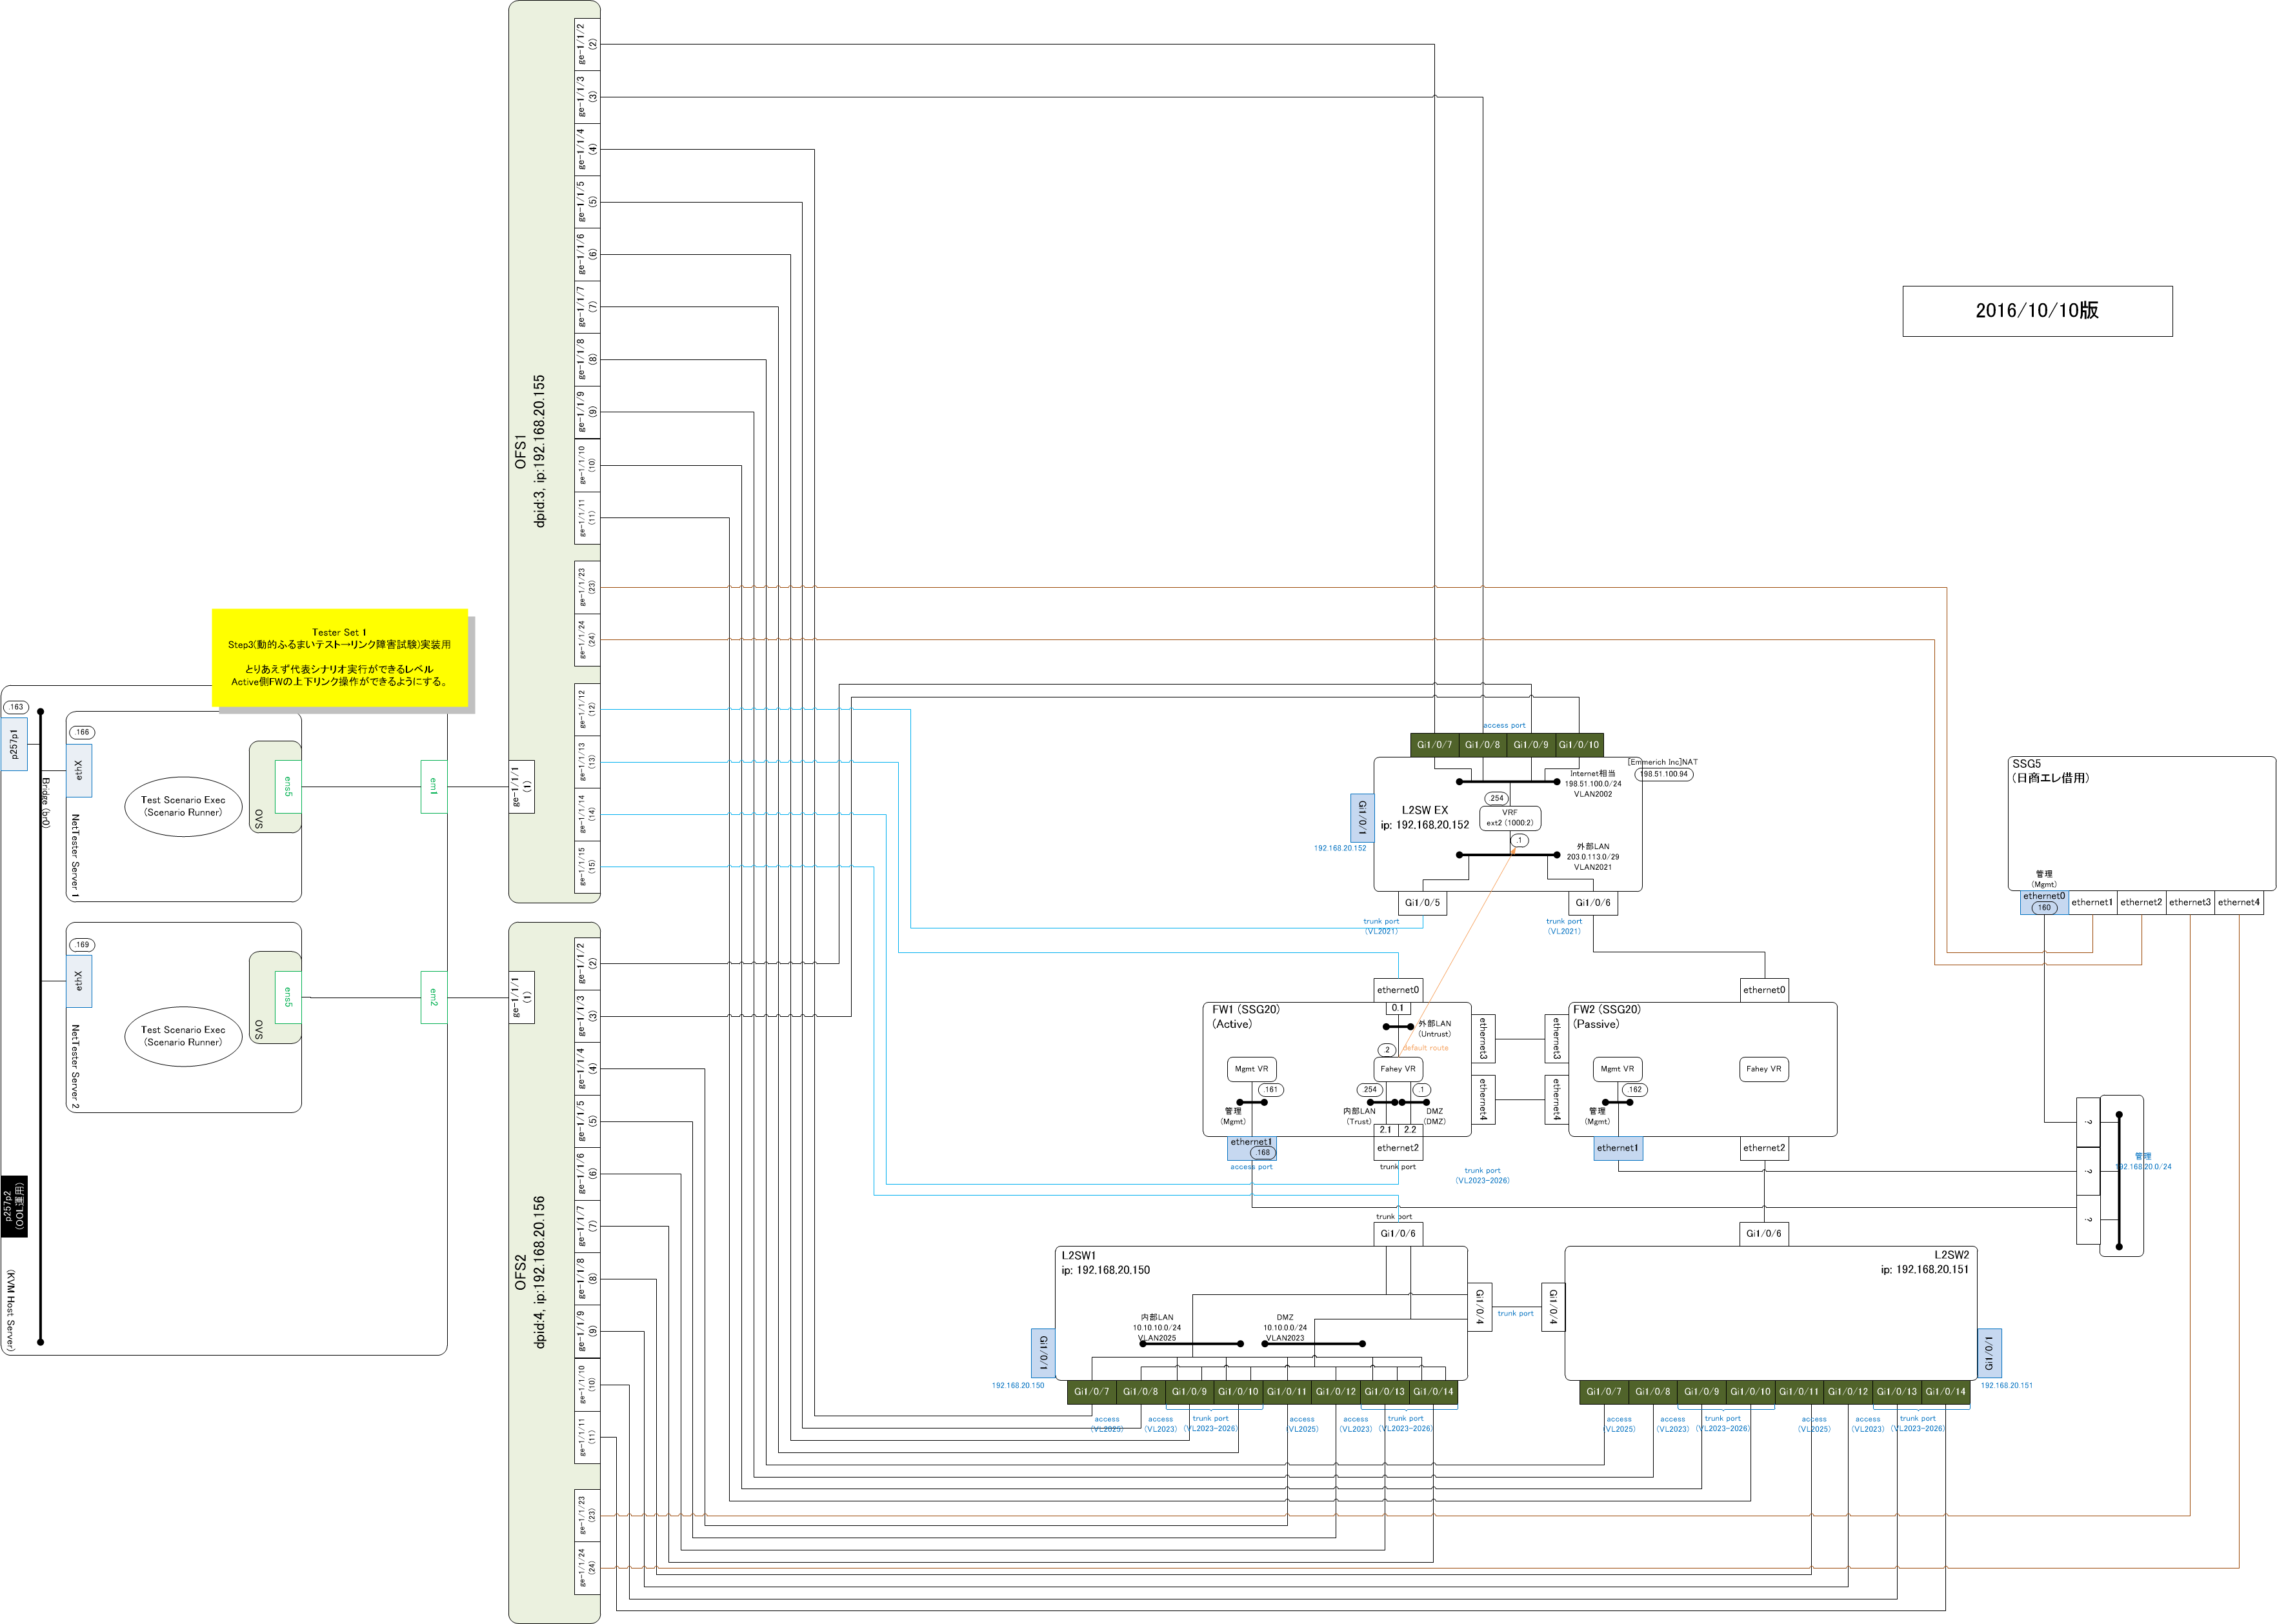
\includegraphics[scale=0.225]{img/poc-env-physical-detail.png}
  \caption{PoC環境: 物理構成図(詳細)}
  \label{fig:poc-env-physical-detail}
 \end{figure}
\end{landscape}


%%% Local Variables:
%%% mode: yatex
%%% TeX-master: "main.tex"
%%% End:

%% -*- coding: utf-8-unix -*-

\chapter{テストシナリオ実装}
\label{chap:poc-scenario-dev}

 \section{テストシナリオの概要}

  \subsection{ネットワークテストの方針}

\ref{chap:poc-target-design}章で設定したとおり、\yo ネットワークのテスト
を考える。そのためのテストシナリオとして「静的なふるまいのテスト」「動的
なふるまいのテスト」の2種類を実装する。テストシナリオ実装・テスト実行を
通して、物理ネットワークのテスト自動実行のポイント検討や問題点の抽出、従
来の人手によるテスト作業との比較を行なう。

  \subsection{BDDテストシナリオの基礎}
  % - TDD/BDDとBDDツールとしてのCucumber
  % - Narrative
  % - ネットワークテストを書く上での検討点、今回のプロジェクトでの方針・決めごと
  %   - なぜそうきめたのか?

      \paragraph{テストツール}
NetTesterはテスト用ノードの生成・テスト対象ネットワークへの配置(パッチ接
続)をおこなうためのAPIを提供する。提供されるAPIを使用して \yo ネットワー
クのテストを実装する。\footnote{実際に作成した自動テストのためのコードは
NetTester Examples~\cite{nettester-ex}として公開している。}

テストシナリオの記述については、アプリケーションのテストでつかわれる既存
のツールと連携することを想定している。本PoCでは、「BDDによるネットワーク
のテスト」を考えていること(\ref{sec:behavior-test}節)、広く使われている
ツールであること、RubyベースでNetTesterとの親和性が高いことをもとに、BDD
ツールであるCucumber\cite{cucumber}を採用した。

    \paragraph{Narrative}
    % Cucumber の .feature の書き方 – NetTester
    %   https://3.basecamp.com/3088280/buckets/867009/messages/155991347
    % クライアントの要望にこたえるWebサービス開発 ~「らせん型ワークフロー」のススメ~
    %  http://www.slideshare.net/mayuco/css-nite-in-sapporo-vol5-14085124
BDDでは、テストのストーリー(フィーチャ)を以下のような構造で記述する
\cite{rspec-book,spiral-workflow}。
\begin{description}
 \item[タイトル] どのストーリーについて説明するのかを示す。タイトルは一
            般に、ユーザがシステムに要求するかもしれないアクティビティを
            短い言葉で表したものになる。
 \item[ナラティブ] ストーリーの内容について説明をする。一般的には
            Connextraフォーマットと呼ばれる形式の短い文章で記述される。
            このテンプレートは、誰がシステムを使っていて、そのユーザは何
            をしていて、なぜそのことに関心があるのか、を明確にする。
            \begin{itemize}
             \item ``As a (role)'': [誰のために(role)]として
             \item ``I want (feature)'': [何を(feature)]したい
             \item ``So that (bussiness value)'': なぜなら[なぜ
                   (bussiness value)]のためだ
            \end{itemize}
 \item[受け入れ基準] ストーリーの完了・完成を定義する受け入れ基準、シナ
            リオの定義。
\end{description}

Cucumberにおけるフィーチャとは、システムを利用するユーザーまたは別のコン
ピュータの視点に立っておおまかに表現された要件のことを指す。Cucumberの
フィーチャはタイトルと簡単なナラティブ、受け入れ基準としての役割をはたす
自動化されたシナリオによって構成される。
\begin{itemize}
 \item フィーチャはタイトルとナラティブで構成され複数のシナリオを含む。
       (本プロジェクトでは\verb|features/*.feature|ファイル)
       \begin{itemize}
        \item シナリオはそれぞれ、シナリオ内でおこることを任意のステップ
              で記述する。
       \end{itemize}
 \item 個々のステップ定義は開発で使っているシステムの言語で記述される。
       (本プロジェクトではRuby: \verb|features/step_definitions/*.rb|ファ
       イル)
\end{itemize}

% Narrative を Pull Requst する – NetTester
%   https://3.basecamp.com/3088280/buckets/867009/todos/159223633
% NetTester機能拡張(NW機器間接続)方針・やりたいこと – NetTester
%   https://3.basecamp.com/3088280/buckets/867009/todos/182746431
% Firewall の cucumber シナリオ – NetTester
%   https://3.basecamp.com/3088280/buckets/867009/todos/158299550

 \section{静的なふるまいのテストの実装}
% テストシナリオ策定の考えかた…そもそもなにをするテストなのか。どのような
% 検討を経てテストシナリオをきめたのか。narrativeの定義のプロセスとか。
% TODO: OOD資料にかいたようなテストコード解説のはなしをこちらにも含めるか?
% - 実装
%   - Step2テスト業務で気づいたことをまとめる – NetTester
%     \url{https://3.basecamp.com/3088280/buckets/867009/todos/260220903}

  \subsection{テストとして実現したいこと}
ネットワークに対して最低限要求されることは、ネットワークを介して必要な通
信が実現できることである。ネットワークの目的は、大きく言えばコミュニケー
ションを実現することである。あるノードが、他のノードと、必要な手段(アプ
リケーション)で通信できるかどうか、という点がまず初めにネットワークに求
められる機能要求となる。

「ネットワークの静的なふるまい」(\ref{sec:behavior-to-test}参照)では、ネッ
トワークが定常状態にある(一定の状態にあって状態変化しない)ときに、ネット
ワーク利用者が実現したいend-to-endの通信がすべて実現可能かどうかをテスト
する。

  \subsection{テスターに求められる機能}

テストで確認したいend-to-endの通信、すなわち、実現したい通信要求は、通信
をおこなうノード(エンドポイント)の論理的・物理的な配置の組合せに応じて異
なる。また、通信をおこなうアプリケーションによっても別途制御がおこなわれ
る。例えば、LBやDPI\footnote{Deep Packet Inspection}をおこなうFWなどがネッ
トワーク内にある場合は、単純な宛先(ヘッダ)情報だけではなく、やりとりされ
るアプリケーションレベルの情報によって通信の可否などが変化する。

したがって、単純なend-to-endの通信試験だとしても、配置やアプリケーション
の組合せによって大量のテストケースが発生してしまう、テストのためのリソー
ス確保などが充分にできない、などの課題があった
(\ref{sec:discuss-network-test}参照)。

そこで、テスター(NetTester)では以下の機能が要求される。
\begin{itemize}
 \item テスト用ノードの生成
 \item テスト用ノードの配置
 \item テスト用ノード上でのタスク実行
 \item 複数のテスト用ノード操作/集中管理
\end{itemize}
NetTesterはこうしたノードの生成・配置・集中制御の機能(API)を提供している。
テストシナリオ(Cucumber)ではBDDの考えかたに基づいて、ノード間でどういっ
た通信を実現する必要があるかを個別の通信要件
(\tabref{tab:poc-requires-yo-int},\tabref{tab:poc-requires-yo-dmz},\tabref{tab:poc-requires-etc})
ごとに定義する。

 \section{動的なふるまいのテストの実装}
% 障害試験シナリオを書く – NetTester
% \url{https://3.basecamp.com/3088280/buckets/867009/todos/238169066}
% Step2to3タスク検討
% https://drive.google.com/open?id=0B2eRR_JxYJA5M1RGdEZaOFkxTFk

  \subsection{テストとして実現したいこと}
% NetTester機能拡張検討
% https://drive.google.com/file/d/0B2eRR_JxYJA5TmhaeWItNF93Um8/view
ネットワークは状況に応じて状態を変化させる。変化のトリガとして、例えば障
害発生による冗長経路への切替、メンテナンスのための一部のデバイスの停止や
切り離し・そのための通信経路迂回、ネットワーク機器の追加(拡張)や削除(縮
小)などがある。こうしたイベントに対して、ネットワーク(全体)は、ネットワー
クの状態と発生したイベントに応じて自らの情報(状態)を自律的に更新し、トラ
フィックの経路を変更するなどの制御をおこなう。

「ネットワークの動的なふるまい」(\ref{sec:behavior-to-test}参照)では、ネッ
トワークが状態変化するときに、ネットワーク利用者へ与える影響が許容範囲内
かどうかをテストする。ネットワーク利用者への影響とは、ネットワーク状態遷
移中に発生するトラフィックの継続可否、影響度・影響範囲(場所的な範囲や時
間)である。例を以下にあげる。
\begin{itemize}
 \item トラフィックの継続可否
       \begin{itemize}
        \item ロードバランサなどL7の情報にしたがってトラフィックを操作す
              るような機器では、冗長系切替のときに、セッション情報などを
              引きついでアプリケーション通信を維持することが求められる。
              同様にNATなどの変換テーブルに基づいてトラフィックを操作す
              る機器でも冗長系機器間で状態の同期が必要になる。
        \item 系切替には隣接する機器も関連する。例えば、対象とする冗長系
              のL1/L2の切替に Gratuitous ARP を使用する機器で、隣接する
              L2スイッチのバグによって Gratuitous ARP 処理が正しくおこな
              われず、全体としてトラフィックの継続に失敗した事例などがあ
              る。
       \end{itemize}
 \item 影響度・影響範囲
       \begin{itemize}
        \item 状態変化によって予期しない現象が予期しない範囲でおこること
              がある。範囲としては、物理的な場所(特定のスイッチの配下な
              ど)・論理的な場所(特定のL2セグメントなど)複数の要素が考え
              られる。
        \item 仮想化によって物理構成と論理構成は分離されることが一般的で
              ある。この際、物理構成操作のオペミスや論理構成操作のミス
              (記述ミスや勘違い)によったわずかなミスの見落としがセグメン
              ト全体をまきこむL2ループを引き起すことがある。
        \item 機器のバグや設定ミス、そのほかの機能との併用による機器CPU
              専有状況の発生などがあると、こうした系切替によるトラフィッ
              クの維持・継続ができなかったり、想定した時間内に完了できな
              いことがある。例として、多数のVLANを収容していたL3スイッチ
              で、系切替の際のSTPトポロジ再計算処理によるCPU専有が発生し、
              スイッチ配下のセグメント全域で広範囲にわたって切替時間の遅
              延・それにともなうトラフィックの維持失敗(タイムアウト発生)
              がおこってしまった事例などがある。
       \end{itemize}
\end{itemize}

いくつか例を挙げたが、これらの問題はネットワーク全体(系全体)の相互作用に
影響される。ネットワークの場合はベンダや機器ごとに独自のOSやアーキテクチャ
を持つものが多く、特定機能や製品を組み合わせたときの相性問題やキャパシティ
問題、特定ハードウェアやソフトウェア(バージョン)のトラブルといった情報を
共有することは難しい。また、複数の冗長化機能(複数の機器にまたがるものも
含む)の連動する際、状態遷移のタイミングなどで機能単体では問題なく動作す
る機能が複合した結果、問題が発生することもある\footnote{例として:
OSPF/BGP収束時間差によるブラックホールやループの発生
\cite{j3g14-packet-forwarding}など。}。こうした理由により、ネットワーク
の操作・状態変化において、すべての影響を予想するのは非常に困難である。

動的なふるまいのテストでは、上に挙げた「トラフィックの継続可否」「影響度・
影響範囲」のテストを自動化することを目標とする。

  \subsection{テスターに求められる機能}
  % 求められる機能、今回実装したもの

「動的なふるまいのテスト」では、次のような機能が必要となる。
\begin{description}
 \item[イベントの生成] ネットワークの状態変化を発生させるためのイベント
            を発生させる機能。今回のPoCではリンク障害試験をターゲットと
            するので、何らかの形でリンク障害を発生させる必要がある。
 \item[イベント発生時のトラフィック影響調査] ネットワークが状態変化する
            タイミングで、ネットワーク上のトラフィックがどの程度の影響を
            うけているかを調査する必要がある。
\end{description}

一般的には、ネットワークの状態変化イベントによって影響をうけることが予想
されるトラフィックをあらかじめ生成しておき、イベント発生・ネットワーク状
態変化の収束をまって、トラフィックに最終的にどのような影響があったのかを
調査する。したがって、複数のノード間において・同時並行で・トラフィックを
継続生成(送受信)しながらイベントを発生させる機能が必要となる。

  \subsection{システム構成}
PoC環境(詳細は\figref{fig:poc-env-physical-detail})では
\figref{fig:poc-env-linkdown}のようにtester set 1を「動的なふるまいのテ
スト」用に使用するよう設計している。PoCでは、\yo 内部ネットワークの中心
となるFWの冗長化機能試験をおこなう。そのため、テストシナリオではFWの
Active/Passive切替トリガとなるActive側(FW1)リンクダウン/リンクアップ操作
を実装する。物理リンク操作のため物理OpenFlowスイッチ(OFS1)へ以下の2リン
クをそれぞれ引き込んでいる。
\begin{itemize}
 \item L3SW-FW1 間リンク (FW1 Uplink)
 \item FW1-L2SW1 間リンク (FW1 Downlink)
\end{itemize}

\begin{figure}[h]
 \centering
 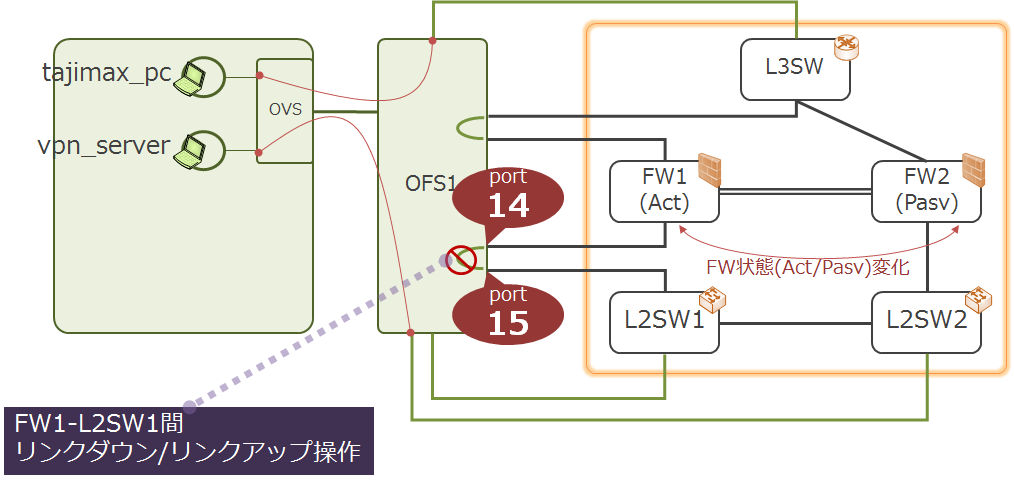
\includegraphics[scale=0.6]{img/poc-env-linkdown.png}
 \caption{PoC環境: NetTesterによるリンクダウン操作}
 \label{fig:poc-env-linkdown}
\end{figure}

 \section{テストシナリオ実装における検討ポイント}

  \subsection{Teardown処理}

CI/CDといったプロセスを実現する上で、複数・任意のテストシナリオをまとめ
て実行することが求められる(回帰テスト含む)。

テストシナリオはいずれも、テスト対象が所定の初期状態にあるところから実行
を開始しなければ狙った「ふるまい」を調査することができない。ソフトウェア
の自動テストでは、テスト対象となるアプリケーション(プロセス)やインスタン
スは初期状態で起動しなおすことが容易なため、常にアプリケーションやインス
タンスを起動しなおして初期状態からのテストをおこなうのが一般的である。

しかし、ネットワーク(特に物理ネットワーク)を対象としている場合はテスト対
象が物理的に存在している。よって、そのままでは、前のテストシナリオ実行直
後のネットワーク状態が次のテストシナリオ実行開始時の初期状態となってしま
う。個々のテストシナリオ実行のたびにネットワーク(機器)の初期化・再構築す
ることは、不可能ではないが以下の理由により難しい。
\begin{itemize}
 \item 機器によっては、コンフィグ消去・再起動に数分から十数分かかるもの
       がある。
 \item 再起動によるteardown処理をおこなう場合、ネットワーク機器の起動順
       序によりネットワーク全体の状態が変化し得る。
 \item コンフィグリセット操作に失敗すると再起動後にリモートアクセスでき
       ず、復旧作業(現地作業)が必要になるリスクがある。
\end{itemize}
特に本PoCでは、静的なふるまいのテストとして数十の通信要件をテストするた
めのシナリオを連続実行したいという要求があるため、単一テストシナリオ実行
の時間的なオーバーヘッドが大きいことが問題となる。

そのため、テストに応じて何らかの形でネットワークの状態を初期状態に戻すた
めの処理(teardown処理)を実装する必要がある。本PoCではL2-L4の状態に着目し
て、以下のteardown操作を実装している。

    \paragraph{Target network の状態操作}
テスト対象ネットワーク各機器のL2-L4の状態をクリアする(CLIによる各種
\code{clear}コマンドの実行)。
\begin{itemize}
 \item MACアドレステーブル/ARPキャッシュのクリア
 \item FWの NAT Table のクリア
 \item FWの active/standby 状態のクリア
       \begin{itemize}
        \item 今回、動的なふるまいのテストにあたって、FWは障害が発生した
              リンクの復旧にあわせて active/passive を自動復旧するように
              設計したため、特に操作していない
              (\ref{sec:physical_nw_design}参照)。
       \end{itemize}
\end{itemize}

    \paragraph{Netns の /etc 配下のSetup/Teardown}
    % 自作echoサーバーで通信開始時に10秒のラグが起きる問題 – NetTester
    % https://3.basecamp.com/3088280/buckets/867009/todos/274457003

NetTesterでは、Network namespace でテスト用ホストを生成する。このときバッ
クエンドでは iproute2(\code{ip}コマンド)を使用している。iproute2 によっ
て生成されたホスト(netns)では、\verb|/etc/netns/<netns>/| が etc ディレ
クトリとしてマウントされる~\cite{iproute2-doc}。そのため、テスト用ホスト
内部での名前解決などでは、実体としては \verb|/etc/netns/<netns>/hosts|,
\verb|resolv.conf| を参照する。これらの設定ファイル等が正しく設定されて
いないと名前解決がタイムアウトするなどの問題が発生する。

    \paragraph{物理OFSのflow tableのクリア}
物理OpenFlowスイッチには、テストのたびにフローエントリが登録される。その
ため、テストの実行のたびにフローエントリのクリア処理が必要となる。

本PoCでは、テスト用ホストのMACはテスト実行時にランダムに設定するよう実装
したため、テスト実行をくりかえすと多数の不要なフローエントリが物理スイッ
チ上に残る。テスト用ホストのMACアドレスを固定にすることでフローテーブル
の消費は抑えられるが、異なる用途で同一のMACアドレスを使いまわすなどのケー
スで、予期しない動作不具合が発生するおそれがある\footnote{NetTesterのテー
ブル設計では、テスト用ホストのMACアドレスをキーとして、フロー優先度
(priority)による制御をおこなう(\ref{sec:flow-priority-design}参照)。同一
MACアドレスを異なる用途で使いまわす場合、他の用途として設定したフローエ
ントリとマッチしてしまい、狙ったパッチ動作が実現できない恐れがある。}点
に注意すること。

\section{並列実行と排他制御}

物理ネットワークをテストする場合、テスト対象(物理ネットワーク)は原則ひと
つしかない。テストの数が多くなる場合、複数のテストを同時に実行することが
考えられるが、現状NetTesterを使ったテスト自動化は並行実行は原則としてで
きない。以下にその理由を列挙する。

\begin{description}
 \item[状態操作の競合] テストシナリオごとに、想定しているテスト対象ネッ
            トワークの状態がある。それらを変化させるテストシナリオは同時
            に実行できない。
            \begin{itemize}
             \item テストシナリオAを実行している途中で、テストシナリオB
                   がteardown処理を実行して、テスト対象ネットワークの状
                   態クリアをしてしまうと、テストシナリオAで想定していた
                   状態を変化させてしまう\footnote{Teardown処理として
                   \code{clear}コマンドを使用しているが、特定シナリオで
                   使うエントリだけを消去するのではなく、NW機器全体の情
                   報をまとめて消去してしまうため。そのシナリオに依存す
                   るエントリだけをねらって消去できるのであればこの制約
                   は外れるが、テスト対象ネットワーク内の機器それぞれに
                   ついて対応可能かどうかという点が問題となるだろ
                   う。}\footnote{あるいは、teardown処理を他のテストシナ
                   リオ実行がおわるまで待機し、まとめて実行できればよい
                   が、現状はそうした実装をおこなっていない。}。
             \item 動的なふるまいのテストのように、ネットワーク全体の状
                   態に影響をあたえるようなテストシナリオは同時に実行で
                   きない。
            \end{itemize}
 \item[ネットワークリソースの競合] テスト対象ネットワークで一意でなけれ
            ばならないリソースの操作については同時に実行できない。
            \begin{itemize}
             \item テストシナリオA/Bが同じIP/MACを持つテスト用ホストを同
                   時に生成してしまうと、テスト対象ネットワーク内で
                   IP/MACの重複が発生してしまう。
             \item 物理リンクの操作など、ひとつしか存在しないリソースの
                   制御が必要なテストシナリオは同時に実行できない。
            \end{itemize}
\end{description}

本PoCでは\figref{fig:poc-env-physical-detail}のようにふたつのtester set
を使用しているが、これはあくまでもデバッグ用途のためである。Tester set
を複数用意することで、静的なふるまいのテスト(NWが定常状態にある)で、かつ
同じIP/MACのテスト用ノードを使用せず、teardown 処理をテストシナリオ単位
で実行しないようなケースに限って複数のテストが実行可能となる。

上記の制約の一部については、NetTesterで実行されるタスクの排他制御のしく
みを導入することで対応できるものがあるが、現状はそうした対応については本
PoCの範囲外としている。本PoCでは、ひとつのテスト対象ネットワークに対して
tester setがあり、同時にひとつのテストシナリオを実行することが前提となっ
ている。

\subsection{テストシナリオのサイズ}

シナリオサイズの目安、シナリオ分割の目安 (step3 test つくっているときに
分割するって話になった理由は?)

\subsection{ステップ実装上の工夫}
\begin{itemize}
 \item ニセ○○サーバとステップ実装 – NetTester \url{https://3.basecamp.com/3088280/buckets/867009/documents/216490375}
 \item コマンドをバックグラウンド実行 – NetTester \url{https://3.basecamp.com/3088280/buckets/867009/documents/216399643}
 \item step内でのバックグラウンドコマンド実行 – NetTester \url{https://3.basecamp.com/3088280/buckets/867009/todos/202691188}
 \item factory\_girl で仮想ホストを作る – NetTester \url{https://3.basecamp.com/3088280/buckets/867009/documents/210831650}
\end{itemize}

\section{PoCの結果と評価}

\subsection{実際に発見できた問題点}
テストとしての結果まとめ
\begin{itemize}
  \item 結果: 実際に発見できたトラブルや設定ミスなどをあげる。
       \begin{itemize}
        \item Teardown関連
              \begin{itemize}
               \item 原因切り分けメモ (muraki) – NetTester \url{https://3.basecamp.com/3088280/buckets/867009/documents/217782147}
               \item 調査: テスト環境でシナリオ実行すると2回目以降でコケる – NetTester \url{https://3.basecamp.com/3088280/buckets/867009/todos/218486066}
              \end{itemize}
        \item Target Network の設定不備の発見
              \begin{itemize}
               \item DNSのテスト作る – NetTester \url{https://3.basecamp.com/3088280/buckets/867009/todos/301325453}
               \item 通信要件\#10 A社内PC→インターネットの疎通確認(ICMP) – NetTester \url{https://3.basecamp.com/3088280/buckets/867009/todos/233175867}
               \item 通信要件\#29 B社PC→DMZ内のVPNサーバの疎通確認(SSLVPN) – NetTester \url{https://3.basecamp.com/3088280/buckets/867009/todos/233178490}
              \end{itemize}
       \end{itemize}
\end{itemize}

step3
\begin{itemize}
 \item 実装 (NAT IPの変更とかデモの話をどこまで含めるか?)
 \item 結果
\end{itemize}

\subsection{ネットワークの構築・運用プロセスに対する定性的な評価}
評価・考察
\begin{itemize}
 \item 体制や役割分担/タスクとスキルセットについて: ref.\url{https://3.basecamp.com/3088280/buckets/867009/todos/260220903}
 \item テスト実装のコスト
 \item 繰り返し実行できることのメリット
       \begin{itemize}
        \item OSの更新などおおきな変更にたいするリスクヘッジ
       \end{itemize}
\end{itemize}


%%% Local Variables:
%%% mode: yatex
%%% TeX-master: "main.tex"
%%% End:

%% -*- coding: utf-8-unix -*-

\chapter{おわりに}

 \section{まとめ}
 \label{sec:summary}

複数の機器や技術の整合性をとらなければいけないネットワークは、複雑になり
がちで設定変更や障害の影響範囲を予測しにくい。しかしサービス提供者は、利
用者の要求変化に応じて、安定した通信サービスを迅速かつ柔軟に提供していく
ことが求められる。そのためには、検討可能範囲や許容されるリードタイムに限
界がある人によるレビューではなく、ネットワークが機械的・自動的にテストで
きること、テストによってネットワークが設計通りの機能を提供していることを
確認できることが重要となる(\ref{chap:problem-setting}章)。本プロジェクト
では特に、ネットワークの「ふるまい」に注目して(\ref{chap:approach}章)、
物理ネットワークの自動テストをおこなうシステムを開発し
(\ref{chap:nettester-design}章・\ref{chap:nettester-usage}章)、いくつか
のユースケースについて実際にシナリオテストの実装をおこなった
(\ref{chap:poc-target-design}章・\ref{chap:poc-scenario-dev}章)。

テストシナリオ実装においては、ネットワークが定常状態に状況でのend-to-end
通信を「静的なふるまいのテスト」、リンク障害による通信経路切替がおきてネッ
トワークの状態が変化する状況でのend-to-end通信を「動的なふるまいのテスト」
とした。これらのテスト実装によって、定常状態でのアプリケーションレベルで
の通信試験だけでなく、障害試験のように物理構成操作が必要で従来は人手で作
業しなければいけなかった試験についても自動化ができるようになった。本書で
はこれらの物理ネットワーク試験自動化における実装例と実装の際に発生した課
題に対する対処などについて解説している。

本プロジェクトで実証したユースケースは単純化したものになっているが、物理
ネットワークでおこなうテストとして通常実施される、基本的な作業を自動化し
たものである。本プロジェクトで整備した「ふるまい」レベルでのネットワーク
テスト機能により、\ref{sec:discuss-network-test}節で示したネットワークテ
スト自動化のための基本機能は一通りそろえることができたと考える。

 \section{今後の課題}
 \label{sec:future-work}
 % - 今後想定される運用・開発のプロセス
 % - 「できないこと」のテスト
 % - 実用トライアル

現時点では、架空の企業ネットワークを想定した小規模かつシンプルなネットワー
クでのPoCを行なっている。しかし、実際に実環境・実運用で使用する場合は、
より複雑な環境・要件に対応していくことが求められる。

\ref{sec:summary}節で示したように、ネットワークテストの基本機能はおおむ
ね整備できた。今後は実環境での利用を想定した実用トライアルにむけた活動を
進めていく。そのなかで、\ref{sec:desired-and-target}節で示したようなネッ
トワークにおけるCI/CDプロセスの確立、そのためのツールチェーンのありかた
や実装などについての検討をおこなう。また、開発したツールについて、実際の
問題解決のために必要な機能・非機能面での機能強化を進める。


%%% Local Variables:
%%% mode: yatex
%%% TeX-master: "main.tex"
%%% End:


\appendix
%% -*- coding: utf-8-unix -*-

\chapter{用語}
\label{cpt:termdef}

表\ref{tbl:termdef} に本書で使用している用語・略語の一覧を示す。一般的な
用語については特に解説をくわえない。

 \begin{longtable}{p{8em}|p{8em}|c|c|p{16em}}
  \caption{用語定義}
  \label{tbl:termdef}
  \\
  \hline
  用語 & 英語表記 & 略語 & 分類 & 意味\\ \hline
  \hline
  \endhead
  沖縄オープンラボ & Okinawa Open Laboratory & OOL & 一般 & (略語定義) 一般社団法人 沖縄オープンラボラトリ \url{https://www.okinawaopenlabs.org/} \\ \hline
  ネットワーク & Network & NW & 一般 & (略語定義) \\ \hline
  ファイアウォール & Firewall & FW & 一般 & (略語定義) \\ \hline
  ロードバランサ & Load Balancer & LB & 一般 & (略語定義) \\ \hline
  & Virtual Private Network & VPN & 一般 & (略語定義) \\ \hline
  L1パッチ & L1patch & & プロジェクト & 一般的なネットワーク用パッチパネル(物理結線を集中して付け替えるための機構)。本書では「ネットワーク用パッチパネルと同等のことをおこなえるシステム」として使う。 \\ \hline
  & OpenFlow & OF & 一般 & (略語定義) \\ \hline
  & OpenFlow Switch & OFS & 一般 & (略語定義) \\ \hline
  & OpenFlow Controller & OFC & 一般 & (略語定義) \\ \hline
  テスト対象ネットワーク & Target/Testee Network & & 一般 & 動作確認を行いたいネットワーク。複数のネットワーク機器から構成される。\\ \hline
  テスター & Tester & & プロジェクト & 本書で単に「テスター」とした場合はネットワークテスター(ネットワークテストシステム): NetTester のことを指す。\\ \hline
  テスト対象機器 & Device Under Test & DUT & 一般 & テスト対象となる個々の機器。テスト対象ネットワークを構成するいずれかひとつの機器。\\ \hline
  & Open vSwitch & OVS & 一般 & Linux上で動作するL2スイッチ/OFS実装。 \\ \hline
  & NetTester & & プロジェクト & 本プロジェクトで開発したネットワークテストツール。 \\ \hline
  & Cucumber & & 一般 & BDDテストツール/テストシナリオ記述言語。 \\ \hline
  継続的インテグレーション & Continuous Integration & CI & 一般 & (略語定義) \\ \hline
  継続的デリバリ & Continuous Delivery & CD & 一般 & (略語定義) \\ \hline
  ふるまい駆動開発 & Behavior Driven Development & BDD & 一般 & (略語定義) \\ \hline
  テスト駆動開発 & Test Driven Devleopment & TDD & 一般 & (略語定義) \\ \hline
 \end{longtable}

%%% Local Variables:
%%% mode: yatex
%%% TeX-master: main.tex
%%% End:

%% -*- coding: utf-8-unix -*-

\chapter{関連ソフトウェア}

 \section{Expectacle}
 \label{sec:expectacle}
 % tftp server – NetTester
 % \url{https://3.basecamp.com/3088280/buckets/867009/documents/268762822}
 % GitHub - stereocat/expectacle
 % \url{https://github.com/stereocat/expectacle/tree/develop}

テストシナリオ実装の際、テスト対象機器へのコマンド発行(teardown処理;
\ref{sec:teardown}節)をおこなうためにExpectacle~\cite{expectacle}という
ツールを使用している。Expectacle はあらかじめ作成したコマンド(列)を指定
した機器情報に基づいて順に送信する単純なツールである。詳細な使用方法につ
いてはExpectacle README にあるためここでは扱わない。本PoCで利用した際の
注意事項について解説する。

Expectacle は、操作対象となる機器と機器に送信するコマンド列の情報を使用
するが、その中ではERBを使った変数の展開ができる。本PoCでは、機器情報のう
ち、そのまま設定ファイルに記入してリポジトリへ登録してはいけない秘密情報
(ログインユーザ名・パスワード)を設定するために環境変数を使用した。例とし
て、L2/L3スイッチの操作に関する機器情報は
\lstref{lst:l2sw1-login}\footnote{\url{https://github.com/net-tester/examples/blob/feature/ood_demo/features/support/expectacle/hosts/c3750g_hosts.yml}}
のようになる。
\begin{lstlisting}[caption=L2スイッチ(L2SW1)ログイン情報,label=lst:l2sw1-login]
- :hostname : 'l2sw1'
  :type : 'c3750g'
  :ipaddr : '192.168.20.150'
  :protocol : 'ssh'
  :username : "<%= ENV['L2SW_USER'] %>"
  :password : "<%= ENV['L2SW_PASS'] %>"
  :enable : "<%= ENV['L2SW_PASS'] %>"
\end{lstlisting}
\lstref{lst:l2sw1-login}ではログインユーザ名(\verb|L2SW_USER|)とパスワー
ド(\verb|L2SW_PASS|, ログイン/イネーブルが同一パスワード)を環境変数を参
照して設定している。そのため、テストシナリオ実行前に
\lstref{lst:l2sw1-login-envvar}のように環境変数を定義しておく。
\begin{lstlisting}[language=sh,caption=ログイン情報環境変数の設定,label=lst:l2sw1-login-envvar]
export L2SW_USER=username
export L2SW_PASS=password
\end{lstlisting}

環境変数によるパスワード等の設定は、そのままではコマンドヒストリ等に残っ
てしまうことがあるため、実行方法に注意が必要である\footnote{Expectacleで
は標準入力から環境変数の値を設定するスクリプトを同梱している:
\url{https://github.com/stereocat/expectacle/blob/develop/exe/readne}}。
Expectacleの機能は\tabref{tab:test-functions}の No.1 (NW機器の設定・操作)に
相当する。この機能は本プロジェクトの主要なスコープとしていないため、この
ような簡易な方法を採用している。

 \section{Debugging Trema}
 \label{sec:debugging-trema}
% 謎PacketInで死なずにログを出す – NetTester
% \url{https://3.basecamp.com/3088280/buckets/867009/todos/221324759}
% - Tremaのエラーログを出す – NetTester
%   \url{https://3.basecamp.com/3088280/buckets/867009/todos/210777914}
% - 今日なにした? – NetTester
%   \url{https://3.basecamp.com/3088280/buckets/867009/questions/181826801/answers/2016-09-08#__recording_221236017}

本プロジェクトの実行にあたって発生したOpenFlow関連の問題についての対処方
法(Tips)をまとめる。

  \subsection{Trema.logger}
  \label{sec:trema-logger}

当初、NetTester OFCのテーブルミスアクションを\code{CONTROLLER}として
packet-inを発生させるようにしていた。このとき、特定パケット(フレーム)の
packet-inに対して OFC (Trema) がエラーで停止しまうという問題が発生した
(\ref{sec:flow-priority-design}節)。この問題にあたって、Trema開発チーム
の協力により、Tremaの内部ログを取得するための、\code{Trema.logger} APIが
追加されている~\cite{trema-logger-doc}。

\code{Trema.logger}の使用方法は一般的なロガーと同様であり、Trema内部にロ
グメッセージを挿入していくことで、Trema内部のログを取得できる。たとえば
使用例は\lstref{lst:trema-logger-example}のようになる。
\begin{lstlisting}[caption=\code{Trema.logger}使用例,label=lst:trema-logger-example]
# lib/trema/switch.rb
def expect_receiving(expected_message_klass)
  loop do
    message = read
    # コントローラが受け取った OpenFlow メッセージをデバッグプリント
    Trema.logger.debug "Received an OpenFlow message: #{message.inspect}"
\end{lstlisting}

出力先のログファイルは \code{[ログディレクトリ]/trema.log} とな
る。\code{Trema.logger}を実行し内部ログを取得する場合、次のように実行時
ログレベルを指定する必要がある。
\begin{lstlisting}
trema run -l debug <controller>.rb
\end{lstlisting}
または verbose オプションを指定する(ログレベルは debug になる)。
\begin{lstlisting}
trema -v run <controller>.rb
\end{lstlisting}

  \subsection{Packet-in Binary Analysis}
  \label{sec:trema-packet-in-analysis}

\ref{sec:trema-logger}節の事例(特定packet-inによるOFCの停止)については、
実際にpacket-inするバイナリを解析し、原因がTrema/Pio~\cite{pio}パケット
パーサのバグであることを突き止めた。ここではその際のデバッグ方法を記載す
る。

    \paragraph{OFCパケットキャプチャ}
Tremaがどのようなタイミング・原因で停止するのかを調査するため、OFS-OFC間
のOpenFlowメッセージをパケットキャプチャし、OFC停止タイミングとの突合せ
をおこなった。これによって、あるパケット(フレーム)がpacket-inするタイミ
ングで、OFCの停止がおきるという仮説をたてた。

    \paragraph{\code{Trema.logger}によるpacket-inのダンプ}
Tremaの内部状態を取得するために、\code{Trema.logger}を追加して、コントロー
ラ停止時に処理していたpacket-inのダンプを取得する
(\lstref{lst:packet-in-dump})。
\begin{lstlisting}[language=,caption=問題となるPacket-inの取得,label=lst:packet-in-dump]
diff --git a/lib/trema/switch.rb b/lib/trema/switch.rb
index 5a73005..d8c222e 100644
--- a/lib/trema/switch.rb
+++ b/lib/trema/switch.rb
@@ -34,7 +34,9 @@ module Trema
     end

     def read
-      OpenFlow.read read_openflow_binary
+      openflow_binary = read_openflow_binary
+      Trema.logger.debug openflow_binary.unpack('C*').inspect
+      OpenFlow.read openflow_binary
     end

     private
\end{lstlisting}

これにより、\lstref{lst:packet-in-log}のようにpacket-inダンプが取得できた。
\begin{lstlisting}[language=,caption=得られたPacket-in dump,label=lst:packet-in-log]
 D, [2016-09-14T11:29:41.312256 #21392] DEBUG -- : [1, 10, 0, 146, 0, 0, 0, 0, 0, 0, 1, 24, 1, 216, 0, 4, 0, 0, 1, 0, 12, 204, 204, 204, 0, 30, 73, 27, 157, 7, 1, 202, 170, 170, 3, 0, 0, 12, 32, 0, 2, 180, 19, 106, 0, 1, 0, 25, 76, 49, 80, 74, 95, 76, 50, 83, 87, 49, 46, 108, 49, 112, 106, 46, 108, 111, 99, 97, 108, 0, 5, 0, 251, 67, 105, 115, 99, 111, 32, 73, 79, 83, 32, 83, 111, 102, 116, 119, 97, 114, 101, 44, 32, 67, 51, 55, 53, 48, 32, 83, 111, 102, 116, 119, 97, 114, 101, 32, 40, 67, 51, 55, 53, 48, 45, 73, 80, 83, 69, 82, 86, 73, 67, 69, 83, 75, 57, 45, 77, 41, 44, 32, 86, 101, 114, 115, 105, 111, 110, 32, 49, 50, 46, 50, 40, 53]
D, [2016-09-14T11:29:41.313604 #21392] DEBUG -- : in Controller#start_switch_main(dpid=0x1), rescue (and unregister switch). error class:IOError, message:data truncated
\end{lstlisting}

    \paragraph{BinDataによる解析}
\lstref{lst:packet-in-log}をBinData(Trema/PioはBinDataをベースに実装され
ている)でパースして原因を調査する。パースは\lstref{lst:bindata-parse}の
ように実行できる。

\begin{lstlisting}[language=,caption=BinDataによるパース,label=lst:bindata-parse]
irb> BinData.trace_reading do
irb>   Pio::OpenFlow.read [1, 10, 0, 146, 0, 0, 0, 0, 0, 0, 1, 24, 1, 216, 0, 4, 0, 0, 1, 0, 12, 204, 204, 204, 0, 30, 73, 27, 157, 7, 1, 202, 170, 170, 3, 0, 0, 12, 32, 0, 2, 180, 19, 106, 0, 1, 0, 25, 76, 49, 80, 74, 95, 76, 50, 83, 87, 49, 46, 108, 49, 112, 106, 46, 108, 111, 99, 97, 108, 0, 5, 0, 251, 67, 105, 115, 99, 111, 32, 73, 79, 83, 32, 83, 111, 102, 116, 119, 97, 114, 101, 44, 32, 67, 51, 55, 53, 48, 32, 83, 111, 102, 116, 119, 97, 114, 101, 32, 40, 67, 51, 55, 53, 48, 45, 73, 80, 83, 69, 82, 86, 73, 67, 69, 83, 75, 57, 45, 77, 41, 44, 32, 86, 101, 114, 115, 105, 111, 110, 32, 49, 50, 46, 50, 40, 53].pack('C*')
irb> end
obj.ofp_version => 1
obj.message_type => 10
obj.message_length => 146
obj.transaction_id-internal-.xid => 0
obj.transaction_id => 0
obj.body => "\x00\x00\x01\x18\x01\xD8\x00\x..."
obj.ofp_version => 1
obj. => nil
obj.message_type => 10
obj. => nil
obj.message_length => 146
obj.transaction_id-internal-.xid => 0
obj.transaction_id => 0
obj.buffer_id => 280
obj.total_len => 472
obj.in_port => 4
obj.reason-internal-.reason => 0
obj.reason => :no_match
obj.padding => 0
IOError: data truncated
        from /home/yasuhito/play/net-tester/vendor/bundle/ruby/2.3.0/gems/bindata-2.1.0/lib/bindata/io.rb:83:in `readbytes'
        from /home/yasuhito/play/net-tester/vendor/bundle/ruby/2.3.0/gems/bindata-2.1.0/lib/bindata/string.rb:110:in `read_and_return_value'
        from /home/yasuhito/play/net-tester/vendor/bundle/ruby/2.3.0/gems/bindata-2.1.0/lib/bindata/base_primitive.rb:124:in `do_read'
        from /home/yasuhito/play/net-tester/vendor/bundle/ruby/2.3.0/gems/bindata-2.1.0/lib/bindata/trace.rb:58:in `do_read_with_hook'
        from /home/yasuhito/play/net-tester/vendor/bundle/ruby/2.3.0/gems/bindata-2.1.0/lib/bindata/struct.rb:131:in `block in do_read'
        from /home/yasuhito/play/net-tester/vendor/bundle/ruby/2.3.0/gems/bindata-2.1.0/lib/bindata/struct.rb:131:in `each'
\end{lstlisting}

ここから、packet-in メッセージの \verb|total_len| の値が不正だったことが判明した。
\begin{itemize}
 \item OpenFlow ヘッダ全体の長さ (\verb|message_length| = 146) は正しい。
 \item 一方で \verb|PacketIn| の \verb|total_len| (PacketIn データの長さ)が
       472 となっている\footnote{原因詳細まで調査していない。} 。
 \item Pio はデータの長さを \verb|total_len| から取得するので、472 バイ
       ト読もうとして失敗している。
\end{itemize}

OpenFlow仕様によると、データ長は\verb|total_len|ではなく
\verb|message_len|から取得するように記述があった\footnote{OpenFlow1.0
Spec\cite{of10spec} ``5.4.1 Packet-in Message''参照。}ことから、Pioの
\verb|PacketIn|を修正することで問題は解決した\cite{pio-pr320}。なお、修
正後にパースをすると\lstref{lst:bindata-parse-re}ようになる。

\begin{lstlisting}[language=,caption=Pio修正後の再確認,label=lst:bindata-parse-re]
irb> Pio::OpenFlow.read [1, 10, 0, ... , 40, 53].pack("C*")
=> #<PacketIn open_flow_version: 1, message_type: 10, message_length: 146, transaction_id: 0x0, buffer_id: 0x118, total_length: 128, in_port: 4, reason: :no_match, data: #<Pio::EthernetFrame destination_mac: "01:00:0c:cc:cc:cc", source_mac: "00:1e:49:1b:9d:07", ether_type: 0x01ca, rest: "\xAA\xAA\x03\x00\x00\f \x00\x02\xB4\x13j\x00\x01\x00\x19L1PJ_L2SW1.l1pj.local\x00\x05\x00\xFBCisco IOS Software, C3750 Software (C3750-IPSERVICESK9-M), Version 12.2(5">>
\end{lstlisting}

  \subsection{Trema送受信メッセージログ}

% send/receive message
% - 今日なにした? – NetTester
%   \url{https://3.basecamp.com/3088280/buckets/867009/questions/181826801/answers/2016-09-27#__recording_241560820}
% - 送受信メッセージログ – NetTester
%   \url{https://3.basecamp.com/3088280/buckets/867009/messages/241506055}

最新版のTrema~\cite{trema-pr433}では、\ref{sec:trema-logger}節・
\ref{sec:trema-packet-in-analysis}節で実施したデバッグ作業をもとに、OFC
が送受信したOpenFlowメッセージをログで取得できるようになっている。
\lstref{lst:trema-ofmessage-debugprint}のように\code{-v}(verbose)オプショ
ンを指定することで利用できる。(\ref{sec:trema-logger}節で解説したように
ログファイル(\code{trema.log})にも出力される。)
\begin{lstlisting}[language=,caption=OpenFlowメッセージのデバッグプリント,label=lst:trema-ofmessage-debugprint]
% bundle exec trema -v run ./lib/hello_trema.rb -c trema.conf
sudo ovs-vsctl add-br br0xabc
sudo /sbin/sysctl -w net.ipv6.conf.br0xabc.disable_ipv6=1 -q
sudo ovs-vsctl set bridge br0xabc protocols=OpenFlow10 other-config:datapath-id=0000000000000abc
sudo ovs-vsctl set-controller br0xabc tcp:127.0.0.1:6653 -- set controller br0xabc connection-mode=out-of-band
sudo ovs-vsctl set-fail-mode br0xabc secure
Trema started.
Sending #<Pio::OpenFlow10::Hello:0x000000011190a8 @format={:version=>1, :type=>0, :_length=>8, :transaction_id=>0}>
Received #<Pio::OpenFlow10::Hello:0x0000000132c750>
Sending #<Pio::OpenFlow10::Echo::Request:0x0000000131ccd8 @format={:version=>1, :type=>2, :_length=>8, :transaction_id=>0, :body=>""}>
Received #<Pio::OpenFlow10::Echo::Reply:0x000000012ea288>
Sending #<Pio::OpenFlow10::Features::Request:0x000000012c9560 @format={:version=>1, :type=>5, :_length=>8, :transaction_id=>0}>
Received #<Pio::OpenFlow10::Features::Reply:0x000000012943d8>
Hello 0xabc!
Received #<Pio::OpenFlow10::Echo::Request:0x000000012099b8 @format={:version=>1, :type=>2, :_length=>8, :transaction_id=>0, :body=>""}>
Sending #<Pio::OpenFlow10::Echo::Reply:0x000000011ef338 @format={:version=>1, :type=>3, :_length=>8, :transaction_id=>0, :body=>""}>
...
\end{lstlisting}

\section{Phut Basics}
\label{sec:phut_basics}

NetTesterの内部実装、およびNetTester自身のテストコードで使用されているコー
ドを元に、仮想ノード/仮想ネットワーク操作の基礎的な実装方法について解説
する。NetTester内部では、Phut~\cite{phut}を使用してLinuxの仮想ネットワー
ク機能を操作している。なお、記載内容は 2016年9月時点のものである。

\subsection{Phutによる仮想ノード/仮想ネットワーク操作の概要}

まず、Phutによる virtual link/host/switch 操作のながれを理解する。
\begin{itemize}
 \item vLink を生成する
 \item vHost/vSwitch を生成する
       \begin{itemize}
        \item PhutではvHost/vSwitch を生成するときに interface device
              (vLinkの端点) を指定する。そのため、通常は先に vLink を生
              成することになる。
       \end{itemize}
 \item vLink と vHost/vSwitch を接続してトポロジを組み立てる。
\end{itemize}

vLink/vHost/vSwitch のいずれも、インスタンスを使うときは \verb|#create|
method を使用する。(\verb|create| は \verb|new| +
\verb|run|, \verb|start| という形になっている。単純に \verb|new| するだ
けでは active/enable にならない。)

インスタンスを操作したい場合は、インスタンス名(\verb|name| attribute)で
\verb|find_by| する。
\begin{lstlisting}
instance = Phut::<class>.find_by('instance_name')
\end{lstlisting}

\subsection{vLink}

\verb|Phut::Link| で vLink をつくる。これにより、
\figref{fig:vlink-model}のような vLink が作成される。

\begin{figure}[h]
 \centering
 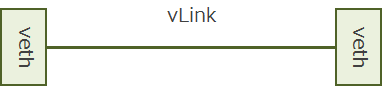
\includegraphics[scale=0.6]{img/phut-vlink-model.png}
 \caption{vLinkのモデル}
 \label{fig:vlink-model}
\end{figure}

これには「Phutで扱うための名前」と「OS上で使われる実際のデバイス名」があ
る。例えば、\verb|Phut::Link('sport', 'dport')|というコードに対しては、
\code{sport}, \code{dport}がPhutで扱うための名前となる。

Phutの内部処理で、Phutが識別するインタフェース名をもとに、OS上で使われる
実際のデバイス名(\code{L1\_sport}, \code{L1\_dport})が決められる
(\figref{fig:vlink-model2})。OS上(NetTester外)からPhutで生成したインスタ
ンスを操作する場合は、実際のデバイス名を使用する必要がある。また、デバイ
ス名として使用できる文字列には上限があるため、名前(文字列)の長さに注意す
る。\footnote{vHost/Netns の \code{:name} attribute は12文字まで。OS上で
はこれに\code{L1\_}を付与してた15文字が最大長とな
る~\cite{netns-name-max-length}。}

\begin{figure}[h]
 \centering
 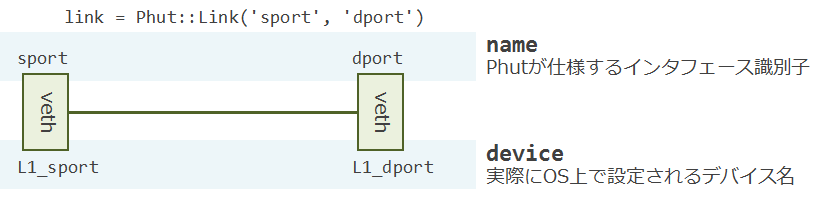
\includegraphics[scale=0.6]{img/phut-vlink-model2.png}
 \caption{インタフェースの名前とデバイス名}
 \label{fig:vlink-model2}
\end{figure}

生成した vLink(veth pair)をそのほかのインスタンス(vHost/vSwitch)に接続す
ることで仮想ネットワークを構成する。

\subsection{vHost}
Phutでは2種類のノードを取り扱う。

\paragraph{Phut::Vhost}

Rubyで実装された仮想ノードである。下記のように動作がシンプルで、直接的な
動作チェックに向いている。
\begin{itemize}
 \item UDPパケットの送受信ができる(\verb|#send_packet|)。
       \begin{itemize}
        \item ARPは送信せず、直接 IP(UDP) Unicastを送信する。
       \end{itemize}
 \item ARP処理しないので、あらかじめ ARP table を与えておく必要がある
       (\verb|arp_entries|で ``\verb|IP1/MAC1,IP2/MAC2,...|'' のような文
       字列を与える)。パケット送信(\verb|#send_packet|)するときに ARP
       entry が見つからなければ何もしない(パケットを送信しない)。
\begin{lstlisting}
arp_entries = "192.168.0.1/00:ba:dc:ab:1e:01,192.168.0.2/00:ba:dc:ab:1e:02"
\end{lstlisting}
\end{itemize}


インスタンスを作るときに、\verb|device| でこのノードに接続する veth を指
定する(\lstref{lst:create-vhost-instance})。
\begin{lstlisting}[caption=Phut::Vhostインスタンスの作成,label=lst:create-vhost-instance]
host = Phut::Vhost.create(name: 'host_name',
                          ip_address: ip_address,
                          mac_address: mac_address,
                          arp_entries: arp_entries,
                          device: link.device('interface_name'))
\end{lstlisting}

\paragraph{Phut::Netns}
Linux namespace で作成したノード。何らかのコマンド(プロセス)を namespace
上で実行する形をとる。これは、ネットワークのみノードOSから分離した
(namespaceをわけた)状態で、OS上でコマンド実行するのと同様である。実行結
果の処理などは自分で作りこみをする必要があるが、その分自由度がおおきく、
OS上で実行可能な処理は原則そのまま利用できる。

Network Namespace は Linux OS の機能であるため、NetTesterで作成した
namespace であっても、NetTester の外側(OS)から使用可能である\footnote{OS
上で \code{sudo ip netns exec <host namespace> <command>} する。}。

複雑なデバッグ作業をやりたい場合は Netns を使う必要がある。インスタンス
を作ったあと \verb|#device=| でこのノードに接続する veth を指定する
(\lstref{lst:create-netns-instance})。

\begin{lstlisting}[caption=Phut::Netnsインスタンスの作成,label=lst:create-netns-instance]
host = Phut::Netns.create(name: 'host_name',
                          ip_address: ip_address,
                          netmask: '255.255.255.0',
                          mac_address: mac_address)
host.device = link.device('interface_name')
\end{lstlisting}

\subsection{vSwitch}

NetTester自体をテストするためのテストシナリオ
\footnote{\url{https://github.com/net-tester/net-tester/blob/develop/features/step_definitions/net_tester_physical_switch_steps.rb},
\url{https://github.com/net-tester/net-tester/blob/develop/features/step_definitions/net_tester_steps.rb}}
実装の中で、NetTester本体の起動では以下のような処理をしている
(\lstref{lst:run-nettester})。
\begin{lstlisting}[caption=NetTesterの起動,label=lst:run-nettester]
 Given(/^DPID が (\S+) の NetTester 物理スイッチ$/) do |dpid|
  @physical_test_switch = PhysicalTestSwitch.create(dpid: dpid.hex)
 end

 Given(/^NetTester を起動$/) do
  main_link = Phut::Link.create('ssw', 'psw')
  NetTester.run(network_device: main_link.device(:ssw),
                physical_switch_dpid: @physical_test_switch.dpid)
  @physical_test_switch.add_numbered_port(1, main_link.device(:psw))
 end
\end{lstlisting}

これにより、\figref{fig:phut-testee-switch}のように仮想ネットワークが構
成される。ここでは、NetTester自身のテストをするために、物理スイッチに相
当するものをvSwitch(ソフトウェアスイッチ, \verb|@physical_test_switch|)
として起動している。

\begin{figure}[h]
 \centering
 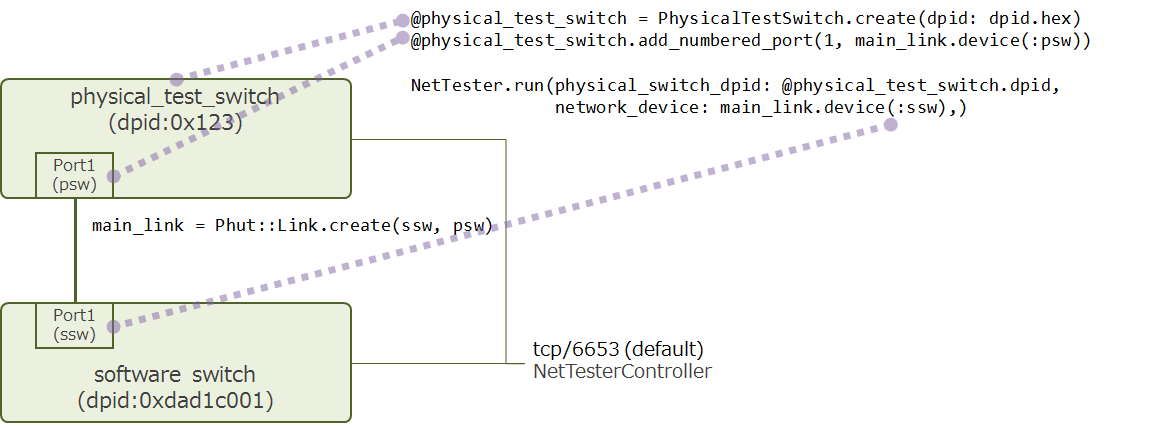
\includegraphics[scale=0.6]{img/phut-psw-ssw-model.png}
 \caption{テスト用物理スイッチ(相当)の起動と接続}
 \label{fig:phut-psw-ssw-model}
\end{figure}

\verb|NetTester.#run|の中では以下の処理をしている。

\begin{itemize}
 \item trema の起動 (NetTesterControllerの起動)
 \item ssw の起動
 \item ssw に veth (\verb|main_link.device(:ssw)|) を接続する。
       (port number 1)
\end{itemize}

\subsection{テスト対象としての vSwitch の利用}

NetTester 自身をテストする場合、テスト対象ネットワークに相当するものをテ
ストシナリオ中で用意する必要がある。テスト対象として vSwitch を起動する
場合は\lstref{lst:run-vswitch}のようにおこなう
\footnote{\url{https://github.com/net-tester/net-tester/blob/develop/features/step_definitions/ethernet_switch_steps.rb}}
。\lstref{lst:run-vswitch}では、テスト対象として使用する vSwitch の起動
およびコントローラとの接続(Learning Switchとして動作させるため)をおこなっ
ている。

\begin{lstlisting}[caption=vSwitchの起動,label=lst:run-vswitch]
Given(/^テスト対象のイーサネットスイッチ$/) do
  @testee_switch = TesteeSwitch.create(dpid: 0x1, tcp_port: 6654)
  step %(I successfully run `trema run ../../vendor/learning_switch/lib/learning_switch.rb --port 6654 -L #{Phut.log_dir} -P #{Phut.pid_dir} -S #{Phut.socket_dir} --daemon`)
end
\end{lstlisting}

テストシナリオ内部
\footnote{\url{https://github.com/net-tester/net-tester/blob/develop/features/step_definitions/net_tester_physical_switch_steps.rb}}
では、テスト対象ネットワーク(\verb|@testee_switch|)と物理スイッチ
(\verb|@physical_test_switch|)を接続するため、
\lstref{lst:connect-vswitch}のような処理をおこなう。

\begin{lstlisting}[caption=vSwitch間接続,label=lst:connect-vswitch]
Given(/^NetTester 物理スイッチとテスト対象のスイッチを次のように接続:$/) do |table|
  table.hashes.each do |each|
    pport_id = each['Physical Port'].to_i
    tport_id = each['Testee Port'].to_i
    port_name = "pport#{pport_id}"
    tport_name = "tport#{tport_id}"
    link = Phut::Link.create(tport_name, port_name)
    @physical_test_switch.add_numbered_port(pport_id, link.device(port_name))
    @testee_switch.add_numbered_port(tport_id, link.device(tport_name))
  end
end
\end{lstlisting}

これによって\figref{fig:phut-testee-switch}のように仮想ネットワークが構
成される。

\begin{figure}[h]
 \centering
 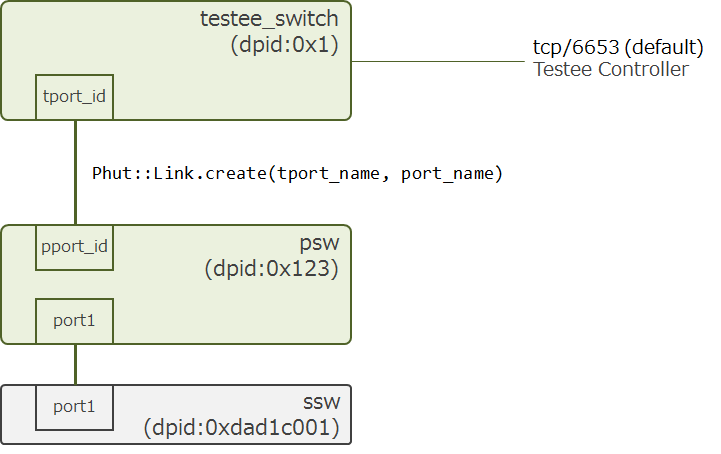
\includegraphics[scale=0.6]{img/phut-testee-switch.png}
 \caption{テスト対象機器(スイッチ)の生成と接続}
 \label{fig:phut-testee-switch}
\end{figure}

\subsection{テスト対象としての vHost の利用}

ポート間パッチのテスト
\footnote{\url{https://github.com/net-tester/net-tester/blob/develop/features/internal_tests/p2p_patch.feature}}
では、テスト対象ネッNetTesterのテストシナリオネットワークに属するノード
の生成・操作は\lstref{lst:create-testnode}のように記述している。

\begin{lstlisting}[caption=テスト用ノードの生成,label=lst:create-testnode]
  Background:
    Given DPID が 0x123 の NetTester 物理スイッチ
    And NetTester を起動
    And NetTester 物理スイッチとテスト対象ノードを次のように接続:
      | Physical Port | Host |
      |             2 |    1 |
      |             3 |    2 |
      |             4 |    3 |
\end{lstlisting}

テストシナリオ内部
\footnote{\url{https://github.com/net-tester/net-tester/blob/develop/features/step_definitions/p2p_patch_steps.rb}}(\lstref{lst:operate-testnode})
では、テストシナリオ(\lstref{lst:create-testnode})で与えられたパラメタを
元に、次のようにノードを生成してテストを実行する。

\begin{lstlisting}[caption=テスト用ノードの生成と操作,label=lst:operate-testnode]
Given(/^NetTester 物理スイッチとテスト対象ノードを次のように接続:$/) do |table|
  ip_of_host = {}
  mac_of_host = {}
  vhost_arp_list = []

  table.hashes.each do |each|
    host_id = each['Host']
    ip_address = "192.168.0.#{host_id}"
    ip_of_host[host_id] = ip_address
    mac_address = "00:ba:dc:ab:1e:#{sprintf('%02x', host_id)}"
    mac_of_host[host_id] = mac_address
    vhost_arp_list.append "#{ip_address}/#{mac_address}"
  end

  arp_entries = vhost_arp_list.join(',')
  table.hashes.each do |each|
    pport_id = each['Physical Port'].to_i
    pport_name = "pport#{pport_id}"
    host_id = each['Host']
    host_name = "host#{host_id}"
    link = Phut::Link.create(host_name, pport_name)
    Phut::Vhost.create(name: host_name,
                       ip_address: ip_of_host[host_id],
                       mac_address: mac_of_host[host_id],
                       device: link.device(host_name),
                       arp_entries: arp_entries)
    @physical_test_switch.add_numbered_port(pport_id, link.device(pport_name))
  end
end
\end{lstlisting}

\lstref{lst:operate-testnode}では\verb|Phut::Vhost|を使用している。すべ
てのテスト用ノードの \verb|arp_entries| を作るために IP/MAC を用意すると
ころと、Phut instance を生成するパートに分割している。これにより、
\figref{fig:phut-testee-host}のように複数のテスト用ノードが作成され、テ
スト対象ネットワークとして物理スイッチ(\verb|psw|)に接続される。

\begin{figure}[h]
 \centering
 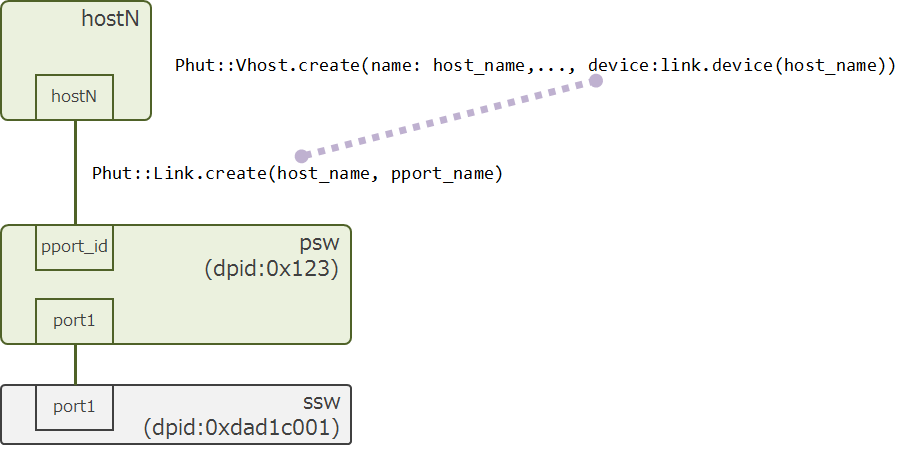
\includegraphics[scale=0.6]{img/phut-testee-host.png}
 \caption{テスト対象機器(ノード)の生成と接続}
 \label{fig:phut-testee-host}
\end{figure}

%%% Local Variables:
%%% mode: yatex
%%% TeX-master: "main.tex"
%%% End:

%% -*- coding: utf-8-unix -*-

\chapter{テストシナリオ実装時のトラブルとワークアラウンド}
ネットワークのテストという観点で実際に発見できた問題点については
\ref{sec:statictest-founded-issues}節でとりあげている。本章では、テスト
シナリオ実装の際におきた問題点やワークアラウンドについて解説する。こうし
たワークアラウンドは、事情や理由がわからないと冗長あるいは不合理にみえる
ことがあるため、理由をふくめたノウハウを共有しておくことは重要である。

本章では特に、テストを繰り返し実行すると成功・失敗がくりかえされ、結果が
不定になった事例を選定している。こうしたテストは flaky\footnote{flaky =
当てにならない。} test とも呼ばれ、テストの連続実行(回帰テスト)において
問題となる。

 \section{初回のping送受信失敗}
 \label{sec:ping-probrem}

    \paragraph{事象}
L3の通信試験(\code{ping}コマンド)で、最初の1パケット(場合によっては数パ
ケット)だけ送受信に失敗する。そのため、テスト実行ごとにコマンド実行結果
(ping packet loss)判定が変化して、テストが成功したり失敗したりする。

    \paragraph{原因と対処}
テスト対象が物理ネットワークであるため、ARP cache 等その時々のネットワー
ク状態による結果のゆらぎが発生してしまう。よく知られたワークアラウンドと
しては、テスト実行のまえに、予備的なパケット送受信をおこなって、テスト対
象ネットワーク内の状態を更新しておくことである。本プロジェクトでも、
\lstref{lst:ping-workaround}のように ping packet loss 測定前に ping を1
パケット送受信しておく\footnote{本プロジェクトではこれを「捨てping」と呼
んでいる。}ことで回避している~\cite{examples-pr49}。

\begin{lstlisting}[caption=予備的ping実行の例,label=lst:ping-workaround,linebackgroundcolor={\ifnum\value{lstnumber}=3 \color{green!30}\fi}]
When(/^ヨーヨーダイン社内部のユーザ PC に ping$/) do
  cd('.') do
    @src_host.exec "bash -c 'ping #{@user_pc.ip_address} -c 1; exit 0'"
    @src_host.exec "ping #{@user_pc.ip_address} -c 4 > log/ping.log"
  end
end
\end{lstlisting}

 \section{Netcat/telnetコマンドのデータ送受信順序}
 \label{sec:telnet-probrem}

    \paragraph{事象}
Telentを使った通信試験において、\lstref{lst:telnet-bk}に示すようにテスト
が10回に1回程度しか成功しないという現象が発生した。テストではのように、
サーバとして netcat (\code{nc}コマンド)、クライアントとして
\code{telnet} コマンドを使用している。
 
\begin{lstlisting}[caption=Telnetテストシナリオ,label=lst:telnet-bk]
tajima@nettester_2nd:~/repo/examples-tjmtrhs$ bundle exec cucumber features/telnet_internal_network.feature
@static
Feature: 社内テスト環境設定  ヨーヨーダイン社の開発者として、
社内テストサーバにアクセスしたい  なぜならテスト環境設定を行う必要があるから
Scenario: 社内テストサーバへアクセス            # features/telnet_internal_network.feature:8
Given ヨーヨーダイン社内部のテスト環境サーバ        # features/step_definitions/virtual_host.rb:14
 And ヨーヨーダイン社内部のクライアント            # features/step_definitions/virtual_host.rb:6
When 開発者 PC からテストサーバへTelnetでアクセス # features/step_definitions/telnet_steps.rb:2
 Then 社内テストサーバにアクセス成功             # features/step_definitions/telnet_steps.rb:20
expected "Trying 10.10.10.2...\nConnected to 10.10.10.2.\nEscape character is '^]'." to have file content: string includes: "TelnetOK" (RSpec::Expectations::ExpectationNotMetError)
     ./features/step_definitions/telnet_steps.rb:21:in `/^社内テストサーバにアクセス成功$/'      features/telnet_internal_network.feature:12:in `Then 社内テストサーバにアクセス成功' Failing Scenarios: cucumber features/telnet_internal_network.feature:8 #
 Scenario: 社内テストサーバへアクセス 1 scenario (1 failed) 4 steps (1 failed, 3 passed) 0m10.610s
\end{lstlisting}

    \paragraph{調査}

原因を調査するために、同様の操作を手動で実行した場合(成功する場合)とテス
トシナリオ実行で失敗する場合のそれぞれについて strace による調査を実施し
た。\lstref{lst:telnet-success}に成功時、\lstref{lst:telnet-fail}に失敗
時の strace ログを示す。どちらも前半部分は省略してあり、\code{connect}
から 終了(\code{exit})までのログを抜粋してある。

\begin{lstlisting}[caption=Telnet成功時(手動),label=lst:telnet-success,linebackgroundcolor={\ifnum\value{lstnumber}>22 \ifnum\value{lstnumber}<29\color{green!30}\fi\fi}]
socket(PF_INET, SOCK_STREAM, IPPROTO_IP) = 3
setsockopt(3, SOL_IP, IP_TOS, [16], 4)  = 0
connect(3, {sa_family=AF_INET, sin_port=htons(8080), sin_addr=inet_addr("192.168.20.166")}, 16) = 0
open("/etc/telnetrc", O_RDONLY)         = -1 ENOENT (No such file or directory)
open("/home/nwtestsys/.telnetrc", O_RDONLY) = -1 ENOENT (No such file or directory)
write(1, "Trying 192.168.20.166...\nConnect"..., 80Trying 192.168.20.166...
Connected to 192.168.20.166.
Escape character is '^]'.
) = 80
rt_sigprocmask(SIG_BLOCK, NULL, [], 8)  = 0
rt_sigaction(SIGINT, {0x407fe0, [INT], SA_RESTORER|SA_RESTART, 0x7fa39fd524a0}, {SIG_DFL, [], 0}, 8) = 0
rt_sigaction(SIGQUIT, {0x407f90, [QUIT], SA_RESTORER|SA_RESTART, 0x7fa39fd524a0}, {SIG_DFL, [], 0}, 8) = 0
rt_sigaction(SIGWINCH, {0x407f70, [WINCH], SA_RESTORER|SA_RESTART, 0x7fa39fd524a0}, {SIG_DFL, [], 0}, 8) = 0
rt_sigaction(SIGTSTP, {0x40c4b0, [TSTP], SA_RESTORER|SA_RESTART, 0x7fa39fd524a0}, {0x40c4b0, [TSTP], SA_RESTORER|SA_RESTART, 0x7fa39fd524a0}, 8) = 0
ioctl(0, TCGETS, {B38400 opost isig icanon echo ...}) = 0
ioctl(0, SNDCTL_TMR_STOP or TCSETSW, {B38400 opost isig icanon echo ...}) = 0
ioctl(0, TCGETS, {B38400 opost isig icanon echo ...}) = 0
ioctl(0, FIONBIO, [1])                  = 0
ioctl(1, FIONBIO, [1])                  = 0
ioctl(3, FIONBIO, [1])                  = 0
setsockopt(3, SOL_SOCKET, SO_OOBINLINE, [1], 4) = 0
select(4, [0 3], [], [3], {0, 0})       = 1 (in [3], left {0, 0})
recvfrom(3, "TelnetOK\n", 8191, 0, NULL, NULL) = 9
select(4, [0 3], [1], [3], {0, 0})      = 2 (in [3], out [1], left {0, 0})
write(1, "TelnetOK\n", 9TelnetOK
)               = 9
recvfrom(3, "", 8183, 0, NULL, NULL)    = 0
rt_sigaction(SIGTSTP, {SIG_DFL, [TSTP], SA_RESTORER|SA_RESTART, 0x7fa39fd524a0}, {0x40c4b0, [TSTP], SA_RESTORER|SA_RESTART, 0x7fa39fd524a0}, 8) = 0
ioctl(0, TCGETS, {B38400 opost isig icanon echo ...}) = 0
ioctl(0, SNDCTL_TMR_STOP or TCSETSW, {B38400 opost isig icanon echo ...}) = 0
ioctl(0, TCGETS, {B38400 opost isig icanon echo ...}) = 0
ioctl(0, FIONBIO, [0])                  = 0
ioctl(1, FIONBIO, [0])                  = 0
close(3)                                = 0
rt_sigaction(SIGTSTP, {0x40c4b0, [TSTP], SA_RESTORER|SA_RESTART, 0x7fa39fd524a0}, {SIG_DFL, [TSTP], SA_RESTORER|SA_RESTART, 0x7fa39fd524a0}, 8) = 0
ioctl(0, TCGETS, {B38400 opost isig icanon echo ...}) = 0
ioctl(0, SNDCTL_TMR_STOP or TCSETSW, {B38400 opost isig icanon echo ...}) = 0
ioctl(0, TCGETS, {B38400 opost isig icanon echo ...}) = 0
ioctl(0, FIONBIO, [1])                  = 0
ioctl(1, FIONBIO, [1])                  = 0
select(2, NULL, [1], NULL, NULL)        = 1 (out [1])
rt_sigaction(SIGTSTP, {SIG_DFL, [TSTP], SA_RESTORER|SA_RESTART, 0x7fa39fd524a0}, {0x40c4b0, [TSTP], SA_RESTORER|SA_RESTART, 0x7fa39fd524a0}, 8) = 0
ioctl(0, TCGETS, {B38400 opost isig icanon echo ...}) = 0
ioctl(0, SNDCTL_TMR_STOP or TCSETSW, {B38400 opost isig icanon echo ...}) = 0
ioctl(0, TCGETS, {B38400 opost isig icanon echo ...}) = 0
ioctl(0, FIONBIO, [0])                  = 0
ioctl(1, FIONBIO, [0])                  = 0
rt_sigaction(SIGTSTP, {0x40c4b0, [TSTP], SA_RESTORER|SA_RESTART, 0x7fa39fd524a0}, {SIG_DFL, [TSTP], SA_RESTORER|SA_RESTART, 0x7fa39fd524a0}, 8) = 0
ioctl(0, TCGETS, {B38400 opost isig icanon echo ...}) = 0
ioctl(0, SNDCTL_TMR_STOP or TCSETSW, {B38400 opost isig icanon echo ...}) = 0
ioctl(0, TCGETS, {B38400 opost isig icanon echo ...}) = 0
ioctl(0, FIONBIO, [1])                  = 0
ioctl(1, FIONBIO, [1])                  = 0
select(2, NULL, [1], NULL, NULL)        = 1 (out [1])
rt_sigaction(SIGTSTP, {SIG_DFL, [TSTP], SA_RESTORER|SA_RESTART, 0x7fa39fd524a0}, {0x40c4b0, [TSTP], SA_RESTORER|SA_RESTART, 0x7fa39fd524a0}, 8) = 0
ioctl(0, TCGETS, {B38400 opost isig icanon echo ...}) = 0
ioctl(0, SNDCTL_TMR_STOP or TCSETSW, {B38400 opost isig icanon echo ...}) = 0
ioctl(0, TCGETS, {B38400 opost isig icanon echo ...}) = 0
ioctl(0, FIONBIO, [0])                  = 0
ioctl(1, FIONBIO, [0])                  = 0
write(2, "Connection closed by foreign hos"..., 35Connection closed by foreign host.
) = 35
close(-1)                               = -1 EBADF (Bad file descriptor)
exit_group(1)                           = ?
+++ exited with 1 +++
\end{lstlisting}

\begin{lstlisting}[caption=Telnet失敗時,label=lst:telnet-fail,linebackgroundcolor={\ifnum\value{lstnumber}>24 \ifnum\value{lstnumber}<26\color{green!30}\fi\fi}]
socket(PF_INET, SOCK_STREAM, IPPROTO_IP) = 3
setsockopt(3, SOL_IP, IP_TOS, [16], 4)  = 0
connect(3, {sa_family=AF_INET, sin_port=htons(23), sin_addr=inet_addr("10.10.10.2")}, 16) = 0
open("/etc/telnetrc", O_RDONLY)         = -1 ENOENT (No such file or directory)
open("/root/.telnetrc", O_RDONLY)       = -1 ENOENT (No such file or directory)

write(1, "Trying 10.10.10.2...\nConnected t"..., 72Trying 10.10.10.2...
Connected to 10.10.10.2.
Escape character is '^]'.
) = 72
rt_sigprocmask(SIG_BLOCK, NULL, [], 8)  = 0
rt_sigaction(SIGINT, {0x407fe0, [INT], SA_RESTORER|SA_RESTART, 0x7fdd72e1d4a0}, {SIG_DFL, [], 0}, 8) = 0
rt_sigaction(SIGQUIT, {0x407f90, [QUIT], SA_RESTORER|SA_RESTART, 0x7fdd72e1d4a0}, {SIG_DFL, [], 0}, 8) = 0
rt_sigaction(SIGWINCH, {0x407f70, [WINCH], SA_RESTORER|SA_RESTART, 0x7fdd72e1d4a0}, {SIG_DFL, [], 0}, 8) = 0
rt_sigaction(SIGTSTP, {0x40c4b0, [TSTP], SA_RESTORER|SA_RESTART, 0x7fdd72e1d4a0}, {0x40c4b0, [TSTP], SA_RESTORER|SA_RESTART, 0x7fdd72e1d4a0}, 8) = 0
ioctl(0, TCGETS, 0x7ffc1c8e01d0)        = -1 ENOTTY (Inappropriate ioctl for device)
ioctl(0, SNDCTL_TMR_STOP or TCSETSW, {B0 opost isig icanon echo ...}) = -1 ENOTTY (Inappropriate ioctl for device)
ioctl(0, TCGETS, 0x7ffc1c8e01d0)        = -1 ENOTTY (Inappropriate ioctl for device)
ioctl(0, SNDCTL_TMR_START or TCSETS, {B0 opost isig icanon echo ...}) = -1 ENOTTY (Inappropriate ioctl for device)
ioctl(0, FIONBIO, [1])                  = 0
ioctl(1, FIONBIO, [1])                  = 0
ioctl(3, FIONBIO, [1])                  = 0
setsockopt(3, SOL_SOCKET, SO_OOBINLINE, [1], 4) = 0
select(4, [0 3], [3], [3], {0, 0})      = 2 (in [0], out [3], left {0, 0})
sendto(3, "\377\375\3\377\373\30\377\373\37\377\373 \377\373!\377\373\"\377\373'\377\375\5", 24, 0, NULL, 0) = 24
read(0, "", 8191)                       = 0
ioctl(0, TCGETS, 0x7ffc1c8e01a0)        = -1 ENOTTY (Inappropriate ioctl for device)
rt_sigaction(SIGTSTP, {SIG_DFL, [TSTP], SA_RESTORER|SA_RESTART, 0x7fdd72e1d4a0}, {0x40c4b0, [TSTP], SA_RESTORER|SA_RESTART, 0x7fdd72e1d4a0}, 8) = 0
ioctl(0, TCGETS, 0x7ffc1c8e01f0)        = -1 ENOTTY (Inappropriate ioctl for device)
ioctl(0, SNDCTL_TMR_STOP or TCSETSW, {B0 -opost -isig -icanon -echo ...}) = -1 ENOTTY (Inappropriate ioctl for device)
ioctl(0, TCGETS, 0x7ffc1c8e01f0)        = -1 ENOTTY (Inappropriate ioctl for device)
ioctl(0, SNDCTL_TMR_START or TCSETS, {B0 -opost -isig -icanon -echo ...}) = -1 ENOTTY (Inappropriate ioctl for device)
ioctl(0, FIONBIO, [0])                  = 0
ioctl(1, FIONBIO, [0])                  = 0
close(3)                                = 0
rt_sigaction(SIGTSTP, {0x40c4b0, [TSTP], SA_RESTORER|SA_RESTART, 0x7fdd72e1d4a0}, {SIG_DFL, [TSTP], SA_RESTORER|SA_RESTART, 0x7fdd72e1d4a0}, 8) = 0
ioctl(0, TCGETS, 0x7ffc1c8e01c0)        = -1 ENOTTY (Inappropriate ioctl for device)
ioctl(0, SNDCTL_TMR_STOP or TCSETSW, {B0 opost -isig -icanon echo ...}) = -1 ENOTTY (Inappropriate ioctl for device)
ioctl(0, TCGETS, 0x7ffc1c8e01c0)        = -1 ENOTTY (Inappropriate ioctl for device)
ioctl(0, SNDCTL_TMR_START or TCSETS, {B0 opost -isig -icanon echo ...}) = -1 ENOTTY (Inappropriate ioctl for device)
ioctl(0, FIONBIO, [1])                  = 0
ioctl(1, FIONBIO, [1])                  = 0
select(2, NULL, [1], NULL, NULL)        = 1 (out [1])
rt_sigaction(SIGTSTP, {SIG_DFL, [TSTP], SA_RESTORER|SA_RESTART, 0x7fdd72e1d4a0}, {0x40c4b0, [TSTP], SA_RESTORER|SA_RESTART, 0x7fdd72e1d4a0}, 8) = 0
ioctl(0, TCGETS, 0x7ffc1c8e01c0)        = -1 ENOTTY (Inappropriate ioctl for device)
ioctl(0, SNDCTL_TMR_STOP or TCSETSW, {B0 -opost -isig -icanon -echo ...}) = -1 ENOTTY (Inappropriate ioctl for device)
ioctl(0, TCGETS, 0x7ffc1c8e01c0)        = -1 ENOTTY (Inappropriate ioctl for device)
ioctl(0, SNDCTL_TMR_START or TCSETS, {B0 -opost -isig -icanon -echo ...}) = -1 ENOTTY (Inappropriate ioctl for device)
ioctl(0, FIONBIO, [0])                  = 0
ioctl(1, FIONBIO, [0])                  = 0
rt_sigaction(SIGTSTP, {0x40c4b0, [TSTP], SA_RESTORER|SA_RESTART, 0x7fdd72e1d4a0}, {SIG_DFL, [TSTP], SA_RESTORER|SA_RESTART, 0x7fdd72e1d4a0}, 8) = 0
ioctl(0, TCGETS, 0x7ffc1c8e01c0)        = -1 ENOTTY (Inappropriate ioctl for device)
ioctl(0, SNDCTL_TMR_STOP or TCSETSW, {B0 opost -isig -icanon echo ...}) = -1 ENOTTY (Inappropriate ioctl for device)
ioctl(0, TCGETS, 0x7ffc1c8e01c0)        = -1 ENOTTY (Inappropriate ioctl for device)
ioctl(0, SNDCTL_TMR_START or TCSETS, {B0 opost -isig -icanon echo ...}) = -1 ENOTTY (Inappropriate ioctl for device)
ioctl(0, FIONBIO, [1])                  = 0
ioctl(1, FIONBIO, [1])                  = 0
select(2, NULL, [1], NULL, NULL)        = 1 (out [1])
rt_sigaction(SIGTSTP, {SIG_DFL, [TSTP], SA_RESTORER|SA_RESTART, 0x7fdd72e1d4a0}, {0x40c4b0, [TSTP], SA_RESTORER|SA_RESTART, 0x7fdd72e1d4a0}, 8) = 0
ioctl(0, TCGETS, 0x7ffc1c8e01d0)        = -1 ENOTTY (Inappropriate ioctl for device)
ioctl(0, SNDCTL_TMR_STOP or TCSETSW, {B0 -opost -isig -icanon -echo ...}) = -1 ENOTTY (Inappropriate ioctl for device)
ioctl(0, TCGETS, 0x7ffc1c8e01d0)        = -1 ENOTTY (Inappropriate ioctl for device)
ioctl(0, SNDCTL_TMR_START or TCSETS, {B0 -opost -isig -icanon -echo ...}) = -1 ENOTTY (Inappropriate ioctl for device)
ioctl(0, FIONBIO, [0])                  = 0
ioctl(1, FIONBIO, [0])                  = 0
write(2, "Connection closed by foreign hos"..., 35Connection closed by foreign host.
) = 35
close(-1)                               = -1 EBADF (Bad file descriptor)
exit_group(1)                           = ?
+++ exited with 1 +++
\end{lstlisting}

成功時(\lstref{lst:telnet-success})では、\code{connect}後にサーバからの
\verb|recvfrom(3, "TelnetOK\n", ...)|が先にきている(23行目)。しかし、失
敗時(\lstref{lst:telnet-fail})では、クライアントからのネゴシエーションの
\verb|sendto(3, "\377...", ...)|が先に実行されている(25行目)。この場合後
続の\code{write}は実行されていない(そもそも\code{recv}しない)。

これらの strace ログから、送受信順序によるものと仮定した。仮定を実証する
ために、telnetクライアントを改変する。Telnetクライアントが\code{connect}
したあとサーバから来るデータを先に受ける(\code{recv})ために、
\code{connect}のあとに\code{sleep}を入れる
(\lstref{lst:modified-telnet-client})。これをビルドして
(\lstref{lst:howto-build-telnet})、テストステップの中で使用する
(\lstref{lst:telnet-step})。結果として、エラーが発生しなくなることを確認
できた。

\begin{lstlisting}[caption=telnetクライアント改変,label=lst:modified-telnet-client]
--- netkit-telnet-0.17/telnet/netlink.cc        2017-03-21 00:30:45.990808011 +0900
+++ netkit-telnet-0.17-mod/telnet/netlink.cc    2017-03-21 00:24:45.178808011 +0900
@@ -158,6 +158,7 @@
     if (::connect(net, addr->ai_addr, addr->ai_addrlen) < 0) {
        return 1;
     }
+    sleep(10);
     return 2;
 }
\end{lstlisting}

\begin{lstlisting}[caption=telnetクライアントのビルド手順,label=lst:howto-build-telnet]
sudo echo "deb http://gb.archive.ubuntu.com/ubuntu/ xenial main restricted" | sudo tee -a /etc/apt/sources.list
sudo echo "deb-src http://gb.archive.ubuntu.com/ubuntu/ xenial main restricted" | sudo tee -a /etc/apt/sources.list
sudo apt-get source telnet
sudo apt-get install libncurses-dev
cd netkit-telnet-0.17
./configure
cd telnet
make
\end{lstlisting}

\begin{lstlisting}[caption=改変telnetクライアントの使用,label=lst:telnet-step]
When(/^ヨーヨーダイン社内部のテスト環境サーバに telnet でログイン$/) do
  cd('.') do
    @telnet_service = AsyncExecutor.new(host: @test_host, result_file: 'log/telnet_server.log')
    @telnet_service.exec "bash -c 'echo LoginOK | sudo nc -l 23'"
    @src_host.exec "bash -c '/home/nwtestsys/examples/telnet-source/netkit-telnet-0.17/telnet/telnet #{@test_host.ip_address} > log/login.log; exit 0'"
  end
end
\end{lstlisting}

    \paragraph{結果と対処}
当初、netcat をサーバとして使用していた。サーバはクライアントからの接続
を受け付けて echo するとすぐに切断する。結果としてサーバから送られたデー
タの \code{recv} とクライアントが送るデータの \code{sendto} のどちらが早
いかという順序(タイミング)問題が発生していたと考えられる。

こうした問題はサーバ側に telnet daemon (telnetd) を使用することで回避可
能である。しかし、telnetd を使用すると対話的処理(expect)が必要になってし
まうため、テストステップが複雑になる。そこで、クライアント側に
Net::Telnet を使用することで問題を回避している
(\lstref{lst:telnet-step-new})。

\begin{lstlisting}[caption=修正後テストステップ,label=lst:telnet-step-new]
When(/^社内のテスト環境サーバに telnet でログイン$/) do
  cd('.') do
    @telnet_service = AsyncExecutor.new(host: @test_host, result_file: 'log/telnet_host.log')
    @telnet_service.exec "bash -c 'echo LoginOK | sudo nc -l 23'"
    @src_host.exec "ruby -e \"require 'net/telnet'; Net::Telnet.new('Host' => '#{@test_host.ip_address}', 'Port' => '23').cmd('') {|res| print res}\" > log/login.log"
  end
end
\end{lstlisting}

%%% Local Variables:
%%% mode: yatex
%%% TeX-master: "main.tex"
%%% End:

%% -*- coding: utf-8-unix -*-

\begin{thebibliography}{99}
 \bibitem{ool-web}
         ``一般社団法人沖縄オープンラボラトリ \verb+|+ Okinawa Open Laboratory'',
         \url{http://www.okinawaopenlabs.org/}
 \bibitem{ool-l1pj-web}
         ``L1Patch応用NWテストシステム プロジェクト'',
         \url{http://www.okinawaopenlabs.org/archives/research2014/150410}
 \bibitem{l1pjpoc}
         ``L1patch応用ネットワークテストシステム 試験結果レポート''.
         \url{https://github.com/oolorg/ool-l1patch-dev/blob/master/report/l1pj-poc-report-20151114.pdf}.
         2015.
 \bibitem{l1pjtech}
         ``L1patch応用ネットワークテストシステム 技術レポート''.
         \url{https://github.com/oolorg/ool-l1patch-dev/blob/master/report/l1pj-tech-report-20151114.pdf}.
         2015.
 \bibitem{ool-testbedpj}
         ``OF-Patch拡張 プロジェクト'',
         \url{https://www.okinawaopenlabs.org/archives/research2014/141006}
 \bibitem{ool-vnftestpj}
         田部英樹, ``VNFテストシナリオ自動化PJについて'',
         \url{https://www.okinawaopenlabs.org/wp/wp-content/uploads/8_VNF%E3%83%86%E3%82%B9%E3%83%88%E3%82%B7%E3%83%8A%E3%83%AA%E3%82%AA%E8%87%AA%E5%8B%95%E5%8C%96%E3%83%97%E3%83%AD%E3%82%B8%E3%82%A7%E3%82%AF%E3%83%88%E3%81%AB%E3%81%A4%E3%81%84%E3%81%A6.pdf}, 2015.
 \bibitem{wbsw-oss-test-automation}
         渋谷惠美, 川上秀彦, 長谷川輝之, 山口弘純, ``ホワイトボックスス
         イッチとOSSを活用したネットワークに対する検証自動化システム設計
         に関する一提案'', 信学技報, vol. 116, no. 111, NS2016-34,
         pp. 35--40, 2016年6月.
 \bibitem{needlework-web}
         ``NEEDLEWORK \verb+|+ AP Communications'',
         \url{http://www.ap-com.co.jp/ja/needlework/}
 \bibitem{needlework-slide}
         鈴木飛鳥,``FWのポリシーテストを自動化してみた'',
         \url{https://www.slideshare.net/tanksuzuki/fw-59102915},
         NetOpsCoding\#2, 2016.
 \bibitem{infratester-github}
         ``Infrataster by ryotarai'',
         \url{http://infrataster.net/}
 \bibitem{todd-github}
         ``toddproject/todd: A highly extensible framework for distributed capacity and connectivity testing (Testing on Demand....Distributed!)'',
         \url{https://github.com/toddproject/todd}
 \bibitem{todd-blog}
         ``The Power of Test-Driven Network Automation'',
         \url{https://keepingitclassless.net/2016/03/test-driven-network-automation/}
 \bibitem{openvnet-web}
         ``OpenVNet'', \url{https://openvnet.org/}
 \bibitem{openvnet-slide}
         山崎泰宏, ``OpenVNet - SDNで物理ネットワークアプライアンスをプ
         ロビジョニングしよう'',
         \url{https://www.slideshare.net/yasuhiro_yamazaki/openvnet-sdn},
         ネットワークプログラマビリティ勉強会\#10, 2016.
 \bibitem{network-testing-sdn-atmarkit}
         村木暢哉, ``SDNで始めるネットワークの運用改善(2):SDNで物理ネッ
         トワークのテストを楽にする方法 (1/4) - @IT'',
         \url{http://www.atmarkit.co.jp/ait/articles/1612/27/news014.html},
         @IT, 2017.
 \bibitem{netmiko-github}
         ``ktbyers/netmiko: Multi-vendor library to simplify Paramiko SSH connections to network devices'',
         \url{https://github.com/ktbyers/netmiko}
 \bibitem{trigger-github}
         ``trigger/trigger: Trigger is a robust network automation toolkit written in Python that was designed for interfacing with network devices.'',
         \url{https://github.com/trigger/trigger}
 \bibitem{napalm-github}
         ``napalm-automation/napalm: Network Automation and Programmability Abstraction Layer with Multivendor support'',
         \url{https://github.com/napalm-automation/napalm}
 \bibitem{ansible-web}
         ``Ansible is Simple IT Automation'',
         \url{https://www.ansible.com/}
 \bibitem{ansible-22-news}
         ``Ansible 2.2、コンテナ、ネットワーク、クラウドサービス向けの新自動化機能を提供'',
         \url{https://www.redhat.com/ja/about/rhjapan-press-releases/ansible-22-delivers-new-automation-capabilities-containers-networks-and-cloud-services}
 \bibitem{openconfig}
         ``OpenConfig - Home'',
         \url{http://www.openconfig.net/}
 \bibitem{openconfig-news}
         ``OpenConfig - News'',
         \url{http://www.openconfig.net/news/}
 \bibitem{bdd-cycle-figref}
         ``Should TDD and BDD be used in conjunction? - Stack Overflow'',
         \url{http://stackoverflow.com/questions/33746804/should-tdd-and-bdd-be-used-in-conjunction}
 \bibitem{nettester}
         ``net-tester/net-tester: 物理ネットワークのための受け入れテストツール'',
         \url{https://github.com/net-tester/net-tester}.
 \bibitem{nettester-ex}
         ``net-tester/examples: NetTester用のサンプルテストコード'',
         \url{https://github.com/net-tester/examples}
 \bibitem{nettester-demo-movie}
         ``NetTesterでテスト自動化!~Network Test System Project~ - YouTube'',
         \url{https://www.youtube.com/watch?v=C7z3aaWgsf4}
 \bibitem{wikipedia-bdd}
         ``ビヘイビア駆動開発 - Wikipedia'',
         \url{https://ja.wikipedia.org/wiki/%E3%83%93%E3%83%98%E3%82%A4%E3%83%93%E3%82%A2%E9%A7%86%E5%8B%95%E9%96%8B%E7%99%BA}.
 \bibitem{nettester-pry}
         ``NetTesterでad-hocなテスト作業を拡張する - Qiita'',
         \url{http://qiita.com/corestate55/items/d6a8cdc03de09a46877c}
 \bibitem{ovs-vswitchd-doc}
         ``ovs-vswitchd.conf.db.5.txt'',
         \url{http://openvswitch.org/support/dist-docs/ovs-vswitchd.conf.db.5.txt}
 \bibitem{ovs-backoff-doc}
         ``[ovs-discuss] Forcing Switch to Reconnect'',
         \url{https://mail.openvswitch.org/pipermail/ovs-discuss/2012-January/006368.html}
 \bibitem{iproute2-doc}
         ``ip-netns(8) - Linux manual page'',
         \url{http://man7.org/linux/man-pages/man8/ip-netns.8.html}
 \bibitem{build-essential-doc}
         ``Ubuntu – xenial の build-essential パッケージに関する詳細'',
         \url{http://packages.ubuntu.com/ja/xenial/build-essential}
 \bibitem{rbenv}
         ``rbenv/rbenv: Groom your app’s Ruby environment'',
         \url{https://github.com/rbenv/rbenv}
 \bibitem{pry}
         ``pry/pry: An IRB alternative and runtime developer console'',
         \url{https://github.com/pry/pry}
 \bibitem{net-tester-pr7} ``implement a work-around of tcp checksum
         error in vlan trunk · Pull Request \#7 ·
         net-tester/net-tester'',
         \url{https://github.com/net-tester/net-tester/pull/7}
 \bibitem{rspec-book} David Chelimsky, Dave Astels , Zach Dennis ``The
         RSpec Book'', 株式会社クイープ(訳), 角谷信太郎, 豊田祐司(監修),
         Professional Ruby Series, 翔泳社, 2012.
 \bibitem{spiral-workflow}
         ``クライアントの要望にこたえるWebサービス開発 ~「らせん型ワークフロー」のススメ~''.
         \url{http://www.slideshare.net/mayuco/css-nite-in-sapporo-vol5-14085124}
 \bibitem{j3g14-packet-forwarding}
         吉田友哉, 松崎吉伸,
         ``幸せなパケット転送 ○○編'',
         \url{https://www.janog.gr.jp/meeting/janog14/src/janog14-yoshida-maz.pdf},
         Janog14, 2004.
 \bibitem{yoyodyne}
         ``ヨーヨーダイン - Wikipedia'',
         \url{https://ja.wikipedia.org/wiki/\%E3\%83\%A8\%E3\%83\%BC\%E3\%83\%A8\%E3\%83\%BC\%E3\%83\%80\%E3\%82\%A4\%E3\%83\%B3}
 \bibitem{h25nwsp}
         IPA 独立行政法人 情報処理推進機構,
         ``平成25年度 秋季 ネットワークスペシャリスト試験 午後I問題'',
         \url{https://www.jitec.ipa.go.jp/1_04hanni_sukiru/mondai_kaitou_2013h25_2/2013h25a_nw_pm1_qs.pdf}, 2013.
 \bibitem{cucumber}
         ``Cucumber'',
         \url{https://cucumber.io/}
 \bibitem{expectacle}
         ``expectacle'',
         \url{https://rubygems.org/gems/expectacle}
 \bibitem{trema-logger-doc}
         ``Logger - Trema - Relish'',
         \url{http://www.relishapp.com/trema/trema/docs/logger}
 \bibitem{pio}
         ``trema/pio: Packet parser and generator in Ruby'',
         \url{https://github.com/trema/pio}
 \bibitem{phut}
         ``trema/phut: Virtual network in seconds'',
         \url{https://github.com/trema/phut}
 \bibitem{of10spec}
         ``OpenFlow Switch Specification Version 1.0.0'',
         \url{http://archive.openflow.org/documents/openflow-spec-v1.0.0.pdf}
 \bibitem{pio-pr320} ``Fix the read\_length of PacketIn\#raw\_data ·
         Pull Request \#320 · trema/pio'',
         \url{https://github.com/trema/pio/pull/320}
 \bibitem{trema-pr433} ``Debug print messages that are sent and received
         · Pull Request \#433 · trema/trema'',
         \url{https://github.com/trema/trema/pull/433}
 \bibitem{screenos-releases} ``ScreenOS Release 6.3.0 Software
         Documentation for SSG, ISG, and NetScreen Series - Technical
         Documentation - Support - Juniper Networks'',
         \url{http://www.juniper.net/techpubs/en_US/screenos6.3.0/information-products/pathway-pages/screenos/index.html}
 \bibitem{test-double} ``テストダブル - Wikipedia'',
         \url{https://ja.wikipedia.org/wiki/%E3%83%86%E3%82%B9%E3%83%88%E3%83%80%E3%83%96%E3%83%AB}
 \bibitem{factory-girl} ``thoughtbot/factory\_girl: A library for setting
         up Ruby objects as test data.'',
         \url{https://github.com/thoughtbot/factory_girl}
\end{thebibliography}

%%% Local Variables:
%%% mode: yatex
%%% TeX-master: "main.tex"
%%% End:


\end{document}

%%% Local Variables:
%%% mode: yatex
%%% TeX-master:
%%% End:
